\documentclass[12pt]{report}
\usepackage{caption}
\usepackage{longtable,tabu}
\usepackage{enumitem}
\usepackage{hyperref}			
\usepackage{graphicx}
\usepackage{marginnote}
\usepackage[nohyphen]{underscore}
%\usepackage{imakeidx}
\usepackage{makeidx}
\usepackage{color}
\usepackage[toc,page]{appendix}
\usepackage{listings}
\lstset{ %
	language=C,                		% choose the language of the code
	columns= [l]fullflexible,
	basicstyle=\ttfamily\footnotesize,      % the size of the fonts that are used for the code
	commentstyle=\color{blue},      	% format of commentstyle 
	numberstyle=\footnotesize,      	% the size of the fonts that are used for the line-numbers
	stepnumber=1,                   	% the s	tep between two line-numbers. If it is 1 each line will be numbered
	numbersep=5pt,                  	% how far the line-numbers are from the code
	backgroundcolor=\color{white},  	% choose the background color. You must add \usepackage{color}
	keepspaces=false,
	showspaces=false,               	% show spaces adding particular underscores
	showstringspaces=false,         	% underline spaces within strings
	showtabs=false,                 	% show tabs within strings adding particular underscores
	frame=single,           		% adds a frame around the code
	tabsize=2,          			% sets default tabsize to 2 spaces
	captionpos=b,           		% sets the caption-position to bottom
	breaklines=true,        		% sets automatic line breaking
	breakatwhitespace=false,    		% sets if automatic breaks should only happen at whitespace
	escapeinside={\%*}{*)}          	% if you want to add a comment within your code
}
\makeindex
% Breaks index assembly
%\makeindex[intoc]
% Breaks index assembly
%\usepackage[totoc]{idxlayout}			% Force index into table of contents.

%%%%%%%%%%%%%%%%%%%%%%%%%%%%%%%%%%%%%%%%%%%%%%%%%%%%%%%%%%%%%%%%%%%%%%%%%%%%%%%%
%%% Function prototype macros.
%%%%%%%%%%%%%%%%%%%%%%%%%%%%%%%%%%%%%%%%%%%%%%%%%%%%%%%%%%%%%%%%%%%%%%%%%%%%%%%%
%
% Function prototype descriptions are now completely parameterized.  An example for PWR_ObjGetName():
%
%        \begin{prototype}{ObjGetName}
%        \longdescription{
%                Copies the name of the specified object into the user provided buffer.
%                See page \pageref{func:CntxtGetObjByName} to get the object based on the
%                unique name using \CntxtGetObjByName.
%        }
%        \returntype{int}
%
%        \parameter{\PWR{Obj} object}    {Input} {The object that the user wishes to determine the name of.}
%        \parameter{char* dest}          {Input} {The address of the user provided buffer.}
%        \parameter{size_t len}          {Input} {The length of the user provided buffer.}
%
%        \returnval{\PWR{RET_SUCCESS}}           {Upon SUCCESS, the buffer will contain the name of the object, the string will include a terminating null byte.}
%        \returnval{\PWR{RET_WARN_TRUNC}}        {Call succeeded, but the length of object name was longer than the provided buffer and the name was truncated.}
%        \returnval{\PWR{RET_FAILURE}}           {Upon FAILURE.}
%        \end{prototype}
%
% This approach allows all of the formatting to be contained in a single 
% set of functions, rather than hard-coded in each of the function prototype
% subsections.  Thanks to Victor Eijkhout and Gilles Castel for coding 
% assistance.  --BLR

\def\PWR#1{\texttt{PWR\_{#1}}}%                         % Adds PWR_ and texttt formatting.
\def\null{}
\def\undecoratedname{}                                  % Undecorated function name, e.g., ObjGetName (not PWR_ObjGetName)
\def\longdesc{}                                         % Paragraph describing function details.
\def\returns{}                                          % Return type of the function
\def\params{}                                           % Table-formatted accumulator for function parameters and descriptions.
\def\retvals{}                                          % Table-formatted accumulator for available return values.
\def\signatureparams{}                                  % Comma-formatted list of parameter types and names.
\def\parameternote{}					% Text to be hung in the right margin (at the moment)
%\reversemarginpar					% Make the left margin the default for margin notes.


\newenvironment{prototype}[1]{
        % This stanza is placed at the beginning of the environment.
        \def\undecoratedname{#1}
}{
        % This stanza is placed at the end of the environment.

	% Subsection Header
        \subsubsection{Function Prototype for \PWR{\undecoratedname}()}\label{func:\undecoratedname}
	\index{\undecoratedname@\PWR{\undecoratedname} \textit{(function)}}

	% Long description of the function prototype.
	\longdesc

        \vspace{0.1in}

	% Function signature
	\begin{center}
		\begin{tabular}{| p{13.2cm} |}
			\hline
			\noindent\small{\texttt{\returns\ \PWR{\undecoratedname}(\signatureparams)}}\\
			\hline
		\end{tabular}
	\end{center}

	% Table of function parameters
	\ifx \params\null
		%
	\else
		\begin{center}
			\begin{tabular}{ | p{0.9cm} p{4.8cm} | p{6.7cm} |}
				\hline
				\multicolumn{2}{|l|}{\textbf{Arguments}} & \textbf{Description}\marginnote{\scriptsize\parameternote}\\
				\hline
				\params%
				\hline
			\end{tabular}
		\end{center}
	\fi	


	% Table of return values
	\ifx \retvals\null
		%
	\else
		\begin{center}
			\begin{tabular}{ | p{6.1cm} | p{6.8cm} |}
				\hline
				\textbf{Return Code(s)} & \textbf{Description} \\
				\hline
				\retvals%
				\hline
			\end{tabular}
		\end{center}
	\fi
}

% Parameter accumulator
\newcommand\parameter[3]{
	
	% Puts parameters into table format.
	\edef\params{%
		\unexpanded\expandafter{\params}%
		\unexpanded{#2 & \texttt{#1} & #3\\}%
	}%  

	% Puts parameters into comma-separated signature format.
	\ifx\signatureparams\empty
		\edef\signatureparams{%
			\unexpanded\expandafter{\signatureparams}%
			\unexpanded{#1}%
		}
	\else
		\edef\signatureparams{%
			\unexpanded\expandafter{\signatureparams}%
			, \unexpanded{#1}%
		}
	\fi
}

% Stores the long description of the function prototype.
\def\longdescription#1{
        \def\longdesc{#1}
}

% Parameter marginal note.
\def\pnote#1{
	\def\parameternote{#1}
}

% Return value accumulator.
\newcommand\returnval[2]{
        \edef\retvals{%
                \unexpanded\expandafter{\retvals}%
                \unexpanded{\texttt{#1} & #2\\}%
        }%
}

% Stores the return type of the function prototype.
\def\returntype#1{
        \def\returns{#1}
}

% Allow global modification of how we represent Input and Output variables.
\def\pInput{\tiny{\textbf{IN}}}
\def\pOutput{\tiny{\textbf{OUT}}}
\def\pInputOutput{\tiny{\textbf{IN/OUT}}}

%%%%%%%%%%%%%%%%%%%%%%%%%%%%%%%%%%%%%%%%%%%%%%%%%%%%%%%%%%%%%%%%%%%%%%%%%%%%%%%%
%%% Attribute (and metadata) table macros.
%%%%%%%%%%%%%%%%%%%%%%%%%%%%%%%%%%%%%%%%%%%%%%%%%%%%%%%%%%%%%%%%%%%%%%%%%%%%%%%%
%
% At this writing, each particular attribute keeps its get/set characteristics
% across all interfaces.  

\def\attributetablename{}
\def\attributetablelabel{}
\def\attriblist{}

\newenvironment{attributetable}[2]{
        % This stanza is placed at the beginning of the environment.
        \def\attributetablename{#1}
	\def\attributetablelabel{#2}
}{
        % This stanza is placed at the end of the environment.
	\begin{longtable}{ | p{6.3cm} | p{6.6cm} |}
	\caption{\attributetablename}\label{\attributetablelabel}\\
	\hline											%%			
	\textbf{Attribute, Get/Set, Type}& \textbf{Description}\\  				%% First header.
	\hline											%%
	\endfirsthead					
	\multicolumn{2}{r}{{ \small{\tablename\ \thetable{} -- continued from previous page}}}\\%% Remaining headers.
	\hline											%%
	\textbf{Attribute, Get/Set, Type} & \textbf{Description}\\ 				%% First header.
	\hline											%%
	\endhead
	\hline											%% 
	\multicolumn{2}{r}{\small{{Continued on next page}}} \\					%% All but last footer.
	\endfoot
	\hline											%% Last footer.
	\endlastfoot										
	\attriblist
	\hline
	\end{longtable}
}
\def\attribute#1#2#3#4{
	\edef\attriblist{%
		\unexpanded\expandafter{\attriblist}%
		\unexpanded{ \hline #1 \newline .\quad #2 \newline .\quad #3 & #4 \index{ATTR\_#1@\PWR{ATTR\_\uppercase{#1}}\textit{(attribute)}}\\ }%
	}%
}

% This is a near-duplicate of the attribute table above.
% We'll use the same variables.
\newenvironment{metadatatable}[2]{								
        % This stanza is placed at the beginning of the environment.				
        \def\attributetablename{#1}
	\def\attributetablelabel{#2}
}{
        % This stanza is placed at the end of the environment.
	\begin{longtable}{ | p{6.3cm} | p{6.6cm} |}
	\caption{\attributetablename}\label{\attributetablelabel}\\
	\hline											%%			
	\textbf{Metadata, Get/Set, Type}& \textbf{Description}\\  				%% First header.
	\hline											%%
	\endfirsthead					
	\multicolumn{2}{r}{{ \small{\tablename\ \thetable{} -- continued from previous page}}}\\%% Remaining headers.
	\hline											%%
	\textbf{Metadata, Get/Set, Type} & \textbf{Description}\\ 				%% First header.
	\hline											%%
	\endhead
	\hline											%% 
	\multicolumn{2}{r}{\small{{Continued on next page}}} \\					%% All but last footer.
	\endfoot
	\hline											%% Last footer.
	\endlastfoot										
	\attriblist
	\hline
	\end{longtable}
}
\def\metadata#1#2#3#4{
	\edef\attriblist{%
		\unexpanded\expandafter{\attriblist}%
		\unexpanded{ \hline #1 \newline .\quad #2 \newline .\quad #3 & #4 \index{MD\_#1@\PWR{MD\_\uppercase{#1}}\textit{(metadata)}}\\ }%
	}%
}

\def\ATTR#1{ATTR\_{\uppercase{#1}}}%	% convert foo into ATTR_FOO
\def\MD#1{MD\_{\uppercase{#1}}}%	% convert bar into MD_BAR
\def\aG{Get}
\def\aS{Set}
\def\aGS{Get/Set}
\def\uint{\small{\texttt{uint64\_t}}}
\def\dbl{\small{\texttt{double}}}
\def\SaA{\small{Same type as attribute}}
\def\ptrchar{\texttt{char *}}



%%%%%%%%%%%%%%%%%%%%%%%%%%%%%%%%%%%%%%%%%%%%%%%%%%%%%%%%%%%%%%%%%%%%%%%%%%%%%%%%
%%% Environments for lists of #defines, typedefs, enums and structs.
%%%%%%%%%%%%%%%%%%%%%%%%%%%%%%%%%%%%%%%%%%%%%%%%%%%%%%%%%%%%%%%%%%%%%%%%%%%%%%%%
%
% These were originally kept in a listings environment, but that prevents 
% additional markup such as labels and index entries.

% Accumulator for typesdefs and defines
\def\typedefsanddefines{}

\newenvironment{typedefs}{
}{
	\begin{center}
		%\begin{tabular}{| p{3cm} p{3cm} p{6cm} |}
		\begin{tabular}{| lll |}
			\hline
			\typedefsanddefines
			\hline
		\end{tabular}
	\end{center}
}


\newcommand\typedef[2]{
	\edef\typedefsanddefines{%
		\unexpanded\expandafter{\typedefsanddefines}%
		\unexpanded{%
			\texttt{typedef} &% 
			\texttt{#1} &%
			\PWR{#2}\label{typedef:#2} \index{#2@\PWR{#2} \textit{(typedef)}}\\}%
	}%
}%

\newcommand\pounddefine[2]{
	\edef\typedefsanddefines{%
		\unexpanded\expandafter{\typedefsanddefines}%
		\unexpanded{%
			\texttt{\#define} &%
			\PWR{#1} &%
			\texttt{#2}\label{define:#2} \index{#2@\PWR{#2} \textit{(\#define)}}\\}%
	}%
}%

% #defines that have underscores in them have to be treated individually.
\newcommand\pounddefineMAJORVERSION{%
	\edef\typedefsanddefines{%
		\unexpanded\expandafter{\typedefsanddefines}%
		\unexpanded{%
			\texttt{\#define} &%
			\PWR{MAJOR\_VERSION} &%
			\texttt{2}\label{define:MAJORVERSION} \index{MAJOR\_VERSION@\PWR{MAJOR\_VERSION} \textit{(\#define)}}\\}%
	}%
}%
	
\newcommand\pounddefineMINORVERSION{%
	\edef\typedefsanddefines{%
		\unexpanded\expandafter{\typedefsanddefines}%
		\unexpanded{%
			\texttt{\#define} &%
			\PWR{MINOR\_VERSION} &%
			\texttt{0}\label{define:MINORVERSION} \index{MINOR\_VERSION@\PWR{MINOR\_VERSION} \textit{(\#define)}}\\}%
	}%
}%

\newcommand\pounddefineMAXSTRINGLEN{%
	\edef\typedefsanddefines{%
		\unexpanded\expandafter{\typedefsanddefines}%
		\unexpanded{%
			\texttt{\#define} &%
			\PWR{MAX\_STRING\_LEN} &%
			\textit{vendor-defined}\label{define:MAXSTRINGLEN} \index{MAX\_STRING\_LEN@\PWR{MAX\_STRING\_LEN} \textit{(\#define)}}\\}%
	}%
}%

\newcommand\pounddefineCNTXTDEFAULT{%
	\edef\typedefsanddefines{%
		\unexpanded\expandafter{\typedefsanddefines}%
		\unexpanded{%
			\texttt{\#define} &%
			\PWR{CNTXT\_DEFAULT} &%
			\textit{0}\label{define:CNTXTDEFAULT} \index{CNTXT\_DEFAULT2@\PWR{CNTXT\_DEFAULT} \textit{(\#define)}}\\}%
	}%
}%


\newcommand\pounddefineCNTXTVENDOR{%
	\edef\typedefsanddefines{%
		\unexpanded\expandafter{\typedefsanddefines}%
		\unexpanded{%
			\texttt{\#define} &%
			\PWR{CNTXT\_VENDOR} &%
			\textit{0}\label{define:CNTXTVENDOR} \index{CNTXT\_VENDOR@\PWR{CNTXT\_VENDOR} \textit{(\#define)}}\\}%
	}%
}%
%%%%%%%%%%%%%%%%%%%%%%%%%%%%%%%%%%%%%%%%%%%%%%%%%%%%%%%%%%%%%%%%%%%%%%%%%%%%%%%%
%%% Label, Reference and Index macros
%%%%%%%%%%%%%%%%%%%%%%%%%%%%%%%%%%%%%%%%%%%%%%%%%%%%%%%%%%%%%%%%%%%%%%%%%%%%%%%%

% References will be automatically hyperlinked.  
\newcommand\funcref[1]{\hyperref[func:#1]{\PWR{#1}}\texttt{()}\marginnote{\scriptsize{p.~\pageref{func:#1}}}}
\newcommand\funcrefx[1]{\hyperref[func:#1]{\PWR{#1}}}

\newcommand\typeref[1]{\hyperref[type:#1]{\PWR{#1}}\marginnote{\scriptsize{p.~\pageref{type:#1}}}}
\newcommand\typerefx[1]{\hyperref[type:#1]{\PWR{#1}}}

\newcommand\defref[1]{\hyperref[define:#1]{\PWR{#1}}\marginnote{\scriptsize{p.~\pageref{define:#1}}}}
\newcommand\defrefx[1]{\hyperref[define:#1]{\PWR{#1}}}

\newcommand\enumref[1]{\hyperref[enum:#1]{\PWR{#1}}\marginnote{\scriptsize{p.~\pageref{enum:#1}}}}
\newcommand\enumrefx[1]{\hyperref[enum:#1]{\PWR{#1}}}

\newcommand\structref[1]{\hyperref[struct:#1]{\PWR{#1}}\marginnote{\scriptsize{p.~\pageref{struct:#1}}}}
\newcommand\structrefx[1]{\hyperref[struct:#1]{\PWR{#1}}}

% #defines with underscores (beyond PWR_) can't be used as labels or references with 
% the underscore package.  These are the special cases.
\newcommand\MAJORVERSIONref{\hyperref[define:MAJORVERSION]{\texttt{PWR\_MAJOR\_VERSION}\marginnote{\scriptsize{p.~\pageref{define:MAJORVERSION}}}}}
\newcommand\MAJORVERSIONrefx{\hyperref[define:MAJORVERSION]{\PWR{MAJOR\_VERSION}}}

\newcommand\MINORVERSIONref{\hyperref[define:MINORVERSION]{\texttt{PWR\_MINOR\_VERSION}\marginnote{\scriptsize{p.~\pageref{define:MINORVERSION}}}}}
\newcommand\MINORVERSIONrefx{\hyperref[define:MINORVERSION]{\PWR{MINOR\_VERSION}}}

\newcommand\MAXSTRINGLENref{\hyperref[define:MAXSTRINGLEN]{\texttt{PWR\_MINOR\_VERSION}\marginnote{\scriptsize{p.~\pageref{define:MAXSTRINGLEN}}}}}
\newcommand\MAXSTRINGLENrefx{\hyperref[define:MAXSTRINGLEN]{\PWR{MAX\_STRING\_LEN}}}

\newcommand\CNTXTDEFAULTref{\hyperref[define:CNTXTDEFAULT]{\texttt{PWR\_CNTXT\_DEFAULT}\marginnote{\scriptsize{p.~\pageref{define:CNTXTDEFAULT}}}}}
\newcommand\CNTXTDEFAULTrefx{\hyperref[define:CNTXDEFAULT]{\PWR{CNTXT\_DEFAULT}}}

\newcommand\CNTXTVENDORref{\hyperref[define:CNTXTVENDOR]{\texttt{PWR\_CNTXT\_VENDOR}\marginnote{\scriptsize{p.~\pageref{define:CNTXTVENDOR}}}}}
\newcommand\CNTXTVENDORrefx{\hyperref[define:CNTXTVENDOR]{\PWR{CNTXT\_VENDOR}}}

%%%%%%%%%%%%%%%%%%%%%%%%%%%%%%%%%%%%%%%%%%%%%%%%%%%%%%%%%%%%%%%%%%%%%%%%%%%%%%%%
%%% The big list of attributes
%%%%%%%%%%%%%%%%%%%%%%%%%%%%%%%%%%%%%%%%%%%%%%%%%%%%%%%%%%%%%%%%%%%%%%%%%%%%%%%%

% The remainder of the macros are for text repeated across several tables.
\newcommand{\aPstateDesc}{%
	\attribute{PstateDesc}		{ \aGS }{ \uint }{ The current P-state for the object specified (typically processors but for use with other component types when applicable).  }%
}
\newcommand{\aCstateDesc}{%		
	\attribute{CstateDesc}		{ \aGS }{ \uint }{ The current C-state for the object specified (typically processors but for use with other component types when applicable).  }%
}
\newcommand{\aCstateLimitDesc}{%
	\attribute{CstateLimitDesc}	{\aGS}{\uint}{The lowest C-state allowed for the object specified (typically processors but for use with other component types when applicable).}%
}
\newcommand{\aSstateDesc}{%
	\attribute{SstateDesc}		{\aGS}{\uint}{The current S-state for the object specified (typically processors but for use with other component types when applicable).}%
}
\newcommand{\aPowerDesc}{%		
	\attribute{PowerDesc}		{\aG }{\dbl }{Discrete power value in watts. The power value should be the value measured as close as possible to the time of the function call.}%
}
\newcommand{\aCurrentDesc}{%
	\attribute{CurrentDesc}		{\aG }{\dbl }{Discrete current value in amps. The current value should be the value measured as close as possible to the time of the function call.}%
}
\newcommand{\aVoltageDesc}{%
	\attribute{VoltageDesc}		{\aG }{\dbl }{Discrete voltage value in volts. The voltage value should be the value measured as close as possible to the time of the function call.}%
}
\newcommand{\aMaxPowerDesc}{%		
	\attribute{MaxPowerDesc}	{\aGS}{\dbl }{Maximum power limit (ceiling, upper bound) for the specified object (as in power cap) in watts.}%
}
\newcommand{\aMinPowerDesc}{%
	\attribute{MinPowerDesc}	{\aGS}{\dbl }{Minimum power limit (floor, lower bound) for the specified object in watts.}%
}
\newcommand{\aFreqLimitMinDesc}{%	
	\attribute{FreqLimitMinDesc}	{\aGS}{\dbl }{Minimum operating frequency limit for the specified object in Hz (cycles per second).}%
}
\newcommand{\aFreqLimitMaxDesc}{%
	\attribute{FreqLimitMaxDesc}	{\aGS}{\dbl }{Maximum operating frequency limit for the specified object in Hz (cycles per second).}%
}
\newcommand{\aFreqDesc}{%
	\attribute{FreqDesc}		{\aGS}{\dbl }{The current operating frequency value for the specified object in Hz (cycles per second).}
}
\newcommand{\aEnergyDesc}{%
	\attribute{EnergyDesc}		{\aG }{\dbl }{The cumulative energy used by the specified object in joules. Note that two attribute get calls are typically required to obtain the energy consumed by the specified object. Subtracting the energy value obtained from the first call from the energy value obtained from the second call produces the energy used for the object from the timestamp of the first value through the timestamp of the second value.}%
}
\newcommand{\aTempDesc}{%
	\attribute{TempDesc}		{\aG }{\dbl }{The current temperature value for the specified object in degrees Celsius.}%
}
\newcommand{\aOSIdDesc}{%	
	\attribute{OSIdDesc}		{\aG }{\dbl }{The operating system ID that corresponds to the object. For example, a runtime system may need to figure out which Power API \texttt{PWR\_OBJ\_CORE} objects correspond to the cores that it is controlling. This attribute provides a linkage between Power API objects and operating system IDs.}%
}
\newcommand{\aThrottledIdDesc}{%		
	\attribute{ThrottledIdDesc}	{\aG }{\dbl }{The cumulative time in nanoseconds that the specified object's performance was purposefully slowed in order to meet some constraint, such as a power cap.  }%
}
\newcommand{\aThrottledCountIdDesc}{%	
	\attribute{ThrottledCountIdDesc}{\aG }{\dbl }{The cumulative count of the number of times that the specified object's performance was purposefully slowed in order to meet some constraint, such as a power cap.}%
}
\newcommand{\aGovDesc}{%
	\attribute{GovDesc}		{\aG }{\dbl }{Power related governor capability exposed through the operating system interface.}
}

%%%%%%%%%%%%%%%%%%%%%%%%%%%%%%%%%%%%%%%%%%%%%%%%%%%%%%%%%%%%%%%%%%%%%%%%%%%%%%%%
%%% The big list of metadata
%%%%%%%%%%%%%%%%%%%%%%%%%%%%%%%%%%%%%%%%%%%%%%%%%%%%%%%%%%%%%%%%%%%%%%%%%%%%%%%%

%\texttt{PWR\_MD\_NUM}                  & Get     & uint64_t   & Number of values supported. This is only relevant for attributes with a discrete set of values (e.g., \texttt{PWR\_ATTR\_PSTATE}). Other attributes return 0. \\
\newcommand{\mNum}{%
	\metadata{num}			{\aG}{\uint}{Number of values supported. This is only relevant for attributes with a discrete set of values (e.g., \texttt{PWR\_ATTR\_PSTATE}). Other attributes return 0.}%
}
%------------------------------------------------------------------------------------------------------------------------------------------------------------------------------------------------------------------------------------------------
%\texttt{PWR\_MD\_MIN}                  & Get     & SaA        & Minimum value supported. \\
\newcommand{\mMin}{%
	\metadata{min}			{\aG}{\SaA}{Minimum value supported.}%
}
%------------------------------------------------------------------------------------------------------------------------------------------------------------------------------------------------------------------------------------------------
%\texttt{PWR\_MD\_MAX}                  & Get     & SaA        & Maximum value supported. \\
\newcommand{\mMax}{%
	\metadata{max}			{\aG}{\SaA}{Maximum value supported.}%
}
%------------------------------------------------------------------------------------------------------------------------------------------------------------------------------------------------------------------------------------------------
%\texttt{PWR\_MD\_PRECISION}            & Get     & uint64_t   & Number of significant digits in values. \\
\newcommand{\mPrecision}{%
	\metadata{precision}		{\aG}{\uint}{Number of significant digits in values.}%
}
%------------------------------------------------------------------------------------------------------------------------------------------------------------------------------------------------------------------------------------------------
%\texttt{PWR\_MD\_ACCURACY}             & Get     & double     & Estimated percent error +/- of measured vs. actual values. \\
\newcommand{\mAccuracy}{%
	\metadata{precision}		{\aG}{\dbl}{Estimated percent error +/- of measured vs. actual values.}%
}
%------------------------------------------------------------------------------------------------------------------------------------------------------------------------------------------------------------------------------------------------
%\texttt{PWR\_MD\_UPDATE\_RATE}         & Set/Get & double     & Rate values become visible to user, in updates per second. Getting or setting a value at a rate higher than this is not useful. \\
\newcommand{\mUpdateRate}{%
	\metadata{update\_rate}		{\aGS}{\dbl}{Rate values become visible to user, in updates per second. Getting or setting a value at a rate higher than this is not useful.}%
}
%------------------------------------------------------------------------------------------------------------------------------------------------------------------------------------------------------------------------------------------------
%\texttt{PWR\_MD\_SAMPLE\_RATE}         & Set/Get & double     & Rate of underlying sampling, in samples per second. This is only relevant for values derived over time (e.g., \texttt{PWR\_ATTR\_ENERGY}). \\
\newcommand{\mSampleRate}{%
	\metadata{sample\_rate}		{\aGS}{\dbl}{Rate of underlying sampling, in samples per second. This is only relevant for values derived over time (e.g., \texttt{PWR\_ATTR\_ENERGY}).}% 
}
%------------------------------------------------------------------------------------------------------------------------------------------------------------------------------------------------------------------------------------------------
%\texttt{PWR\_MD\_TIME\_WINDOW}         & Set/Get & \texttt{PWR\_Time}  & The time window used to calculate the value returned or relevant to an attribute. For example, the ``instantaneous'' \texttt{PWR\_ATTR\_POWER} values reported may actually be averaged over a short time window. Power caps are also enforced with respect to a target time window. \\
\newcommand{\mTimeWindow}{%
	\metadata{time\_window}		{\aGS}{\PWR{Time}}{The time window used to calculate the value returned or relevant to an attribute. For example, the ``instantaneous'' \texttt{PWR\_ATTR\_POWER} values reported may actually be averaged over a short time window. Power caps are also enforced with respect to a target time window.}% 
}
%------------------------------------------------------------------------------------------------------------------------------------------------------------------------------------------------------------------------------------------------
%\texttt{PWR\_MD\_TS\_LATENCY}          & Get     & \texttt{PWR\_Time}  & Estimate of the time required to get or set an attribute. This is useful to estimate completion time for an operation \textit{a priori}. A value of zero should be returned when the get/set is instantaneous.\\
\newcommand{\mTSLatency}{%
	\metadata{ts\_latency}		{\aG}{\PWR{Time}}{Estimate of the time required to get or set an attribute. This is useful to estimate completion time for an operation \textit{a priori}. A value of zero should be returned when the get/set is instantaneous.}%
}
%------------------------------------------------------------------------------------------------------------------------------------------------------------------------------------------------------------------------------------------------
%\texttt{PWR\_MD\_TS\_ACCURACY}         & Get     & \texttt{PWR\_Time}  & Estimated accuracy of returned timestamps, represented as +/- the \texttt{PWR\_Time} value returned. \\
\newcommand{\mTSAccuracy}{%
	\metadata{ts\_accuracy}		{\aG}{\PWR{Time}}{Estimated accuracy of returned timestamps, represented as +/- the \texttt{PWR\_Time} value returned.}% 
}
%------------------------------------------------------------------------------------------------------------------------------------------------------------------------------------------------------------------------------------------------
%\texttt{PWR\_MD\_MAX\_LEN}             & Get     & uint64_t   & The maximum string length that will be returned by the metadata interface. All other string lengths (metadata items ending in ``_LEN'') will be less than or equal to this value.  The value of \texttt{PWR\_MD\_MAX\_LEN} will be less than or equal to \texttt{PWR\_MAX\_STRING\_LEN}. \\
\newcommand{\mMaxLen}{%
	\metadata{max\_len}		{\aG}{\uint}{The maximum string length that will be returned by the metadata interface. All other string lengths (metadata items ending in \texttt{\_LEN}) will be less than or equal to this value.  The value of \texttt{PWR\_MD\_MAX\_LEN} will be less than or equal to \texttt{PWR\_MAX\_STRING\_LEN}.}% 
}
%------------------------------------------------------------------------------------------------------------------------------------------------------------------------------------------------------------------------------------------------
%\texttt{PWR\_MD\_NAME\_LEN}            & Get     & uint64_t   & Length of the attribute name string, in bytes. This is the buffer length needed to store the string returned when \texttt{PWR\_MD\_NAME} is requested. \\
\newcommand{\mNameLen}{%
	\metadata{name\_len}		{\aG}{\uint}{Length of the attribute name string, in bytes. This is the buffer length needed to store the string returned when \texttt{PWR\_MD\_NAME} is requested.}%
}
%------------------------------------------------------------------------------------------------------------------------------------------------------------------------------------------------------------------------------------------------
%\texttt{PWR\_MD\_NAME}                 & Get     & char *     & Attribute name string. This is a C-style NULL-terminated ASCII string. This provides a human readable name for the attribute. The string length is given by \texttt{PWR\_MD\_NAME\_LEN}. \\
\newcommand{\mName}{%
	\metadata{name}			{\aG}{\uint}{Attribute name string. This is a C-style NULL-terminated ASCII string. This provides a human readable name for the attribute. The string length is given by \texttt{PWR\_MD\_NAME\_LEN}.}%
}
%------------------------------------------------------------------------------------------------------------------------------------------------------------------------------------------------------------------------------------------------
%\texttt{PWR\_MD\_DESC\_LEN}            & Get     & uint64_t   & Length of the attribute description string, in bytes. This is the buffer length needed to store the string returned when \texttt{PWR\_MD\_DESC} is requested. \\
\newcommand{\mDescLen}{%
	\metadata{desc\_len}		{\aG}{\uint}{Length of the attribute description string, in bytes. This is the buffer length needed to store the string returned when \texttt{PWR\_MD\_DESC} is requested.}%
}
%------------------------------------------------------------------------------------------------------------------------------------------------------------------------------------------------------------------------------------------------
%\texttt{PWR\_MD\_DESC}                 & Get     & char *     & Attribute description string. This is a C-style NULL-terminated ASCII string. This provides a human readable description of the attribute that is more descriptive than the attribute's name alone. The string length is given by \texttt{PWR\_MD\_DESC\_LEN}. \\
\newcommand{\mDesc}{%
	\metadata{desc}			{\aG}{\ptrchar}{Attribute description string. This is a C-style NULL-terminated ASCII string. This provides a human readable description of the attribute that is more descriptive than the attribute's name alone. The string length is given by \texttt{PWR\_MD\_DESC\_LEN}.}%
}
%------------------------------------------------------------------------------------------------------------------------------------------------------------------------------------------------------------------------------------------------
%\texttt{PWR\_MD\_VALUE\_LEN}           & Get     & uint64_t   & Maximum length of the value strings returned by \texttt{PWR\_MetaValueAtIndex}. This can be used to discover the buffer size that needs to be passed to \texttt{PWR\_MetaValueAtIndex} via the \texttt{value\_str} argument. \\
\newcommand{\mValueLen}{%
	\metadata{value\_len}		{\aG}{\uint}{Maximum length of the value strings returned by \texttt{PWR\_MetaValueAtIndex}. This can be used to discover the buffer size that needs to be passed to \texttt{PWR\_MetaValueAtIndex} via the \texttt{value\_str} argument.}%
}
%------------------------------------------------------------------------------------------------------------------------------------------------------------------------------------------------------------------------------------------------
%\texttt{PWR\_MD\_VENDOR\_INFO\_LEN}    & Get     & uint64_t   & Length of the vendor information string, in bytes. This is the buffer length needed to store the string returned when \texttt{PWR\_MD\_VENDOR\_INFO} is requested. \\
\newcommand{\mVendorInfoLen}{%
	\metadata{vendor\_info\_len}	{\aG}{\uint}{Length of the vendor information string, in bytes. This is the buffer length needed to store the string returned when \texttt{PWR\_MD\_VENDOR\_INFO} is requested.}%
}
%------------------------------------------------------------------------------------------------------------------------------------------------------------------------------------------------------------------------------------------------
%\texttt{PWR\_MD\_VENDOR\_INFO}         & Get     & char *     & Vendor provided information string. This is a C-style NULL-terminated ASCII string. This may be used to convey part numbers, configuration, or other non-standard information. The string length is given by \texttt{PWR\_MD\_VENDOR\_INFO\_LEN}. \\
\newcommand{\mVendorInfo}{%
	\metadata{vendor\_info}		{\aG}{\ptrchar}{Vendor provided information string. This is a C-style NULL-terminated ASCII string. This may be used to convey part numbers, configuration, or other non-standard information. The string length is given by \texttt{PWR\_MD\_VENDOR\_INFO\_LEN}.}% 
}
%------------------------------------------------------------------------------------------------------------------------------------------------------------------------------------------------------------------------------------------------
%\texttt{PWR\_MD\_MEASURE\_METHOD}      & Get     & uint64_t   & Denotes the measurement method: an actual measurement (returned value = 0) or a model based estimate (return value = 1). Other values $> 1$ may be used to denote multiple vendor specific models in the situation where multiple models may exist. \\
\newcommand{\mMeasureMethod}{%
	\metadata{measure\_method}	{\aG}{\ptrchar}{Denotes the measurement method: an actual measurement (returned value = 0) or a model based estimate (return value = 1). Other values $> 1$ may be used to denote multiple vendor specific models in the situation where multiple models may exist.}%
}
%------------------------------------------------------------------------------------------------------------------------------------------------------------------------------------------------------------------------------------------------

% End Macro definitions
   
\newcommand{\majorversion}{2}
\newcommand{\minorversion}{0}
%
% Set the title, and author
%
\title{High Performance Computing - Power Application Programming Interface Specification \\ Version \majorversion.\minorversion }

\author{Editor: Barry Rountree, Lawrence Livermore National Laboratory \\
\and Chair: Ryan E. Grant, Sandia National Laboratories\\
\and Secretary: Jeff Hanson, Hewlett Packard Enterprise (HPE) \\ \\
\and Contributors:  \\
\and Chris Cantalupo (Intel), Jonathan Eastep (Intel),\\ 
\and Scott Hara (Qualcomm), Siddhartha Jana (Intel),\\ 
\and Jaymin Jasoliya (Intel), Matthew Kappel (Cray), \\ 
\and James H. Laros III (SNL), Steve Leak (NERSC), \\ 
\and Michael Levenhagen (SNL), Steve Martin (Cray), \\
\and Ramakumar Nagappan (Intel), Kevin Pedretti (SNL), \\
\and Todd Rosedahl (IBM), Andy Warner (HPE), \\
\and Andrew Younge (SNL)} 

%
\date{April 2018}
% ---------------------------------------------------------------------------- %
%
% Start the document
%
\begin{document}
\maketitle
\begin{abstract}
Measuring and controlling the power and energy consumption of high performance computing systems by various components in the software stack is an active research area 
~\cite{6604474,6604496,
5488433,
Liu:2012:RCA:2318857.2254779,
Chen:2013:DSP:2561828.2561853,
Yang:2013:IDP:2503210.2503264,
Wallace:2013:CLUSTER:2503210.2503264,
Shoukourian2013,
conf:icdcn:GeorgiouCGAJH14,
Trader:2013:report:GreenComputing,
6337489,
Vishnu:2013:JSC:s11227-011-0699-9,
Mills:2013:EES:2536430.2536432,
Bertran:2013:IBM:2012.2227580,
Georgiou:2013:Bull,
6604481,
6604508}.
Implementations in lower level software layers are beginning to emerge in some production systems, which is very welcome.
To be most effective, a portable interface to measurement and control features would significantly facilitate participation by all levels of the software stack.
We present a proposal for a standard power Application Programming Interface (API) that endeavors to cover the entire software space, from generic hardware interfaces to the input from the computer facility manager.

    \end{abstract}
    \chapter{Acknowledgment}

The Power API Community Specification is managed via the Power API Committee, an open specifications body operating under the Energy-Efficient High Performance Working Group (EEHPC-WG).
The community version of the specification was developed based on the Power API Specification, originally developed at Sandia National Laboartories and supported through the Advanced Simulation and Computing (ASC) program funded by U.S. Department of Energy's National Nuclear Security Agency.

The Sandia National Laboratories version of the specification was retired to support the community-lead version. The original specification can be found at \texttt{powerapi.sandia.gov}. 

The original publication describing the design and operation of the Power API~\cite{grant2016standardizing} is: Grant, R.E., Levenhagen, M., Olivier, S.L., DeBonis, D., Pedretti, K.T. and Laros III, J.H., 2016. Standardizing power monitoring and control at exascale. Computer, 49(10), pp.38-46. 

We wish to thank our colleagues, Steve Hammond, Ryan Elmore, and Kris Munch at the National Renewable Energy Laboratory (NREL) for their contributions to the use case model which was the progenitor of this work.
This effort was greatly enhanced by interactions with staff throughout Sandia as well as many external organizations. 

The addition of the Python language bindings in version 2.0 of the Power API specification would not have been possible without contributions from Steve Martin (Cray), Matthew Kappel (Cray) and Leo Maurer (Cray), Paul Falde (Cray) and valuable feedback from Johnathan Woodring (Los Alamos National Laboratory)

Feedback and additions to the application hints interface were provided by Chris Cantalupo and Steve Sylvester of Intel.

The following individuals contributed to the specification during the version 1.X series: Sue Kelly (Sandia National Laboratories) and David DeBonis (Sandia National Laboratories). 

Prior to the first open release of this specification a select group of individuals agreed to review an early draft of the specification and provide feedback. 
We would like to recognize the very significant contributions these individuals made and thank them for their time and efforts. 
The following individuals participated in an all day face-to-face review of the specification and provided written feedback (listed in alphabetical order): David Jackson (Adaptive Computing), Steve Martin (Cray), Indrani Paul (AMD), Phil Pokorny (Penguin Computing), Avi Purkayastha (National Renewable Energy Laboratory), Muralidhar Rajappa (Intel), and Jeff Stuecheli (IBM).
The following individuals provided written feedback of the specification (listed in alphabetical order): Dorian Arnold (University of New Mexico), Natalie Bates (EEHPC), and Chung-Hsing Hsu (Oak Ridge National Laboratory).
We hope to continue these important collaborations and develop new ones in an effort to represent and serve the HPC community as best we can.



	\tableofcontents

	\chapter{Introduction}						%PWR-free
	Achieving practical exascale supercomputing will require massive increases in energy efficiency.  
The bulk of this improvement will likely be derived from hardware advances such as improved semiconductor device technologies and tighter integration, hopefully resulting in more energy efficient computer architectures.  
Still, software will have an important role to play.  
With every generation of new hardware, more power measurement and control capabilities are exposed. 
Many of these features require software involvement to maximize feature benefits.
This trend will allow algorithm designers to add power and energy efficiency to their optimization criteria.  
Similarly, at the system level, opportunities now exist for energy-aware scheduling to meet external utility constraints such as time of day cost charging and power ramp rate limitations.  
Finally, future architectures might not be able to operate all components at full capability for a range of reasons including temperature considerations or power delivery limitations.
Software will need to make appropriate choices about how to allocate the available power budget given many, sometimes conflicting considerations.

For these reasons, we have developed a portable API for power measurement and control.  
This Power API provides multiple levels of abstractions to satisfy the requirements of multiple types of users~\cite{Laros:2013:PwrUseCase}.
The remainder of this document describes the details of this Power API specification.


\section{Background}\label{sec:Background}
We draw our inspiration from efforts such as the MPI forum's\footnote{http://www.mpi-forum.org} process. 
We seek to develop a de facto standard, led by a neutral national laboratory, which is funded by a neutral federal agency.
Community involvement is critical to the effort.
The laboratory team has been garnering participation by making presentations at workshops and operational group meetings. 
We desire community participation from university and other researchers, as well as HPC practitioners. 
Concurrent with the specification development, the authors are creating a reference implementation comprising a subset of the overall API functionality. 
This task is important to ensure that the specification is usable. 
The ultimate goal, however, is that vendors of the hardware and software components provide their own implementations. 
It is likely that some portion of these functions have already been written by vendors, but with slightly different calling arguments.
For portability sake, we are hopeful that the specific implementations can be melded to this proposed community API.

\section{Motivation}\label{sec:Motivation}
The introductory paragraph above, offers a few examples where a Power API would be useful. 
This document's abstract provides references to a small subset of the current research activities that would benefit from a community-adopted power API.
Additional, more fleshed out examples are described in the appendices of the \emph{Power/Energy Use Cases for High Performance Computing} document~\cite{Laros:2013:PwrUseCase}.
To provide the proper mindset for reading this document, we offer the following list as well.
\begin{itemize}
\item A job is entering a checkpoint phase. The application requests a reduced processor frequency during the long I/O period.
\item A developer is trying to understand frequency sensitivity of an algorithm and starts a tool that analyzes performance and power consumption while the job is running.
\item Once an application's power signature is analyzed, future job submissions give power hints to the resource manager.
\item A data center has a maximum of capacity of nn MW. One HPC system is down for extended maintenance. Other systems can have a higher maximum power cap.
\item For electric bills based on peak usage periods, determine a maximum HPC load that minimizes loss of HPC use. Then direct the scheduler to enforce that peak usage.
\end{itemize}

\section{Use Case Development}\label{sec:UseCase}
The \emph{Power/Energy Use Cases for High Performance Computing} document~\cite{Laros:2013:PwrUseCase} identifies the requirements for the Power API.
Rather than a list, the requirements are specified as formal use cases employing the ISO/IEC 19501:2005 Unified Modeling Language (UML) standard, which is described in the reference manual by Booch, et al.~\cite{GangOfThree:1999}.
While the term use case has come to be almost synonymous with scenario, the standard defines a use case \emph{model}.
The use case model does include scenario-like requirement specifications, but it also clearly identifies the roles and scope of the requirements. 
For this document, the key concepts from the use case model are \emph{actor} and \emph{system}.
Each identified actor plays a distinct role in using the power API. 
Actors can be persons, other systems, or something else (e.g. cron, asynchronous event, etc.). 
For the Power API use case model, an HPC computer is broken down into logical systems.
By breaking down the requirements into this use case model, we can clearly see the demarcation points requiring an API between external actors and each system. 
And by subsequently viewing systems as actors to the other systems, we obtain the complete set of necessary interfaces.
 
\begin{figure}[!ht]
    \begin{center}
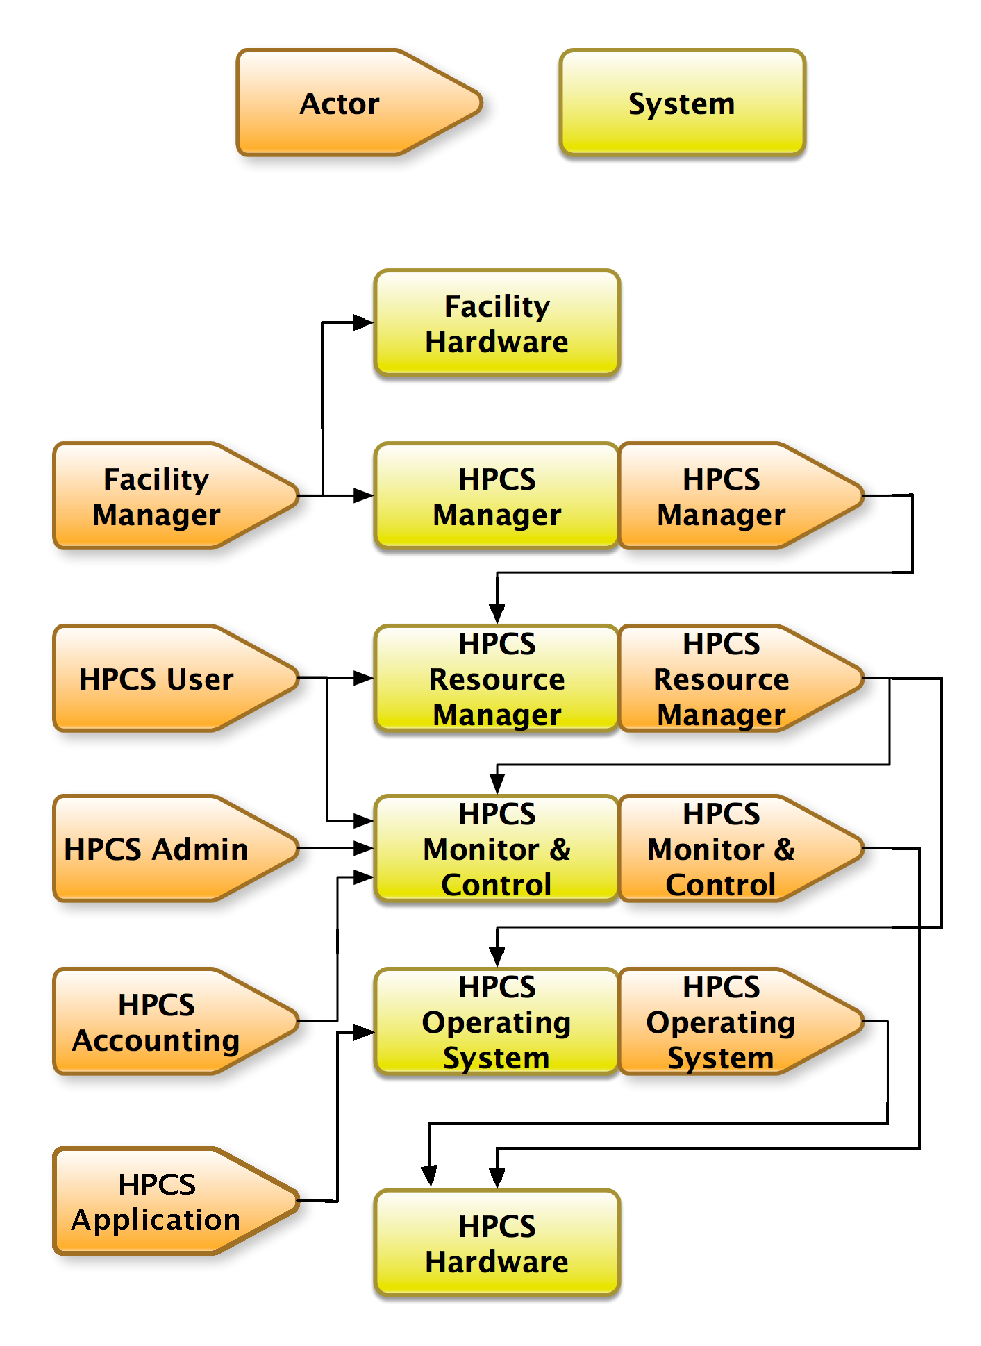
\includegraphics[height=0.6\textheight,width=.69\linewidth]{FIGURES/TopLevelDiagram}
    \end{center}
\caption{Top Level Conceptual Diagram representing the culmination of all Use Case Diagrams covered.}
\label{fig:UCDTopLevel}
\end{figure}

The specific actor/system pairs used for the power API are shown in Figure \ref{fig:UCDTopLevel}.
The external actors are shown on the left portion of the diagram. 
Systems are shown as rectangles. 
The four systems conjoined with the actor symbol also serve as actors for some use cases. 
The ten sections within Chapter \ref{chap:Interfaces} provide function specifications for the ten actor/system pairs (Role/System pairs in the specification).
The two missing interfaces are Facility Manager to Facility Hardware and Facility Manager to HPCS manager.
These were included in the use case model to identify the boundaries of the specification and recognize important points of information input. 

\section{Security Model}\label{sec:SecModel}
The specification assumes traditional hardware (e.g. protection rings) and operating system support for access control.
Implementations should only need traditional restrictions based on authenticated individual identity and/or the groups to which the individual belongs.
A super user is likely needed as well.
Depending on the implementation, the context structure (Section \ref{sec:ContextTypeDefinitions}) may be sufficiently protected to allow for secure storage of access information. Future releases of the specification will address security and policy considerations in more detail.


	\chapter{Theory of Operation}\label{chap:Theory}
	
%=============================================================================%
%=============================================================================%
%=============================================================================%
%=============================================================================%
%=============================================================================%
%=============================================================================%
%=============================================================================%
\section{Overview}
This section discusses many of the foundational concepts leveraged throughout the Power API specification.
It should be noted that many terms commonly used when discussing object oriented languages are used in this section and the document as a whole.
The use of these terms in no way implies that the Power API specification must be implemented using an object oriented language.
%The authors of this specification in fact, recommend the contrary.
We have attempted to achieve two goals, listed in order of priority: 1) programmer portability, where the programmer is the user of the API, and 2) the latitude of the implementor who will often become the user of the API benefitting from our first priority. 

%=============================================================================%
%=============================================================================%
%=============================================================================%
%=============================================================================%
%=============================================================================%
%=============================================================================%
%=============================================================================%
\section{Power API Initialization}\label{sec:PowerAPIInit}


Using any of the Power API interfaces requires initialization. 
Initializaton returns a context.
In the specification, the context is defined as an opaque pointer.
This approach was taken to allow the maximum amount of flexibility to the implementor.
The context returned will contain (act as the entry point to) the system description that is exposed to the user, all policy and privilege information, basically everything the user of the API requires to perform the functionality specified by the API.
The system description is not required to be changed or updated during the life of a specific context.
Initialization is accomplished by calling \funcref{CntxtInit}.
Resources created, like groups, by the user during the life of the context should be cleaned up (destroyed) by the user when no longer needed. 
The implementation is required to clean up all context resources when the user calls \funcref{CntxtDestroy}.

%=============================================================================%
%=============================================================================%
%=============================================================================%
%=============================================================================%
%=============================================================================%
%=============================================================================%
%=============================================================================%
\section{Roles}\label{sec:Roles}

The Power API specification leverages the concept of Roles. 
Roles represent the different types of users that exist which include:
\begin{itemize}[noitemsep,nolistsep] %
\item{\textbf{Application}  The application or application library executing on the compute resource. May also include run-time components running in user space.}
\item{\textbf{Monitor and Control}  Cluster management or Reliability Availability and Serviceability (RAS) systems, for example.}
\item{\textbf{Operating System} Linux or specialized Light Weight Kernels which are found on HPC platforms and potentially portions of run-time systems. }
\item{\textbf{User} The user of the HPC platform. }
\item{\textbf{Resource Manager} This can include work load managers, schedulers, allocators and even portions of run-time systems. }
\item{\textbf{Administrator} The system administrator or HPC platform manager. }
\item{\textbf{HPCS Manager} The individual or individuals responsible for managing policy for the HPC platform, for example. }
\item{\textbf{Accounting} Individual or software that produces reports of metrics for the HPC platform. }
\end{itemize}
These brief definitions are not meant to be exhaustive.
Roles are analogous with the \textit{Actors} discussed in section \ref{sec:UseCase}.
In some cases roles become the system that other roles interact with.
For example, we specify an interface between the Application role (HPCS Application in figure \ref{fig:UCDTopLevel}) and the Operating System (HPCS Operating System in figure \ref{fig:UCDTopLevel}).
The Operating System is the system (in UML terminology) that the Application role is interacting with. 
Notice in figure \ref{fig:UCDTopLevel} that the specification also includes an interface between the Operating System role and the Hardware (HPCS Hardware in figure \ref{fig:UCDTopLevel}).
These and other interfaces are described in chapter \ref{chap:Interfaces}.
The user of the API is required to specify what role they will assume when interacting with the system upon initialization of the API.

%The implementation is required to associate an integer precedence with each role, zero (0) being the highest precedence.
%Roles may have the same precedence number which indicates the roles have equal precedence.
%Other factors, such as user name and permissions can be used to make precedence determinations at finer granularity.
%This feature is provided as a mechanism for the implementation to determine which operation has priority especially in cases where operations conflict.

%For example, the Administrator role (assigned precedence 0) sets a power cap for node 0 at 200W. 
%The Resource Manager role (assigned precedence 1) would like to manage the power cap for an application which uses a number of nodes including node 0.
%The Application role (assigned precedence 2) would like to fine tune the power cap of one of the nodes it is executing on (node 0). 
%The implementation can use the precedence numbers in a variety of ways given the assumptions above.
%In this scenario, the Administrator role is allowed to set the power cap for node 0 at 200W.
%If the Resource Manager requests a power cap of 210W for node 0 the operation would be denied given a role with higher precedence requested a lower power cap.
%If the Resource Manager requests a power cap of 180W for node 0, the operation is allowed.
%Likewise the Application role is permitted to request a lower power cap for node 0 but not a higher power cap.
%First note, the specification does not proscribe these rules, it only provides the precedence mechanism as a way to implement them.
%Also note, this example could be accomplished by simply determining precedence based on which role is requesting the operation.
%The precedence concept is provided in cases where, for example, the implementation requires two roles to have equal precedence.
%If we add to the above scenario the Operating System role (precedence 0), the Operating System has the ability to request that the power cap for node 0 be raised to 210W.
%Once more the specification is not proscribing this rule, only illustrating the need for an additional mechanism that can be used by the implementation to enforce similar scenarios.
%
%\laros{Add a reference here for the call that can be used to get the implementation assigned precedence numbers for each role.}

Roles are also provided as a mechanism for the implementation to express priority or precedence in circumstances where, for example, conflicting operations are requested. 
%More detail on this topic is provided in section \ref{sec:Initialization} (Initialization).


%=============================================================================%
%=============================================================================%
%=============================================================================%
%=============================================================================%
%=============================================================================%
%=============================================================================%
%=============================================================================%
\section{System Description}\label{sec:PowerAPIBaseSysDesc}

\begin{figure}
	\begin{center}
		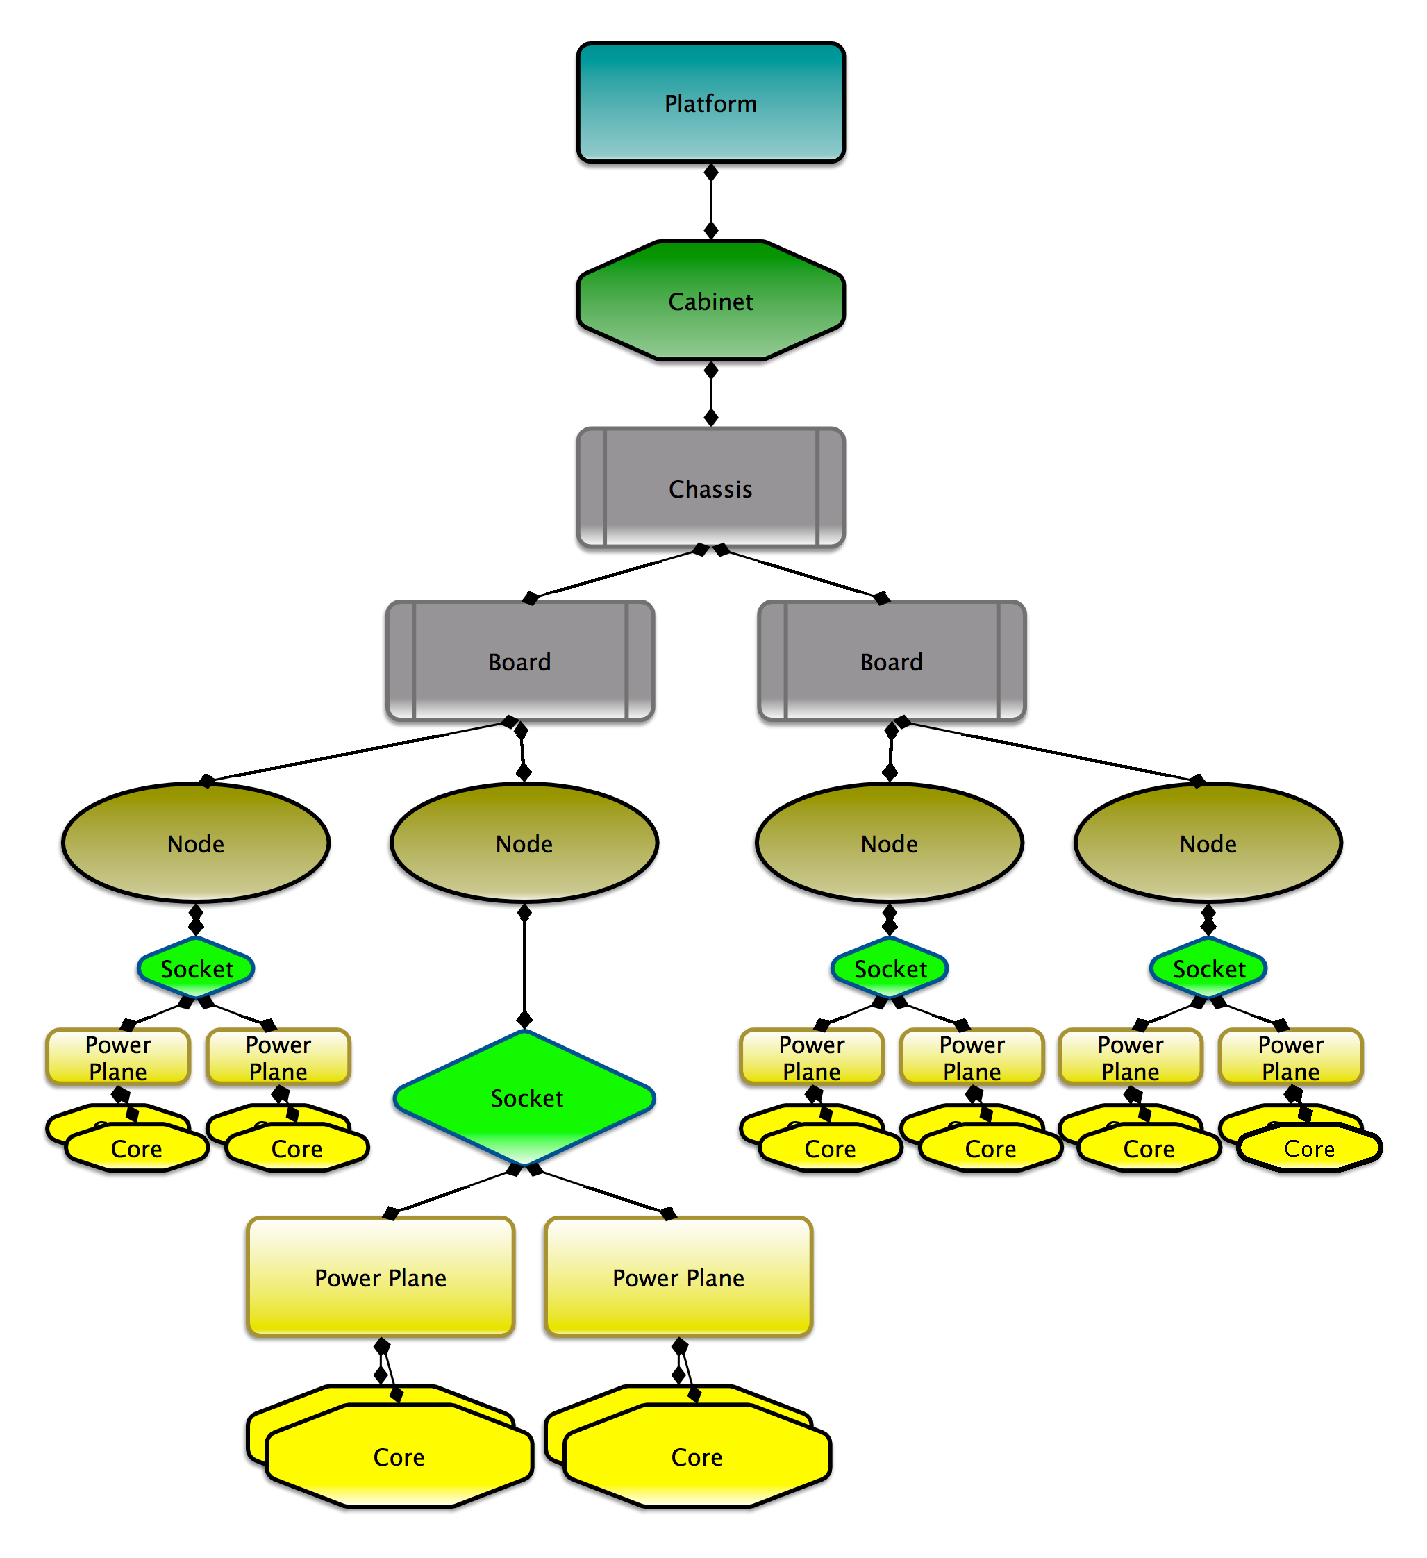
\includegraphics[width=0.80\linewidth,height=.60\paperheight]{FIGURES/PowerAPIMachineHierarchy5dot1}
	\end{center}
	\caption{Hierarchical Depiction of System Objects}
	\label{fig:BaseSystemMap}
\end{figure}

The system description is the \textit{view} of the system exposed to the user upon initialization via the context that is returned.
Figure \ref{fig:BaseSystemMap} depicts an example of a system description showing a hierarchical arrangement of objects.
All object types listed in the specification must be defined by any implementation, but do not have to be used in the system description.
The implementation chooses which objects will be employed in the system description and how they will be arranged.
An object can only have a single parent but may have multiple children.
Currently, a system description may only describe a single platform and have a single object of type \texttt{Platform} which represents the top of the hierarchy. 
Later revisions of the specification may include the ability to combine multiple platforms in the system description. 
This might be useful, for example, in representing an entire datacenter. 
While figure \ref{fig:BaseSystemMap} depicts a homogeneous system description, homogeneity is \textit{not} a requirement. 
In practice a system description can be heterogeneous and unbalanced.

To summarize the requirements:
\begin{itemize}[noitemsep,nolistsep] %
	\item{
	The \texttt{Platform} object type must be defined by the implementation and must appear at the top of the system description.
	}
	\item{
	All object types in this specification must be defined in any implementation. The use of the object types, with the exception of the \texttt{Platform} object type, is optional.
	}
	\item{
	Objects can only have one parent but may have many children. Currently the \texttt{Platform} object has no parent since it appears at the top of the system description. This will likely change in future versions of the specification.
	}
        \item{
        If an implementation chooses to add objects not defined in the specification they should only be exposed to the user in a vendor specific context to avoid unpredictable or non-portable behaviour (see \funcref{CntxtInit}).
        }
\end{itemize}

%Figure \ref{fig:BaseSystemMap} depicts a hierarchical arrangement of all of the  platform objects that must be included (defined) in any implementation of the API.
%In addition to the requirement that these object types must be defined in any implementation, they also must be organized in the order shown in figure \ref{fig:BaseSystemMap}.
%For example, an implementation must always position objects of type \textit{Cabinet} under the top level \textit{Platform} object.
%Likewise, objects of type \textit{Board} must appear below an object of type \textit{Cabinet}.
%There can only be a single object of type \textit{Platform}, and that object must be the top of the hierarchy.

The following is a list of the object types currently included in the specification along with a short description of each.
\begin{itemize}[noitemsep,nolistsep] %
	\item{
Platform - Currently, the one and only Platform object is the top level object of the system description exposed to the user of the API. 
The Platform object is intended to conceptually represent the entire Platform.
For example, if the Platform object has a power or energy measurement or control capability exposed through the Platform objects attributes the scope of these attributes should be platform wide.
}
	\item{
Cabinet - Objects of type Cabinet are intended to represent the cabinets or racks that act as enclosures (or logical groupings) for the platform equipment. 
Beyond the utility of convenient groups of lower level objects (equipment) cabinets may have power or energy relevant capabilities which can be exposed through attributes associated with each Cabinet object. 
}
	\item{
Chassis - Objects of type Chassis are intended to be used for finer grained organization of objects within the higher level Cabinet object. Chassis, like cabinets may have power or energy relevant capabilities that can be exposed to the user.
}
	\item{
Board - Board objects offer another method of organization for underlying objects (equipment). 
Boards may also have power and or energy relevant capabilities which can be exposed through associated attributes. 
For example, a board could contain the power supply and the point of instrumentation for collecting power or energy samples for a node or multiple nodes.
}
	\item{
Node - The Node type is probably one of the most universally important object types. 
Measuring and controlling the power and or energy characteristics of a node or multiple nodes (grouped into multiple Boards, Chassis or Cabinets) is important for a many reasons and provides a wide range of flexibility of configuration to the implementor. 
For example, on HPC platforms a single application typically executes on many nodes. 
Understanding the energy use of an application run can be obtained by collecting the energy use (via the appropriate Node attribute) for each node participating in that application execution. 
Node objects will likely have many attributes exposing many power and energy relevant capabilities.
}
	\item{
Socket - The Socket object is intended to represent the one or more processor sockets, or other component types that can be thought of as sockets, that make up a Node. 
For example, a single Node object may be a dual socket (dual CPU) node.
The implementor may choose to enclose other component types (a NIC for example) within a Socket object, or add other object types as they see fit to represent the architecture they are describing.
They can also decide to omit the use of this, or any other object type (currently other than Platform) in the system description.
}
	\item{
Power Plane - The Power Plane object is used to organize lower level objects (any types of objects) within a power domain or single point of measurement and or control.
For example, a pair of cores may share a power plane within a socket. 
This configuration is depicted in figure \ref{fig:BaseSystemMap}. 
This organization allows a pair of cores to be controlled from a single power control point in the hierarchy for convenience. 
This object type allows these power and energy relevant relationships to be expressed anywhere in the system description.
}
	\item{
Core - Core objects are intended to represent the individual processor cores within multi-core CPUs (or possibly GPUs). 
Modern architectures have an increasing number of cores per CPU (or GPU). 
In the near future it is likely that an abstraction between Socket and core would become useful as the number of cores increase. 
Physical and logical groupings of cores already exist in current architectures.
}
	\item{Memory - The Memory object type is included to represent the growing range of memory types that exist on HPC platforms. 
Individual cores, for example, have Memory in the form of cache which the implementor may choose to organize differently from the main memory of the Node or a tertiary level of memory such as NVRAM.
}	
	\item{
NIC - The NIC object is intended to represent the Network Interface Controller.
As with many other object types, the organization of a NIC in relation to Boards, Nodes or even Cores is architecture dependent.
The NIC object type is included in hopes that there are power and energy relevant capabilities included in future NICs.
}	
        \item{
HT - The HT (Hardware Thread) object represents an OS-visible CPU.  
While from a physical perspective frequency and voltage changes occur at the physical core level, it is usually the case that these must be configured by software at the OS-visible CPU level.  
Typically the lowest-common denominator among all OS-visible CPUs is used to configure the physical core.
}

\end{itemize}

Additional object types may be defined by the implementor and placed anywhere in the hierarchy as long as the previously stated rules are not violated.
Ultimately, the  object types defined in this specification, and those added by the implementor, will be used to produce a system description describing the system presented to the user via the context returned upon initialization.
Objects are used as interfaces to underlying functionality.
The specification does not assume state is retained for objects.
Additionally, the specification makes no guarantees with regards to race conditions between processes or threads.

%=============================================================================%
%=============================================================================%
%=============================================================================%
%=============================================================================%
%=============================================================================%
%=============================================================================%
%=============================================================================%
\section{Attributes}\label{sec:TheoryAttributes}
Attributes are an important part of the Power API.
A large amount of basic functionality is exposed through the use of attributes.
The term attribute is used somewhat conceptually since some attributes are implicit while others are explicitly defined as part of a required specification data structure (page \pageref{type:AttrName}).
Attributes are used for a number of reasons such as to navigate through the system description, to access information or a measurement (sensor information for example) and for control (setting a P-state for example).
Global attributes are attributes that are present for every object defined; whether required by the specification or added by the implementor. 

The following is the list of global attributes:
\begin{itemize}[noitemsep,nolistsep] %
\item{name} - Unique identifying name of the object (see \funcref{ObjGetName}).
\item{entry point} - The position in the hierarchy after initialization (see \funcref{CntxtGetEntryPoint}).
\item{type} - The type of the object (see \funcref{ObjGetType}).
\item{parent} - The parent of an object is the object that is above it in the hierarchy (see \funcref{ObjGetParent}).  The only exception is the currently single platform object whose parent is a pointer to NULL. 
\item{children} -  Object or objects directly below an object in the hierarchy (see \funcref{ObjGetChildren}).
\end{itemize}

Note, in the list above all the attributes are implicit. 
Explicit attributes are defined in the \typeref{AttrName} type definition.
The majority of the attributes defined in the specification, and likely those added by an implementator, are, and will be, explicit.
The implicit attributes defined above are primarily used for navigation and are accessed through attribute specific functions which are described in Section \ref{sec:Navigation}.

Explicit attributes are either accessed through the generic attribute interface (Section \ref{sec:Attributes}) or attribute specific functions found in either the section describing the specific interface in which they are used or in Chapter \ref{chap:Common}, \textit{Core (Common) Interface Functions}.

The attribute interface is intended to keep the specification from growing every time additional functionality is either specified or added by an implementor. 
As long as the new functionality fits within the defined attribute interfaces no additional API functions are required to be specified.

%=============================================================================%
%=============================================================================%
%=============================================================================%
%=============================================================================%
%=============================================================================%
%=============================================================================%
%=============================================================================%
\section{Metadata}\label{sec:TheoryMetadata}
Each object and object attribute pair can have additional descriptive metadata associated with it.
This information is often useful for getting a better understanding of the meaning of objects and attributes and how to interpret the values read from attributes.
Examples include a human readable name and description strings, the list of values supported by an attribute, and measurement accuracy and precision.
The metadata interface (see section \ref{sec:METADATA}) returns information relevant to either a specific object or a specific attribute of a specific object.
A given attribute name may have different metadata for different objects, even if the objects are of the same type (e.g., the voltage attribute of two node objects may have different metadata accuracy values).


\section{Thread Safety}\label{sec:ThreadSafety}
Implementations of the Power API are not required to provide thread safety to multiple threads of the same process.  
If necessary, users of the Power API must use locking or some other mechanism to ensure that only one thread per process calls into the Power API at a time.  
This requirement only applies to threads of the same process that may issue conflicting operations.  
Different processes may make simultaneous Power API calls without any coordination.  
If thread concurrency within a process is required, the \funcref{CntxtInit} function can be called multiple times to initialize multiple Power API contexts.  
Multiple threads of the same process may then simultaneously call into the Power API, so long as each thread operates on a different Power API context.  
For example, a process with four threads may create four Power API contexts and associate one context with each thread.  
The threads may then make Power API calls without any additional coordination, so long as each thread operates only on its assigned context and the objects exposed by its assigned context. 
Threads should not operate on objects exposed by another thread's context without employing locking or some other coordination mechanism.



	\chapter{Type Definitions}\label{chap:TypeDefinitions}
	%==============================================================================%
%==============================================================================%
%==============================================================================%
%==============================================================================%
%==============================================================================%

\section{Opaque Types}\label{sec:OpaqueTypes}

The following type definitions are specified to be opaque pointers from the point of view of Power API users.
Power API implementations will typically map these pointers to internal implementation-specific state.
The reason for using opaque pointers is to hide non-portable implementation details from users and give implementors of the API maximum flexibility.

\begin{typedefs}
	\typedef{void*}{Cntxt}
	\typedef{void*}{Grp}
	\typedef{void*}{Obj}
	\typedef{void*}{Status}
	\typedef{void*}{Stat}
\end{typedefs}

%==============================================================================%
%==============================================================================%
%==============================================================================%
%==============================================================================% 
%==============================================================================%

\section{Globally Relevant Definitions}\label{sec:GlobalTypes}

The following definitions are specified on a global basis.
The \MAJORVERSIONrefx and \defrefx{MINORVERSION} definitions are compile time constants that indicate the Power API version supported by the implementation.
The \defrefx{MAXSTRINGLEN} definition is a compile time constant that defines the maximum length of strings that can be returned from Power API calls, with the actual value being a vendor specific length.

\begin{typedefs}
	\pounddefineMAJORVERSION
	\pounddefineMINORVERSION
	\pounddefineMAXSTRINGLEN
\end{typedefs}

%==============================================================================%
%==============================================================================%
%==============================================================================%
%==============================================================================%
%==============================================================================%

\section{Context Relevant Type Definitions}\label{sec:ContextTypeDefinitions}

The \typeref{CntxtType} and \typerefx{Role} types are required to be defined by all implementations of the Power API.
When a new Power API context is created, one value from each of these types is used to determine the kind of context created (see section \ref{sec:Initialization}).
For \typerefx{CntxtType}, the only required value that an implementation must define is \CNTXTDEFAULTrefx.
This indicates that the new context will only contain Power API functionality that is explicitly defined in the specification, with no implementation-specific extentions present.
Implementors may extend \typerefx{CntxtType} with additional values, such as \CNTXTVENDORrefx, to provide contexts with additional functionality.

We anticipate that most implementations of the Power API will define additional \typerefx{CntxtType} values that provide additional functionality, such as vendor, platform, or model specific extentions.
If an implementation extends the specification, the extensions should only be visible to the user when they use a context that was created with an implementation-specific \typerefx{CntxtType} value.
If the implementation-specific extensions are not available to the user, initialization using an implementation-specific \typerefx{CntxtType} value should result in failure.
The user must always be able to initialize a context using \CNTXTDEFAULTref to to get a context containing only the standard specification features.

Differentiation between context types is the mechanism used by the Power API to enable extended vendor, platform or model specific capabilities while, at the same time, allowing portability for applications or tools that only leverage standard specification features. 
For example, a tool that leverages only the object and attribute types defined in the standard specification can initialize a Power API context using \CNTXTDEFAULTrefx and not have to worry about dealing with any implementation-specific functionality.
The context it receives will only provide functionality that is explicitly defined by the Power API specification.

\typeref{Role} is used to specify the role that the user is acting in when they initialize a new context.
Additional roles may not be added by the implementor.
Notice that there is a role defined for every actor in Chapter \ref{chap:Interfaces} - Role/Systems Interfaces.
We intend that the user's role will serve many purposes, such as determining the view of the system that is provided within the context when combined with the system the user is acting on. 
Roles can also be used to help determine the privilege of the user's context for purposes such as resolving the precedence of conflicting operations.


\subsubsection{PWR_CntxtType}\label{type:CntxtType}
\begin{typedefs}
	\typedef{int}{CntxtType}
	\pounddefineCNTXTDEFAULT
	\pounddefineCNTXTVENDOR
\end{typedefs}


%==============================================================================%

\subsubsection{PWR_Role}\label{type:Role}
\begin{center}
\begin{minipage}{.95\linewidth}%
\begin{lstlisting}
typedef enum {
        PWR_ROLE_APP = 0,   /* Application */
        PWR_ROLE_MC,        /* Monitor and Control */
        PWR_ROLE_OS,        /* Operating System */
        PWR_ROLE_USER,      /* User */
        PWR_ROLE_RM,        /* Resource Manager */
        PWR_ROLE_ADMIN,     /* Administrator */
        PWR_ROLE_MGR,       /* HPCS Manager */
        PWR_ROLE_ACC,       /* Accounting */
        PWR_NUM_ROLES,
        /* */
        PWR_ROLE_INVALID       = -1,
        PWR_ROLE_NOT_SPECIFIED = -2
} PWR_Role;
\end{lstlisting}
\end{minipage}
\end{center}

%==============================================================================%
%==============================================================================%
%==============================================================================%
%==============================================================================%
%==============================================================================%


\section{Object Relevant Type Definitions}\label{sec:ObjectTypeDefinitions}

The \typeref{ObjType} type is required to be defined by all implementations of the Power API specification. 
Objects with types defined by \typerefx{ObjType} are used by the implementor to create the system description (see section \ref{sec:PowerAPIBaseSysDesc}) that is exposed to the user upon initialization.
An implementation may extend this type by adding new object enumeration type, which must be added prior to \texttt{PWR_NUM_OBJ_TYPES}.
The added implementation-specific object types will only be used by implementation-specific contexts (see section \ref{sec:ContextTypeDefinitions}).
Contexts that were initialized using the default context, \texttt{PWR_CNTXT_DEFAULT}, will only expose objects types defined in the list below.

%==============================================================================%

\subsubsection{PWR_ObjType}\label{type:ObjType}
\begin{center}
\begin{minipage}{.95\linewidth}%
\begin{lstlisting}
typedef enum {
        PWR_OBJ_PLATFORM = 0,
        PWR_OBJ_CABINET,
        PWR_OBJ_CHASSIS,
        PWR_OBJ_BOARD,
        PWR_OBJ_NODE,
        PWR_OBJ_SOCKET,
        PWR_OBJ_CORE,
        PWR_OBJ_POWER_PLANE,
        PWR_OBJ_MEM,
        PWR_OBJ_NIC,
        PWR_OBJ_HT,
        PWR_NUM_OBJ_TYPES,
        /* */
        PWR_OBJ_INVALID       = -1,
        PWR_OBJ_NOT_SPECIFIED = -2
} PWR_ObjType;
\end{lstlisting}
\end{minipage}
\end{center}



%==============================================================================%
%==============================================================================%
%==============================================================================%
%==============================================================================%
%==============================================================================%

\section{Attribute Relevant Type Definitions}\label{sec:AttributeTypeDefinitions}

The \typeref{AttrName} and \typerefx{AttrDataType} types are required to be implemented. 
Both may be extended by the implementor and exposed using an implementation specified context type (see section \ref{sec:ContextTypeDefinitions}).
If new \typerefx{AttrName} entries are added it is required that the attribute name is specified and commented as shown in the \typerefx{AttrName} structure.
Likewise, new types must be added to the \typerefx{AttrDataType} structure. 
It's important to note that the attribute interface currently supports only numeric types.
Attributes should only be added to this definition if they can be meaningfully supported by the attribute interface (section \ref{sec:Attributes}).
Additional attributes must be added prior to  \texttt{PWR_NUM_ATTR_NAMES}.
The Attributes in \typerefx{AttrName} expose what we consider foundational measurement and control interfaces. 
Additional capabilities are and can be added using additional operations and often interface specific functions.

The \typeref{AttrAccessError} type is used to hold the error returns that are popped from the \texttt{PWR_Status} handle (see section \ref{sec:OpaqueTypes}) using the \funcref{StatusPopError} function.

%==============================================================================%

\subsubsection{PWR_AttrName}\label{type:AttrName}
\begin{center}
\begin{minipage}{.95\linewidth}%
\begin{lstlisting}
typedef enum {
        PWR_ATTR_PSTATE = 0,         /* uint64_t */
        PWR_ATTR_CSTATE,             /* uint64_t */
        PWR_ATTR_CSTATE_LIMIT,       /* uint64_t */
        PWR_ATTR_SSTATE,             /* uint64_t */
        PWR_ATTR_CURRENT,            /* double, amps */
        PWR_ATTR_VOLTAGE,            /* double, volts */
        PWR_ATTR_POWER,              /* double, watts */
        PWR_ATTR_POWER_LIMIT_MIN,    /* double, watts */
        PWR_ATTR_POWER_LIMIT_MAX,    /* double, watts */
        PWR_ATTR_FREQ,               /* double, Hz */
        PWR_ATTR_FREQ_LIMIT_MIN,     /* double, Hz */
        PWR_ATTR_FREQ_LIMIT_MAX,     /* double, Hz */
        PWR_ATTR_ENERGY,             /* double, joules */
        PWR_ATTR_TEMP,               /* double, degrees Celsius */
        PWR_ATTR_OS_ID,              /* uint64_t */
        PWR_ATTR_THROTTLED_TIME,     /* uint64_t */
        PWR_ATTR_THROTTLED_COUNT,    /* uint64_t */
        PWR_ATTR_GOV,                /* uint64_t */
        PWR_NUM_ATTR_NAMES,
        /* */
        PWR_ATTR_INVALID       = -1,
        PWR_ATTR_NOT_SPECIFIED = -2
} PWR_AttrName;
\end{lstlisting}
\end{minipage}
\end{center}

%==============================================================================%

\subsubsection{PWR_AttrDataType}\label{type:AttrDataType}
\begin{center}
\begin{minipage}{.95\linewidth}%
\begin{lstlisting}
typedef enum {
        PWR_ATTR_DATA_DOUBLE = 0,
        PWR_ATTR_DATA_UINT64,
        PWR_NUM_ATTR_DATA_TYPES,
        /* */
        PWR_ATTR_DATA_INVALID       = -1,
        PWR_ATTR_DATA_NOT_SPECIFIED = -2
} PWR_AttrDataType;
\end{lstlisting}
\end{minipage}
\end{center}

%==============================================================================%

\subsubsection{PWR_AttrAccessError}\label{type:AttrAccessError}
\begin{center}
\begin{minipage}{.95\linewidth}%
\begin{lstlisting}
typedef struct {
        PWR_Obj      obj;    /* The object associated with the error */
        PWR_AttrName attr;   /* The attribute associated with the error */
        int          index;  /* The index in the output array where the error occurred */
        int          error;  /* The error code, see Error Return Definitions section */
} PWR_AttrAccessError;
\end{lstlisting}
\end{minipage}
\end{center}

%==============================================================================%

\subsubsection{PWR_AttrGov}\label{type:AttrGov}
\begin{center}
\begin{minipage}{.95\linewidth}%
\begin{lstlisting}
typedef enum {
        PWR_GOV_LINUX_ONDEMAND,
        PWR_GOV_LINUX_PERFORMANCE,
        PWR_GOV_LINUX_CONSERVATIVE,
        PWR_GOV_LINUX_POWERSAVE,
        PWR_GOV_LINUX_USERSPACE
} PWR_AttrGov;
\end{lstlisting}
\end{minipage}
\end{center}
%==============================================================================%
%==============================================================================%
%==============================================================================%
%==============================================================================%
%==============================================================================%


\section{Metadata Relevant Type Definitions}\label{sec:MetadataTypeDefinitions}

The \texttt{PWR_MetaName} type is required to be implemented. 
The type may be extended by the implementor and the additional capabilities may be exposed using an implementation specified context type (see section \ref{sec:ContextTypeDefinitions}).
If new \texttt{PWR_MetaName} items are added, it is required that the metadata name be specified and commented as shown in the \texttt{PWR_MetaName} definition. 
Additional metadata items must be added prior to \texttt{PWR_NUM_META_NAMES}.


%==============================================================================%

\subsubsection{PWR_MetaName}\label{type:MetaName}
\begin{center}
\begin{minipage}{.95\linewidth}%
\begin{lstlisting}
typedef enum {
        PWR_MD_NUM = 0,           /* uint64_t */
        PWR_MD_MIN,               /* either uint64_t or double, depending on attribute type */
        PWR_MD_MAX,               /* either uint64_t or double, depending on attribute type */
        PWR_MD_PRECISION,         /* uint64_t */
        PWR_MD_ACCURACY,          /* double */
        PWR_MD_UPDATE_RATE,       /* double */
        PWR_MD_SAMPLE_RATE,       /* double */
        PWR_MD_TIME_WINDOW,       /* PWR_Time */
        PWR_MD_TS_LATENCY,        /* PWR_Time */
        PWR_MD_TS_ACCURACY,       /* PWR_Time */
        PWR_MD_MAX_LEN,           /* uint64_t, max strlen of any returned metadata string. */
        PWR_MD_NAME_LEN,          /* uint64_t, max strlen of PWR_MD_NAME */
        PWR_MD_NAME,              /* char *, C-style NULL-terminated ASCII string */
        PWR_MD_DESC_LEN,          /* uint64_t, max strlen of PWR_MD_DESC */
        PWR_MD_DESC,              /* char *, C-style NULL-terminated ASCII string */
        PWR_MD_VALUE_LEN,         /* uint64_t, max strlen returned by PWR_MetaValueAtIndex */
        PWR_MD_VENDOR_INFO_LEN,   /* uint64_t, max strlen of PWR_MD_VENDOR_INFO */
        PWR_MD_VENDOR_INFO,       /* char *, C-style NULL-terminated ASCII string */
        PWR_MD_MEASURE_METHOD,    /* uint64_t, 0/1 depending on real/model mesurement */
        PWR_NUM_META_NAMES,
        /* */
        PWR_MD_INVALID       = -1,
        PWR_MD_NOT_SPECIFIED = -2
} PWR_MetaName;
\end{lstlisting}
\end{minipage}
\end{center}


%==============================================================================%
%==============================================================================%
%==============================================================================%
%==============================================================================%
%==============================================================================%

\section{Error Return Definitions}\label{sec:ErrorReturnDefinitions}

The following required definitions are the available status returns for the functions described in this specification. 
It is anticipated that this list will grow. 
The implementor is also free to add status returns to express conditions not currently covered in the specification and expose them using an implementation specified context type (see section \ref{sec:ContextTypeDefinitions}).
The range -127 through 128 are reserved for use by the Power API specification.
Positive numbers greater than zero are to be used for warnings.


\begin{center}
\begin{minipage}{.95\linewidth}%
\begin{lstlisting}
#define PWR_RET_WARN_TRUNC 5
#define PWR_RET_WARN_NO_GRP_BY_NAME 4
#define PWR_RET_WARN_NO_OBJ_BY_NAME 3
#define PWR_RET_WARN_NO_CHILDREN 2
#define PWR_RET_WARN_NO_PARENT 1
#define PWR_RET_SUCCESS 0
#define PWR_RET_FAILURE -1
#define PWR_RET_NOT_IMPLEMENTED -2
#define PWR_RET_EMPTY -3
#define PWR_RET_INVALID -4
#define PWR_RET_LENGTH -5
#define PWR_RET_NO_ATTRIB -6
#define PWR_RET_NO_META -7
#define PWR_RET_READ_ONLY -8
#define PWR_RET_BAD_VALUE -9
#define PWR_RET_BAD_INDEX -10
#define PWR_RET_OP_NOT_ATTEMPTED -11
#define PWR_RET_NO_PERM -12
#define PWR_RET_OUT_OF_RANGE -13
#define PWR_RET_NO_OBJ_AT_INDEX -14
\end{lstlisting}
\end{minipage}
\end{center}

%==============================================================================%
%==============================================================================%
%==============================================================================%
%==============================================================================%
%==============================================================================%

\section{Time Related Definitions}\label{sec:TimeRelatedDefinitions}

\texttt{PWR_Time} is defined as a 64-bit value used to hold timestamps in nanoseconds for a wide range of functionality. 
For those timestamps that are to be used in relation to an epoch, midnight January 1st, 1970 will be considered the beginning of the epoch.
This will provide for hundreds of years to be expressed from the epoch point, which is sufficient for the purposes of the Power API.
\texttt{PWR_Time} is also used for other structures designed to record time values (\texttt{PWR_TimePeriod}, page \pageref{type:TimePeriod} for example). 
\texttt{PWR_TIME_UNINIT} is used as an indicator that the time value has not been initialized. 
This is intended to allow the implementation to make decisions on how a function is being used based on whether a time value has been specified or not (for example, the Statistics functions in section \ref{sec:StatisticsFunctions}).
\texttt{PWR_TIME_UNKNOWN} is an output, which indicates that the time of an event was not recorded. For example, a maximum value for an attribute could be known for a given time period, but the instant at which the maximum occurred is unknown.
The \texttt{PWR_TimePeriod} type allows for three timestamps, start, stop and instant. 
Instant is available to indicate when a statistically significant event occurred within the window delineated by start and stop.
For example, if the user requests the \texttt{PWR_ATTR_STAT_MAX} statistic for \texttt{PWR_ATTR_POWER}, the start and stop times will indicate the window of time over which the maximum value was calculated. 
The instant would indicate the instant in time the maximum value occurred.
Defining \texttt{PWR_Time}, \texttt{PWR_TIME_UNINIT}, \texttt{PWR_TIME_UNKNOWN}, and \texttt{PWR_TimePeriod} as specified is required.



\begin{center}
\begin{minipage}{.95\linewidth}%
\begin{lstlisting}
typedef uint64_t PWR_Time;
#define PWR_TIME_UNINIT 0
#define PWR_TIME_UNKNOWN 0 
\end{lstlisting}
\end{minipage}
\end{center}

%==============================================================================%
\subsubsection{PWR_TimePeriod}\label{type:TimePeriod}

\begin{center}
\begin{minipage}{.95\linewidth}%
\begin{lstlisting}
typedef struct {
        PWR_Time    start;
        PWR_Time    stop;
        PWR_Time    instant;
} PWR_TimePeriod;
\end{lstlisting}
\end{minipage}
\end{center}
%==============================================================================%
%==============================================================================%
%==============================================================================%
%==============================================================================%

\section{Statistics Relevant Type Definitions}\label{sec:StatisticTypeDefinitions}
The \texttt{PWR_AttrStat} type includes the list of currently defined statistics potentially available to the user of an implementation.
Potentially, because this feature requires either direct device or software support.
Statistics are generated on a per-attribute basis (see \texttt{PWR_AttrName} on page \pageref{type:AttrName}). 
The statistics type definitions are required to be implemented and are used with the statistics functions (see section \ref{sec:StatisticsFunctions}).

%==============================================================================%

\subsubsection{PWR_AttrStat}\label{type:AttrStat}

\begin{center}
\begin{minipage}{.95\linewidth}%
\begin{lstlisting}
typedef enum {
        PWR_ATTR_STAT_MIN = 0,
        PWR_ATTR_STAT_MAX,
        PWR_ATTR_STAT_AVG,
        PWR_ATTR_STAT_STDEV,
        PWR_ATTR_STAT_CV,
        PWR_ATTR_STAT_SUM,
        PWR_NUM_ATTR_STATS,
        /* */
        PWR_ATTR_STAT_INVALID       = -1,
        PWR_ATTR_STAT_NOT_SPECIFIED = -2
} PWR_AttrStat;
\end{lstlisting}
\end{minipage}
\end{center}

%==============================================================================%


%We probably don't need this anymore as we can use the stat's type for this
%but I'm leaving this in until version 1.1 is released in case we change our
%minds by finding a relevant use case for having this in the spec.
%--REG
%\subsubsection{PWR_StatReduction}\label{type:StatReduction}
%\begin{center}
%\begin{minipage}{.95\linewidth}%
%\begin{lstlisting}
%typedef enum {
%    PWR_ATTR_STAT_REDC_SUM,
%    PWR_ATTR_STAT_REDC_MIN,
%    PWR_ATTR_STAT_REDC_MAX,
%    PWR_ATTR_STAT_REDC_AVG
%} PWR_StatReduction;
%\end{lstlisting}
%\end{minipage}
%\end{center}

\subsubsection{PWR_ID}\label{type:ID}
\begin{center}
\begin{minipage}{.95\linewidth}%
\begin{lstlisting}
typedef enum {
        PWR_ID_USER = 0,
        PWR_ID_JOB,
        PWR_ID_RUN,
        PWR_NUM_IDS,
        /* */
        PWR_ID_INVALID       = -1,
        PWR_ID_NOT_SPECIFIED = -2
} PWR_ID;
\end{lstlisting}
\end{minipage}
\end{center}
%==============================================================================%
%==============================================================================%
%==============================================================================%
%==============================================================================%
%==============================================================================%

\section{OS Hardware Interface Type Definitions}\label{sec:OSHWTypeDefinitions}
The following definitions are used in the Operating system to Hardware interface described in section \ref{sec:OSHW}.
Each definition will be described below along with its specification. All of the definitions in this section are required, even if the corresponding OS/HW functions are not implemented. 


%==============================================================================%

\subsubsection{PWR_OperState}\label{type:OperState}

The \texttt{PWR_OperState} type is used to describe the state being requested by OS to Hardware interface functions that require power/performance state information such as P-State and C-State information. 
Both \texttt{c_state_num} and \texttt{p_state_num} must be provided.

\begin{center}
\begin{minipage}{.95\linewidth}%
\begin{lstlisting}
typedef struct {
        uint64_t c_state_num;
        uint64_t p_state_num;
} PWR_OperState;
\end{lstlisting}
\end{minipage}
\end{center}



%==============================================================================%
%==============================================================================%
%==============================================================================%
%==============================================================================%
%==============================================================================%

\section{Application OS Interface Type Definitions}\label{sec:AppOSTypeDefinitions}
The following definitions are primarily used in the Application to Operating system interface described in section \ref{sec:AppOS}.
Each definition will be described below along with its specification. All of the definitions in this section are required, even if the corresponding App/OS functions are not implemented.

%==============================================================================%
\subsubsection{PWR_RegionHint}\label{type:RegionHint}

The  \texttt{PWR_RegionHint} type is an abstraction intended to allow the application to communicate power and performance significant information to the operating system. It is used in conjunction with \texttt{PWR_RegionIntensity} to describe the type and extent of the behavior described for a given execution region. 
This information can then be used to \textit{tune} components, with the intent being a more power/performance efficient use of the components results. 
For example, if an application is going into a serial region, the performance of the application may benefit from the core running the serial portion of the code at a higher frequency, thereby completing that serial portion faster. 
Since the application is in a serial portion, the implementation may determine that the remaining cores may be put into a more power efficient state (a sleep state for example), thus possibly resulting in both a performance increase and a decrease in the amount of power/energy the application uses.
Regions may be specified as \texttt{PWR_REGION_DEFAULT} to indicate that the application is no longer providing a hint as to the region characteristics of currently executing code.

\begin{center}
\begin{minipage}{.95\linewidth}%
\begin{lstlisting}

typedef enum {
        PWR_REGION_DEFAULT = 0,
        PWR_REGION_SERIAL,
        PWR_REGION_PARALLEL,
        PWR_REGION_COMPUTE,
        PWR_REGION_COMMUNICATE,
        PWR_REGION_IO,
        PWR_REGION_MEM_BOUND,
        PWR_REGION_GLOBAL_LOOP,
        PWR_NUM_REGION_HINTS,
        /* */
        PWR_REGION_INVALID       = -1,
        PWR_REGION_NOT_SPECIFIED = -2
} PWR_RegionHint;

\end{lstlisting}
\end{minipage}
\end{center}

%==============================================================================%

\subsubsection{PWR_RegionIntensity}\label{type:RegionIntensity}

The \texttt{PWR_RegionIntensity} type is an abstraction of a given level of intensity for a \texttt{PWR_RegionHint}.
It provides five levels of intensity as well as \texttt{PWR_Region_INT_NONE}, which can be used in the case where
the intensity is not known, is not applicable, or in cases where the operating system or runtime may be better
equipped to determine the intensity of a given code region.

\begin{center}
\begin{minipage}{.95\linewidth}%
\begin{lstlisting}
typedef enum {
        PWR_REGION_INT_HIGHEST = 0,
        PWR_REGION_INT_HIGH,
        PWR_REGION_INT_MEDIUM,
        PWR_REGION_INT_LOW,
        PWR_REGION_INT_LOWEST,
        PWR_REGION_INT_NONE,
        PWR_NUM_REGION_INTENSITIES,
        /* */
        PWR_REGION_INT_INVALID       = -1,
        PWR_REGION_INT_NOT_SPECIFIED = -2
} PWR_RegionIntensity;
\end{lstlisting}
\end{minipage}
\end{center}

%==============================================================================%

\subsubsection{PWR_SleepState}\label{type:SleepState}

The \texttt{PWR_SleepState} type is a high level abstraction of the different sleep
state levels that may be provided on a given system. The sleep levels are translated into
the appropriate hardware level constructs by lower layers of the PowerAPI. 

\begin{center}
\begin{minipage}{.95\linewidth}%
\begin{lstlisting}
typedef enum {
        PWR_SLEEP_NO = 0,
        PWR_SLEEP_SHALLOW,
        PWR_SLEEP_MEDIUM,
        PWR_SLEEP_DEEP,
        PWR_SLEEP_DEEPEST,
        PWR_NUM_SLEEP_STATES,
        /* */
        PWR_SLEEP_INVALID       = -1,
        PWR_SLEEP_NOT_SPECIFIED = -2
} PWR_SleepState; 
\end{lstlisting}
\end{minipage}
\end{center}

%==============================================================================%

\subsubsection{PWR_PerfState}\label{type:PerfState}

The \texttt{PWR_PerfState} type is an abstraction meant to describe the different
possible performance states in which hardware may be placed.

\begin{center}
\begin{minipage}{.95\linewidth}%
\begin{lstlisting}
typedef enum {
        PWR_PERF_FASTEST = 0,
        PWR_PERF_FAST,
        PWR_PERF_MEDIUM,
        PWR_PERF_SLOW,
        PWR_PERF_SLOWEST,
        PWR_NUM_PERF_STATES,
        /* */
        PWR_PERF_INVALID       = -1,
        PWR_PERF_NOT_SPECIFIED = -2
} PWR_PerfState;
\end{lstlisting}
\end{minipage}
\end{center}




	\chapter{Core (Common) Interface Functions}\label{chap:Common}
	% These have been superceded by the \newenvironment{prototype} macros.  Remove after conversion.
\newcommand{\ArgHdr}{   \begin{center}
			\begin{tabular}{ | p{5cm} | p{2.1cm} | p{7.5cm} |}
			\hline 
			\textbf{Argument(s)} & \textbf{Input } & \textbf{Description} \\  
			 		     & \textbf{and/or} & \\ 
					     & \textbf{Output} & \\ 
			\hline 
}
\newcommand{\ArgLn}[3]{\texttt{#1} & #2 & #3 \\ \hline}
\newcommand{\ArgFtr}{ 	\end{tabular}
			\end{center}
}



Core, or so called Common, interface functions are functions that can be used, at least in par, by most of the interfaces described in the Power API specification. 
Core functions include the following areas:
\begin{itemize}[noitemsep,nolistsep] 
\item{\textbf{Initialization}, required to use any of the functionality described in this specification, }
\item{\textbf{Navigation}  functions allow the user to traverse the system description and discover information about the underlying platform, }
\item{\textbf{Group} functions, primarily a convenience abstraction,}
\item{\textbf{Attribute} functions expose measurement and control functionality, }
\item{\textbf{Metadata} functions allow the user to access additional information about objects and attributes (often device or instrumentation specific information), }
\item{\textbf{Statistics} functions are used to generate statistical information based on fundamental attribute information (measurements),}
\end{itemize}
and other functionality that is common across a number of interfaces.

%=============================================================================%
%=============================================================================%
%=============================================================================%
%=============================================================================%
%=============================================================================%
%=============================================================================%

\section{Initialization}\label{sec:Initialization}

Initialization using \texttt{PWR_CntxtInit} is required to use any of the functionality documented in this specification.
The user supplies the type of the context requested and their role. 
Currently, the specification's only required context type is \texttt{PWR_CNTXT_DEFAULT}.
The context type is intended to be one way in which the implementor can distinguish their implementation from the standard specification and other implementations (see section \ref{sec:ContextTypeDefinitions}).
The user must also supply their role (see page \pageref{type:Role} for the \texttt{PWR_Role} definition).
One purpose of specifying the role is to convey what type of user they intend to be, and therefore, how they would like to interact with or how the underlying implementation manages the privileges granted to the user/role combination.
A system administrator (\texttt{PWR_ROLE_ADMIN}) will desire and require different capabilities, privileges and level of abstraction than the application user (\texttt{PWR_ROLE_APP}), for example.

The user also has the opportunity to specify a name that will be associated with the context. 
This \textit{feature} is anticipated to be useful in supporting advanced functionality.
Initialization returns a context to the user.
The context contains the user's view of the system, dependent on what type of context was requested, the user's role and implementation specifics.
The system description that the user is exposed to must conform to the rules outlined in the specification (see sections \ref{sec:PowerAPIInit} and \ref{sec:PowerAPIBaseSysDesc}).
The context should be destroyed (cleaned up) by using the \texttt{PWR_CntxtDestroy} function when no longer needed.

%=============================================================================%
%int PWR_CntxtInit( PWR_CntxtType type, PWR_Role role, const char* name, PWR_Cntxt* context);
\begin{prototype}{CntxtInit}
	\longdescription{ The \PWR{CntxtInit} function is required to be called before using any other Power API function.  The context returned is passed to other Power API functions either explicitly as an argument or implicitly through an argument associated with the context.
	}
	\pnote{See page \pageref{type:CntxtType} for a discussion of contexts and roles.}
	\returntype{int}
	\parameter{\PWR{CntxtType} type}{\pInput} 	{The requested context type.}
	\parameter{\PWR{Role} role}	{\pInput} 	{The role of the user.}
	\parameter{const char* name}  	{\pInput} 	{User specified string name to be associated with the context.}
	\parameter{\PWR{Cntxt}* context}{\pOutput}	{The user's context.}
	\returnval{\PWR{RET_SUCCESS}}			{Upon SUCCESS, context is set to a valid user context.}
	\returnval{\PWR{RET_FAILURE}}			{Upon FAILURE.}
\end{prototype}

%=============================================================================%
%int    PWR_CntxtDestroy( PWR_Cntxt context );
\begin{prototype}{CntxtDestroy}
	\longdescription{The \PWR{CntxtDestroy} function is used to destroy (clean up) the context obtained with \PWR{CntxtInit}. The implementation is required to clean up, unlink, destroy (as appropriate) all context resources as a result of this call.}
	\returntype{int}
	\parameter{PWR_Cntxt context}{\pInput}{The context obtained using \PWR{CntxtInit} the user wishes to destroy.}
	\returnval{\PWR{RET_SUCCESS}}	{Upon SUCCESS.}
	\returnval{\PWR{RET_FAILURE}}	{Upon FAILURE.}
\end{prototype}

%=============================================================================%
%=============================================================================%
%=============================================================================%
%=============================================================================%
%=============================================================================%
%=============================================================================%
%=============================================================================%


\section{Hierarchy Navigation Functions}\label{sec:Navigation}

Hierarchy navigation (also called discovery) is accomplished using attributes (EntryPoint, Type, Parent and Children) that are implicit to every object in the system description whether defined in the specification or added by the implementor.
Navigation is accomplished using these attributes, through the associated function calls, within the context made available to the user upon initialization.
After initialization the first call will generally be \texttt{PWR_CntxtGetEntryPoint} to determine the user's entry point in the system hierarchy provided within the user's context. 
Depending on the user, the interface and the role, the context could contain a view of the entire system description or a subset of the system description.
Navigating through the hierarchy is accomplished with \texttt{PWR_ObjGetParent} to navigate up and \texttt{PWR_ObjGetChildren} to navigate down.
To understand what kind of object was returned with either of these calls the user can utilize \texttt{PWR_ObjGetType} call.
The name of the object can be discovered using the \texttt{PWR_ObjGetName} function and if the user has a name, the associated object can be discovered using the \texttt{PWR_CntxtGetObjByName} function. 

The Power API does not provide an explicit ``Free Object'' interface.
Specifically, objects returned by Power API interfaces do not need to be later freed or released explicitly.
This design choice was made in order to keep usage of the Power API as simple as possible, with the potential cost of an increased burden on the Power API implementor to limit implementation-internal memory usage.


%=============================================================================%
%int    PWR_CntxtGetEntryPoint( PWR_Cntxt context, PWR_Obj* entry_point );
\begin{prototype}{CntxtGetEntryPoint}
	\longdescription{The \texttt{PWR_CntxtGetEntryPoint} call is typically used immediately following initialization.  Whenever \texttt{PWR_CntxtGetEntryPoint} is called the implementation defined entry point (location) in the system description is returned.  \texttt{PWR_CntxtGetEntryPoint} can always be called to reposition or reorient the user to the initial entry location.}
	\returntype{int}
	\parameter{PWR_Cntxt context}   {\pInput} 	{The user's context.}
	\parameter{PWR_Obj* entry_point}{\pOutput}	{The user's entry point into the system description (the same for the life of the context).}
	\returnval{PWR_RET_SUCCESS} 			{ Upon SUCCESS, entry_point set to system description entry point (object).}	
	\returnval{PWR_RET_FAILURE} 			{ Upon FAILURE.}
\end{prototype}

%=============================================================================%
%int    PWR_ObjGetType( PWR_Obj object, PWR_ObjType* type );
\begin{prototype}{ObjGetType}
	\longdescription{ The \texttt{PWR_ObjGetType} function returns the type of the object specified.  See page \pageref{type:ObjType} for valid object types.}
	\returntype{int}
	\parameter{PWR_Obj object}	{\pInput}	{The object that the user wishes to determine the type of.}
	\parameter{PWR_ObjType* type}	{\pOutput}	{The type of the specified object.}
	\returnval{PWR_RET_SUCCESS} 	{ Upon SUCCESS, type is set to the type of the specified object.}
	\returnval{PWR_RET_FAILURE} 	{ Upon FAILURE, type is set to PWR_OBJ_INVALID.}
\end{prototype}
%=============================================================================%
%int    PWR_ObjGetName( PWR_Obj object, char* dest, size_t len );
\begin{prototype}{ObjGetName}
	\longdescription{The \texttt{PWR_ObjGetName} function copies the name of the specified object into the user provided buffer.  See page \pageref{func:CntxtGetObjByName} to get the object based on the unique name using \texttt{PWR_CntxtGetObjByName}.}
	\returntype{int}
	\parameter{PWR_Obj object}	{\pInput}	{The object that the user wishes to determine the name of.}
	\parameter{char* dest}    	{\pInput}	{The address of the user provided buffer.}
	\parameter{size_t len}    	{\pInput}	{The length of the user provided buffer.}
	\returnval{PWR_RET_SUCCESS} 	{Upon SUCCESS, the buffer will contain the name of the object, the string will include a terminating null byte.}	
	\returnval{PWR_RET_WARN_TRUNC} 	{Call succeeded, but the length of object name was longer than the provided buffer and the name was truncated.}
	\returnval{PWR_RET_FAILURE} 	{Upon FAILURE.}
\end{prototype}
%==============================================================================%
%int PWR_ObjGetParent( PWR_Obj object, PWR_Obj* parent );
\begin{prototype}{ObjGetParent}
	\longdescription{The \texttt{PWR_ObjGetParent} function is used to find the object immediately above the specified object in the system description available to the user through the current context.  Note, currently, there are some cases where an object has no parent, namely the platform object.}
	\returntype{int}
	\parameter{PWR_Obj object} {\pInput} 		{The object that the user wishes to determine the parent of.}
	\parameter{PWR_Obj* parent}{\pOutput}		{The parent object of the specified input object.}
	\returnval{PWR_RET_SUCCESS}        		{Upon SUCCESS, parent set to parent of specified object.}
	\returnval{PWR_RET_WARN_NO_PARENT} 		{Call succeeded but specified object does not have a parent.}
	\returnval{PWR_RET_FAILURE}        		{Upon FAILURE.}
\end{prototype}

%==============================================================================%
%int     PWR_ObjGetChildren( PWR_Obj object, PWR_Grp* group );
\begin{prototype}{ObjGetChildren}
	\longdescription{The \texttt{PWR_ObjGetChildren} function returns the child or children of the specified object.  The caller is expected to check the return code of \texttt{PWR_ObjGetChildren} to determine if the object has children or not.  If the specified object has one or more children, indicated by a return code of \texttt{PWR_RET_SUCCESS}, a new group (\texttt{PWR_Grp}) is returned that contains the object's children.  The user is responsible for destroying this group when it is no longer needed (see \texttt{PWR_GrpDestroy} on page \pageref{func:GrpDestroy}).  If the specified object has no children, indicated by a return code of \texttt{PWR_RET_WARN_NO_CHILDREN}, no group is returned and the input (\texttt{PWR_Grp}) is not modified.}
	\returntype{int}
	\parameter{PWR_Obj objec}	{\pInput}	{The object that the user wishes to determine the children of.}
	\parameter{PWR_Grp* group}	{\pOutput}	{On input, this should be set to point to an uninitialized \texttt{PWR_Grp} (i.e., the caller should not call \texttt{PWR_GrpCreate} ahead of time).  If \texttt{PWR_RET_SUCCESS} is returned, *group will be set to a newly created group containing the \texttt{object}'s children.  If \texttt{PWR_RET_WARN_NO_CHILDREN} is returned, the input \texttt{PWR_Grp} is not modified.}
	\returnval{PWR_RET_SUCCESS}          		{Upon SUCCESS, group is set to a newly created group containing the child or children of specified object.}
	\returnval{PWR_RET_WARN_NO_CHILDREN} 		{Call succeeded but specified object does not have any children. The input \texttt{PWR_Grp} is not modified.}
	\returnval{PWR_RET_FAILURE}          		{Upon FAILURE.}
\end{prototype}

%=============================================================================%
%int    PWR_CntxtGetObjByName( PWR_Cntxt context, const char* name, PWR_Obj* object);
\begin{prototype}{CntxtGetObjByName}
	\longdescription{The \texttt{PWR_CntxtGetObjByName} function returns the object given the context and unique object name.  See page \pageref{func:ObjGetName} to get the name of a specified object using \texttt{PWR_ObjGetName}.}
	\returntype{int}
	\parameter{PWR_Cntxt context}	{\pInput}{The context containing the object that the user wishes to retrieve given its unique name. Note, the object may be present in the system but not available to the user through the current context.}
	\parameter{const char * name}	{\pInput}{The unique name of the object that the user wishes to retrieve.}
	\parameter{PWR_Obj* object}	{\pOutput}{The object that corresponds to the name specified by the user.}
	\returnval{PWR_RET_SUCCESS}             	{Upon SUCCESS, object is set to object corresponding to name specified by user.}
	\returnval{PWR_RET_WARN_NO_OBJ_BY_NAME} 	{If no object exists corresponding to name provided.}
	\returnval{PWR_RET_FAILURE}             	{Upon FAILURE.}
\end{prototype}

%==============================================================================%
%=============================================================================%
%=============================================================================%
%=============================================================================%
%=============================================================================%
%=============================================================================%
%=============================================================================%
\section{Group Functions}\label{sec:Group}

Group functions are provided as a convenience in situations, for example, where an operation, or operations are required to be executed on multiple objects. 
Rather than executing the same operation multiple times, once for each object, some operations provide a group variant to streamline this type of functionality.
Groups can be dynamically created (\texttt{PWR_GrpCreate}) when needed and can exist for short periods of time and destroyed with \texttt{PWR_GrpDestroy}, or exist for the duration of the users context.
Groups may not contain multiple instances of the same object, i.e. duplicate objects are not allowed.
When a new group is the product of a function (\texttt{PWR_GrpUnion, PWR_GrpIntersection, PWR_GrpDifference}) and the result of the function operation is the empty set (no objects) an empty group (group with no objects)  should be the result and the function should return \texttt{PWR_RET_SUCCESS}. 
It is the responsibility of the user to clean up all groups produced as a result of group functions using \texttt{PWR_GrpDestroy}.
Groups can only contain objects from a single \texttt{PWR_cntxt}.
Group operations that involve multiple groups must be performed with groups from the same context.

%int PWR_GrpCreate( PWR_Cntxt context, PWR_Grp* group );
\begin{prototype}{GrpCreate}
	\longdescription{The \texttt{PWR_GrpCreate} function is used to create a new group which will be associated with and unique to the users context.}
	\returntype{int}
	\parameter{PWR_Cntxt context}	{\pInput} {The user's context that the group, when created, will be associated with.}
	\parameter{PWR_Grp* group}   	{\pOutput}{The new (empty) group.}
	\returnval{PWR_RET_SUCCESS} 	{Upon SUCCESS, group is set to new (empty) group.}
	\returnval{PWR_RET_FAILURE} 	{Upon FAILURE.}
\end{prototype}

%=============================================================================%
%int PWR_GrpDestroy( PWR_Grp group );
\begin{prototype}{GrpDestroy}
	\longdescription{The \texttt{PWR_GrpDestroy} function is used to destroy (clean up) a group created by a user.}
	\returntype{int}
	\parameter{PWR_Grp group}{\pInput}{The group that the user is acting on.}
	\returnval{PWR_RET_SUCCESS} 	{Upon SUCCESS.}
	\returnval{PWR_RET_FAILURE} 	{Upon FAILURE.}
\end{prototype}

%=============================================================================%
%int PWR_GrpAddObj( PWR_Grp group, PWR_Obj object );
\begin{prototype}{GrpAddObj}
	\longdescription{The \texttt{PWR_GrpAddObj} function is used to add a specified object to a specified group.  Duplicate objects are not allowed in groups.  Adding an object that would be a duplicate of one already in the group will result in no insertion and returns \texttt{PWR_RET_SUCCESS}.}
	\returntype{int}
	\parameter{PWR_Grp group} 	{\pInputOutput}	{The group that the user is acting on.}
	\parameter{PWR_Obj object}	{\pInput}       {The object to be added to the specified group.}
	\returnval{PWR_RET_SUCCESS} 	{Upon SUCCESS.}
	\returnval{PWR_RET_FAILURE} 	{Upon FAILURE.}
\end{prototype}

%=============================================================================%
%int PWR_GrpRemoveObj( PWR_Grp group, PWR_Obj object );
\begin{prototype}{GrpRemoveObj}
	\longdescription{The \texttt{PWR_GrpRemoveObj} function is used to remove a specified object from a specified group.  Attempting to remove an object that is not a member of a group will result in \texttt{PWR_RET_SUCCESS}.}
	\returntype{int}
	\parameter{PWR_Grp group} 	{\pInputOutput}	{The group that the user is acting on.}
	\parameter{PWR_Obj object}	{\pInput}       {The object to be removed from the specified group.}
	\returnval{PWR_RET_SUCCESS}  	{Upon SUCCESS.}
	\returnval{PWR_RET_FAILURE}  	{Upon FAILURE.}
\end{prototype}
%=============================================================================%
%int PWR_GrpGetNumObjs( PWR_Grp group );
\begin{prototype}{GrpGetNumObjs}
	\longdescription{The \texttt{PWR_GrpGetNumObjs} function is used to get the number of objects contained in the specified group.} \returntype{int} \parameter{PWR_Grp group}{\pInput}{The group that the user is acting on.}
	\returnval{int} 		{Upon SUCCESS, the number of objects contained in the specified group.}
	\returnval{PWR_RET_FAILURE} 	{Upon FAILURE.}
\end{prototype}

%=============================================================================%
%int PWR_GrpGetObjByIndx( PWR_Grp group, int index, PWR_Obj* object);
\begin{prototype}{GrpGetObjByIndx}
	\longdescription{The \texttt{PWR_GrpGetObjByIndx} is used to get the object from the specified group at the specified index.}
	\returntype{int}
	\parameter{PWR_Grp group}  {\pInput} {The group that the user is acting on.}
	\parameter{int  index}     {\pInput} {The index within the specified group of the desired object.}
	\parameter{PWR_Obj* object}{\pOutput}{The object at the specified index in the specified group.}
	\returnval{PWR_RET_SUCCESS} 		{Upon SUCCESS, object is set to object at specified index.}
	\returnval{PWR_RET_NO_OBJ_AT_INDEX} 	{No object at specified index in specified group.}
	\returnval{PWR_RET_FAILURE} 		{Upon FAILURE.}
\end{prototype}
%=============================================================================%
%int PWR_GrpDuplicate( PWR_Grp group1, PWR_Grp* group2 );
\begin{prototype}{GrpDuplicate}
	\longdescription{The \texttt{PWR_GrpDuplicate} function is used to duplicate an existing group.  The duplicate group is a new separate group from the original group specified.  Actions on the duplicate group do not affect the original group and vice versa.}
	\returntype{int}
	\parameter{PWR_Grp group1}	{\pInput}{The original group (group1).}
	\parameter{PWR_Grp* group2}	{\pOutput}{Duplicate (group2) of the original group (group1) specified by user even if the original group contains no objects.}

	\returnval{PWR_RET_SUCCESS} 	{Upon SUCCESS, duplicate group of original group created.}
	\returnval{PWR_RET_FAILURE} 	{Upon FAILURE.}
\end{prototype}

%=============================================================================%
%int PWR_GrpUnion( PWR_Grp group1, PWR_Grp group2, PWR_Grp* group3);
\begin{prototype}{GrpUnion}
	\longdescription{The \texttt{PWR_GrpUnion} function is used to create a group that is the union ($\cup$) of two specified groups.  The union group created is a new separate group from the original groups specified.  Actions on the union group do not affect the original groups and vice versa.}
	\returntype{int}
	\parameter{PWR_Grp group1}	{\pInput}{The first of the two groups used in the union, ($\cup$) operation.}
	\parameter{PWR_Grp group2}	{\pInput}{The second of the two groups used in the union, ($\cup$) operation.}
	\parameter{PWR_Grp* group3}	{\pOutput}{he output group (group3) is the union, ($\cup$) operation, of the first (group1) and second (group2) groups specified. If the result of the union operation is the empty set group3 is an empty group (valid group with no objects).}
	\returnval{PWR_RET_SUCCESS} 	{Upon SUCCESS, group3 contains the union of group1 and group2.}
	\returnval{PWR_RET_FAILURE} 	{Upon FAILURE.}
\end{prototype}

%=============================================================================%
%int PWR_GrpIntersection( PWR_Grp group1, PWR_Grp group2, PWR_Grp* group3);
\begin{prototype}{GrpIntersection}
	\longdescription{The \texttt{PWR_GrpIntersection} function is used to create a group that is the Intersection ($\cap$) of two specified groups.  The intersection group is a new separate group from the original groups specified.  Actions on the intersection group do not affect the original groups and vice versa.}
	\returntype{int}
	\parameter{PWR_Grp group1}	{\pInput}{The first of the two groups used in the Intersection ($\cap$)  operation.}
	\parameter{PWR_Grp group2}	{\pInput}{The second of the two groups used in the intersection ($\cap$) operation.}
	\parameter{PWR_Grp* group3}	{\pOutput}{The output group (group3) is the intersection, ($\cap$) operation, of the first (group1) and second (group2) groups specified. If the result of the intersection operation is the empty set group3 is an empty group (valid group with no objects).}
	\returnval{PWR_RET_SUCCESS} 	{Upon SUCCESS, group3 contains the intersection of group1 and group2.}
	\returnval{PWR_RET_FAILURE} 	{Upon FAILURE.}
\end{prototype}

%=============================================================================%
%int PWR_GrpDifference( PWR_Grp group1, PWR_Grp group2, PWR_Grp* group3 );
\begin{prototype}{GrpDifference}
	\longdescription{The \texttt{PWR_GrpDifference} function is used to create a group that is the Difference ($\setminus$) of two specified groups.  The difference group is a new separate group from the original groups specified.  Actions on the difference group do not affect the original groups and vice versa.  In the event that the output \texttt{PWR_Grp} contains no objects see~\ref{sec:Group} for the definition of the output, \texttt{PWR_Grp}.}
	\returntype{int}
	\parameter{PWR_Grp group1}	{\pInput}{The first of the two groups used in the difference ($\setminus$)  operation.}
	\parameter{PWR_Grp group2}	{\pInput}{The second of the two groups used in the difference ($\setminus$) operation.}
	\parameter{PWR_Grp* group3}	{\pOutput}{The output group (group3) is the difference, ($\setminus$) operation, of the first (group1) and second (group2) groups specified. If the result of the difference operation is the empty set group3 is an empty group (valid group with no objects).}
	\returnval{PWR_RET_SUCCESS} 	{Upon SUCCESS,  group3 contains the difference of group1 and group2.}
	\returnval{PWR_RET_FAILURE} 	{Upon FAILURE.}
\end{prototype}

%=============================================================================%

\subsubsection{Function Prototype for PWR_GrpSymDifference()}\label{func:GrpSymDifference}
%int PWR_GrpSymDifference( PWR_Grp group1, PWR_Grp group2, PWR_Grp* group3 );
\begin{prototype}{GrpSymDifference}
	\longdescription{The \texttt{PWR_GrpSymDifference} function is used to create a group that is the Symmetric Difference ($\triangle$) of two specified groups.  The symmetric difference group is a new separate group from the original groups specified.  Actions on the symmetric difference group do not affect the original groups and vice versa.  In the event that the output \texttt{PWR_Grp} contains no objects see~\ref{sec:Group} for the definition of the output, \texttt{PWR_Grp}.}
	\returntype{int}
	\parameter{PWR_Grp group1}{Input}{The first of the two groups used in the symmetric difference ($\triangle$)  operation.}
	\parameter{PWR_Grp group2}{Input}{The second of the two groups used in the symmetric difference ($\triangle$) operation.}
	\parameter{PWR_Grp* group3}{Output}{The output group (group3) is the symmetric difference, ($\triangle$) operation, of the first (group1) and second (group2) groups specified. If the result of the symmetric difference operation is the empty set group3 is an empty group (valid group with no objects).}
	\returnval{PWR_RET_SUCCESS} 	{Upon SUCCESS,  group3 contains the symmetric difference of group1 and group2.}
	\returnval{PWR_RET_FAILURE} 	{Upon FAILURE.}
\end{prototype}

%=============================================================================%
% int   PWR_CntxtGetGrpByName( PWR_Cntxt context, const char* name, PWR_Grp* group);
\begin{prototype}{CntxtGetGrpByName}
	\longdescription{The \texttt{PWR_CntxtGetGrpByName} function returns a group in a given context via a unique group name.  This function is included to allow the user to make use of groups that are provided with the initial context by the implementation.  The list of valid group names should be provided by the vendor in their documentation.  Due to the defined group names being vendor specific, use of this function should be considered non-portable.  The group returned by this call must be functionally identical to a group created via \texttt{PWR_GrpCreate()}.  Like a group created with \texttt{PWR_GrpCreate()} groups returned by \texttt{PWR_CntxtGetGrpByName()} must be destroyed with the \texttt{PWR_GrpDestroy()} call.}
	\returntype{int}
	\parameter{PWR_Cntxt context}	{\pInput}	{The context containing the group that the user wishes to retrieve given its unique name.}
	\parameter{const char* name}	{\pInput}	{The unique name of the group that the user wishes to retrieve.}
	\parameter{PWR_grp* group}	{\pOutput}	{The implementation provided group corresponding to the specified name.}
	\returnval{PWR_RET_SUCCESS}        		{Upon SUCCESS, group corresponding to the specified name.}
	\returnval{PWR_RET_WARN_NO_GRP_BY_NAME} 	{If no implementation supplied group exists corresponding to name provided.}
	\returnval{PWR_RET_FAILURE}             	{Upon FAILURE.}
\end{prototype}

%=============================================================================%
%=============================================================================%
%=============================================================================%
%=============================================================================%
%=============================================================================%
%=============================================================================%
%=============================================================================%

\section{Attribute Functions}\label{sec:Attributes}

The Attribute functions make up the foundation of the Power API specification, providing measurement (get) and control (set) interfaces for a wide range of power and energy related functionality.
Get and set interfaces are provided for single attribute/single object, multiple attribute/single object, single attribute/multiple objects (group) and multiple attributes/multiple objects (group).
In each case the user specifies the attribute or attributes to get or set.
The valid attribute names are defined in the \texttt{PWR_AttrName} structure (see page \pageref{type:AttrName}).
A complete list of all the valid attributes and their meanings can be found in table \ref{table:MasterAttributeTable}, section \ref{sec:BLOA}.
The timestamp is a critical part of the get (measurement) interface for power and energy related information.
It is very important that the timestamp returned (\texttt{PWR_Time}) be an accurate representation of when the value returned was measured to the best possible temporal accuracy, not when the function was called.
It is required by the specification that the value returned is the value that was measured as close as possible to when the get function was called.
The quality of the measurement and timestamp are device and implementation dependent.
Information about each attribute can be obtained through the metadata interface, described in section \ref{sec:METADATA}.

%
%==============================================================================%
%int PWR_ObjAttrGetValue( PWR_Obj object, PWR_AttrName attr, void* value, PWR_Time* ts );
\begin{prototype}{ObjAttrGetValue}
	\longdescription{The \texttt{PWR_ObjAttrGetValue} function is provided to get the value of a single specified attribute (\texttt{PWR_AttrName attr}) from a single specified object (\texttt{PWR_Obj object}).  The timestamp returned (\texttt{PWR_Time *ts}) should accurately represent when the value was measured.}
	\returntype{int}
	\parameter{PWR_Obj object}	{\pInput}	{The target object.}
	\parameter{PWR_AttrName attr}	{\pInput}	{The target attribute. See section \ref{type:AttrName} for a list of available attributes}
	\parameter{void* value}		{\pOutput}	{Pointer to caller-allocated storage, of 8 bytes, to hold the value read from the attribute.}
	\parameter{PWR_Time* ts}	{\pOutput}	{Pointer to caller-allocated storage to hold the timestamp of when the value was read from the attribute. Pass in \texttt{NULL} if the timestamp is not needed.}
	\returnval{PWR_RET_SUCCESS} 			{Upon SUCCESS.}
	\returnval{PWR_RET_NOT_IMPLEMENTED} 		{The requested attribute is not supported for the target object.}
	\returnval{PWR_RET_FAILURE} 			{Upon FAILURE.}
\end{prototype}
%==============================================================================%
%int PWR_ObjAttrSetValue( PWR_Obj object, PWR_AttrName attr, const void* value );
\begin{prototype}{ObjAttrSetValue}
	\longdescription{The \texttt{PWR_ObjAttrSetValue} function is provided to set the value of a single specified attribute (\texttt{PWR_AttrName attr}) of a single specified object (\texttt{PWR_Obj object}).}
	\returntype{int}
	\parameter{PWR_Obj object}	{\pInput}	{The target object.}
	\parameter{PWR_AttrName attr}	{\pInput}	{The target attribute. See section \ref{type:AttrName} for a list of available attributes.}
	\parameter{const void* value}	{\pInput}	{Pointer to the 8 byte value to write to the attribute.}
	\returnval{PWR_RET_SUCCESS} 			{Upon SUCCESS.}
	\returnval{PWR_RET_NOT_IMPLEMENTED} 		{The requested attribute is not supported for the target object.}
	\returnval{PWR_RET_BAD_VALUE} 			{The value was not appropriate for the target attribute.}
	\returnval{PWR_RET_OUT_OF_RANGE} 		{The value was out of range for the target attribute.}
	\returnval{PWR_RET_FAILURE} 			{Upon FAILURE.}
\end{prototype}
%==============================================================================%
%int PWR_StatusCreate( PWR_Cntxt context, PWR_Status* status );
\begin{prototype}{StatusCreate}
	\longdescription{The \texttt{PWR_StatusCreate} function is provided to create the \texttt{PWR_Status} object that will be used in functions that perform multiple operations and potentially return individual statuses for each operation.  It is up to the implementation to create the appropriate amount of storage for the \texttt{PWR_Status} structure based on the implementation and the number of statuses that will be held.  \texttt{PWR_Status} objects can only be used in the context in which they are created, attempting to use a \texttt{PWR_Status} object in a context other than the one it was created for will result in an error.  For example see \texttt{PWR_ObjAttrGetValues} on page \pageref{func:ObjAttrGetValues}.  Note, \texttt{PWR_Status} is an opaque handle, its backing definition is determined by the implementor (see \ref{sec:OpaqueTypes}).  It is intended that the implementation only allocate space for failed operations.  Errors are read from the \texttt{PWR_Status} by popping them off the structure which requires the structure to only be as large as the number of error returns require.  When status objects are passed into a function, they are automatically cleared, therefore errors should always be checked on a status object before reuse.  \emph{Note to Users: Caution is advised when reusing status objects in multiple threads. Common thread safety practices must be followed to ensure that errors are properly caught. Creating status objects for each thread is advised to avoid potential race conditions.}}
	\returntype{int}
	\parameter{PWR_Cntxt context}	{\pInput}	{The context in which the new status is to be used.}
	\parameter{PWR_Status* status}	{\pOutput}	{The new status structure.}
	\returnval{PWR_RET_SUCCESS} 	{Upon SUCCESS.}
	\returnval{PWR_RET_FAILURE} 	{Upon FAILURE.}
\end{prototype}
%==============================================================================%
%int PWR_StatusDestroy( PWR_Status status );
\begin{prototype}{StatusDestroy}
	\longdescription{The \texttt{PWR_StatusDestroy} function is provided to 	destroy the \texttt{PWR_Status} object created using \texttt{PWR_StatusCreate} (see page \pageref{func:StatusCreate}.  Note, \texttt{PWR_Status} is an opaque handle, its backing definition is determined by the implementor (see \ref{sec:OpaqueTypes}).}
	\returntype{int}
	\parameter{PWR_Status status}	{\pInput}	{The \texttt{PWR_Status} structure the user wishes to destroy.}
	\returnval{PWR_RET_SUCCESS} 	{Upon SUCCESS.}
	\returnval{PWR_RET_FAILURE} 	{Upon FAILURE.}
\end{prototype}
%==============================================================================%
%int PWR_StatusPopError( PWR_Status status, PWR_AttrAccessError* error );
\begin{prototype}{StatusPopError}
	\longdescription{The \texttt{PWR_StatusPopError} function is provided to iterate through the \texttt{PWR_Status} object created using \texttt{PWR_StatusCreate} (see page \pageref{func:StatusCreate}) and populated using any of the function calls that leverage this structure.  Using this method allows the \texttt{PWR_Status} structure to only grow as large as necessary storing only error returns.  Note, \texttt{PWR_Status} is an opaque handle, its backing definition is determined by the implementor (see \ref{sec:OpaqueTypes}). The \texttt{PWR_AttrAccessError} structure that is returned will always have its \texttt{obj}, \texttt{attr}, and \texttt{error} fields set to the object, attribute, and error code associated with the error.  The \texttt{PWR_AttrAccessError} structure's index field will only be set for attribute get functions (e.g., \texttt{PWR_ObjAttrGetValues}), and indicates the index in the output value array where the error occurred.  For attribute get functions, errors are returned by \texttt{PWR_StatusPopError} in ascending order by index.}
	\returntype{int}
	\parameter{PWR_Status status}		{\pInput}	{The \texttt{PWR_Status} structure the user wishes to examine (iterate over).}
	\parameter{PWR_AttrAccessError* error}	{\pOutput}	{Pointer to a  \texttt{PWR_AttrAccessError} structure (see page \pageref{type:AttrAccessError}) to hold the status that is popped from the \texttt{PWR_Status} structure.}
	\returnval{PWR_RET_SUCCESS} {Upon SUCCESS.}
	\returnval{PWR_RET_EMPTY}   {Returned when all errors have been popped.}
	\returnval{PWR_RET_FAILURE} {Upon FAILURE.}
\end{prototype}

%==============================================================================%
%int PWR_StatusClear( PWR_Status status )
\begin{prototype}{StatusClear}
	\longdescription{The \texttt{PWR_StatusClear} function is provided to clear a previously used \texttt{PWR_Status} object created using \texttt{PWR_StatusCreate}, (see page \pageref{func:StatusCreate}) basically allowing reuse of the same structure if multiple calls are executed and examined in sequence.  Note, \texttt{PWR_Status} is an opaque handle, its backing definition is determined by the implementor (see \ref{sec:OpaqueTypes}).}
	\returntype{int}
	\parameter{PWR_Status status}	{\pInput}	{The \texttt{PWR_Status} structure the user wishes to clear (reuse).}
	\returnval{PWR_RET_SUCCESS} 	{Upon SUCCESS.}
	\returnval{PWR_RET_FAILURE} 	{Upon FAILURE.}
\end{prototype}

%==============================================================================%
%int PWR_ObjAttrGetValues( PWR_Obj object, int count, const PWR_AttrName attrs[], void* values, PWR_Time ts[], PWR_Status status );
\begin{prototype}{ObjAttrGetValues}
	\longdescription{The \texttt{PWR_ObjAttrGetValues} function is provided to get the value of multiple specified attributes listed in the \texttt{PWR_AttrName attrs[]} array from a single specified object -- \textbf{get multiple attribute values from a single object}.  The timestamps returned in the \texttt{PWR_Time ts[]} array should accurately represent, and correspond sequentially, with the time each value returned was measured.  If the function fails for one or more attributes, the \texttt{PWR_Status status} structure returned can be examined for additional information regarding the failure using \texttt{PWR_StatusPopError} (see page \pageref{func:StatusPopError}).}
	\returntype{int}
	\parameter{PWR_Obj object}		{\pInput}{The target object.}
	\parameter{int count}			{\pInput}{The number of elements in the \texttt{attrs[]}, \texttt{*values}, and \texttt{ts[]} arrays.}
	\parameter{const PWR_AttrName attrs[]}	{\pInput}{The array of target attributes to read. See section \ref{type:AttrName} for a list of available attributes.}
	\parameter{void* values}		{\pOutput}	{The array of values read, one value for each target attribute. This should point to caller-allocated storage of at least (\texttt{count * 8}) bytes. Upon success, the value read for attribute \texttt{attrs[i]} will be located at address (\texttt{values+(i*8)}).}
	\parameter{PWR_Time ts[]}		{\pOutput}{The array of timestamps, one timestamp for each value read. This should point to caller-allocated storage of at least (\texttt{count*sizeof(PWR_Time)}). Upon success, the timestamp of the value read for \texttt{attrs[i]} will be located at ts[i]. Pass in \texttt{NULL} if timestamps are not needed.}
	\parameter{PWR_Status status}		{\pOutput}{Upon \texttt{PWR_RET_FAILURE}, \texttt{status} contains information about each failure that occurred. Pass in \texttt{NULL} if failure information is not needed.}

	\returnval{PWR_RET_SUCCESS} 		{Upon SUCCESS, all operations succeeded.}
	\returnval{PWR_RET_FAILURE} 		{Upon FAILURE, one or more operations failed. Examine \texttt{PWR_Status* status} to determine the operations that failed. All other operations succeeded.}
\end{prototype}
%==============================================================================%
%int PWR_ObjAttrSetValues( PWR_Obj object, int count, const PWR_AttrName attrs[], const void* values, PWR_Status status );
\begin{prototype}{ObjAttrSetValues}
	\longdescription{The \texttt{PWR_ObjAttrSetValues} function is provided to set the value of multiple specified attributes in the  (\texttt{PWR_AttrName attrs[]}) array of a specified object -- \textbf{set multiple attribute values of a single object}.  If the function fails for one or more attributes, the \texttt{PWR_Status status} structure returned can be examined for additional information regarding the failure using \texttt{PWR_StatusPopError} (see page \pageref{func:StatusPopError}).}
	\returntype{int}

	\parameter{PWR_Obj object}		{\pInput}{The target object.}
	\parameter{int count}			{\pInput}{The number of elements in the \texttt{attrs[]} and \texttt{*values} arrays.}
	\parameter{const PWR_AttrName attrs[]}	{\pInput}{The array of target attributes to write. See section \ref{type:AttrName} for a list of available attributes.}
	\parameter{const void* values}		{\pInput}{The array of values to write, one value for each target attribute. The value to write to attribute \texttt{attrs[i]} is located at address (\texttt{values+(i*8)}).}
	\parameter{PWR_Status status}		{\pOutput}{Upon \texttt{PWR_RET_FAILURE}, \texttt{status} contains information about each failure that occurred. Pass in \texttt{NULL} if failure information is not needed.}
	\returnval{PWR_RET_SUCCESS} 		{Upon SUCCESS, all operations succeeded.}
	\returnval{PWR_RET_FAILURE} 		{Upon FAILURE, one or more operations failed. Examine \texttt{PWR_Status* status} to determine the operations that failed. All other operations succeeded.}
\end{prototype}
%==============================================================================%
%int PWR_ObjAttrIsValid( PWR_Obj object, PWR_AttrName attr );
\begin{prototype}{ObjAttrIsValid}
	\longdescription{The \texttt{PWR_ObjAttrIsValid} function is used to determine if a specified attribute (\texttt{PWR_AttrName attr}) is valid for the specified object.}
	\returntype{int}
	\parameter{PWR_Obj object}	{\pInput}{The object that the user is acting on.}
	\parameter{PWR_AttrName attr}	{\pInput}{The attribute the user wishes to confirm is valid for the specified object.  See the \texttt{PWR_AttrName} type definition in section \ref{type:AttrName}.}
	\returnval{PWR_RET_SUCCESS} {Upon SUCCESS.}
	\returnval{PWR_RET_FAILURE} {Upon FAILURE.}
\end{prototype}

%==============================================================================%
%int PWR_GrpAttrGetValue( PWR_Grp group, PWR_AttrName attr, void* values, PWR_Time ts[], PWR_Status status );
\begin{prototype}{GrpAttrGetValue}
	\longdescription{The \texttt{PWR_GrpAttrGetValue} function is provided to get the value of a single specified attribute (\texttt{PWR_AttrName attr}) from all the objects in a specified group (\texttt{PWR_Grp group}) -- \textbf{get a single attribute value from multiple objects}.  The timestamps returned in the \texttt{PWR_Time ts[]} array should accurately represent, and correspond sequentially, with the time each value returned was measured.  If the function fails for one or more attributes, the \texttt{PWR_Status status} structure returned can be examined for additional information regarding the failure using \texttt{PWR_StatusPopError} (see page \pageref{func:StatusPopError}).  \texttt{PWR_GrpAttrGetValue} will continue to attempt to gather values for the entire group, even if an error occurs for a subset of the members of that group.}
	\returntype{int}
	\parameter{PWR_Grp group}	{\pInput}{The target group.}
	\parameter{PWR_Attrgame attr}	{\pInput}{The target attribute to retrieve (get) from each object in the target group. See section \ref{type:AttrName} for a list of available attributes.}
	\parameter{void* values}	{\pOutput}{The array of attribute values retrieved, one value for each object in the target group. This should point to caller-allocated storage of at least (\texttt{PWR_GrpGetNumObjs() * 8}) bytes. Upon success, the value retrieved for the object at index \texttt{i} within the group will be located at address (\texttt{values+(i*8)}).}
	\parameter{PWR_Time ts[]}	{\pOutput}{The array of timestamps, one timestamp for each value retrieved. This should point to caller-allocated storage of at least (\texttt{PWR_GrpGetNumObjs()*sizeof(PWR_Time)}). Upon success, the timestamp of the value retrieved for the object at index \texttt{i} within the group will be located at ts[i]. Pass in \texttt{NULL} if timestamps are not needed.}
	\parameter{PWR_Status status}	{\pOutput}{Upon \texttt{PWR_RET_FAILURE}, \texttt{status} contains information about each failure that occurred. Pass in \texttt{NULL} if failure information is not needed.}

	\returnval{PWR_RET_SUCCESS} 	{Upon SUCCESS, all operations succeeded.}
	\returnval{PWR_RET_FAILURE} 	{Upon FAILURE, one or more operations failed. Examine \texttt{PWR_Status* status} to determine the operations that failed. All other operations succeeded.}
\end{prototype}
%=============================================================================%
%int PWR_GrpAttrSetValue( PWR_Grp group, PWR_AttrName attr, const void* value, PWR_Status status );
\begin{prototype}{GrpAttrSetValue}
	\longdescription{The \texttt{PWR_GrpAttrSetValue} function is provided to set the value of a single specified attribute (\texttt{PWR_AttrName attr}) of each object in a specified group -- \textbf{set a single attribute value on multiple objects}.  If the function fails for one or more attributes, the \texttt{PWR_Status status} structure returned can be examined for additional information regarding the failure using \texttt{PWR_StatusPopError} (see page \pageref{func:StatusPopError}).  \texttt{PWR_GrpAttrSetValue} will continue to attempt to set values for the entire group, even if an error occurs for a subset of the members of that group.}
	\returntype{int}
	\parameter{PWR_Grp group}	{\pInput}{The target group.}
	\parameter{PWR_AttrName attr}	{\pInput}{The target attribute to set for each object in the target group. See section \ref{type:AttrName} for a list of available attributes.}
	\parameter{const void* value}	{\pInput}{The pointer to a single 8 byte attribute value to set for each object in the target group.}
	\parameter{PWR_Status status}	{\pOutput}{Upon \texttt{PWR_RET_FAILURE}, \texttt{status} contains information about each failure that occurred. Pass in \texttt{NULL} if failure information is not needed.}
	\returnval{PWR_RET_SUCCESS} 	{Upon SUCCESS, all operations succeeded.} 
	\returnval{PWR_RET_FAILURE} 	{Upon FAILURE, one or more operations failed. Examine \texttt{PWR_Status* status} to determine the operations that failed. All other operations succeeded.}
\end{prototype}
%=============================================================================%
%int PWR_GrpAttrGetValues( PWR_Grp group, int count, const PWR_AttrName attrs[], void* values, PWR_Time ts[], PWR_Status status );
\begin{prototype}{GrpAttrGetValues}
	\longdescription{The \texttt{PWR_GrpAttrGetValues} function is provided to get the value of multiple specified attributes listed in the \texttt{PWR_AttrName attrs[]} array from each object in a specified group -- \textbf{get multiple attribute values from multiple objects}.  The timestamps returned in the \texttt{PWR_Time ts[]} array should accurately represent, and correspond sequentially, with the time each value returned was measured.  If the function fails for one or more attributes, the \texttt{PWR_Status status} structure returned can be examined for additional information regarding the failure using \texttt{PWR_StatusPopError} (see page \pageref{func:StatusPopError}).  \texttt{PWR_GrpAttrGetValues} will continue to attempt to gather values for the entire group, even if an error occurs for a subset of the members or attributes requested in the object group.}
	\returntype{int}
	\parameter{PWR_Grp group}		{\pInput}{The target group.}
	\parameter{int count}			{\pInput}{The number of elements in the \texttt{attrs[]} array.}
	\parameter{const PWR_AttrName attrs[]}	{\pInput}{he array specifying the set of target attributes to read for each object in the target group. See section \ref{type:AttrName} for a list of available attributes.}
	\parameter{void* values}		{\pOutput}{The array of attribute values retrieved. This should point to caller-allocated storage of at least (\texttt{PWR_GrpGetNumObjs()*count*8}) bytes.  Upon success, the value read for attribute \texttt{attrs[i]} for the object at index \texttt{j} within the group will be located at address (\texttt{values+(j*count*8)+(i*8)}).}
	\parameter{PWR_Time ts[]}{Output}{The array of timestamps, one timestamp for each value retrieved. This should point to caller-allocated storage of at least (\texttt{PWR_GrpGetNumObjs()*count*sizeof(PWR_Time)}). Upon success, the timestamp of the value retrieved for attribute \texttt{attrs[i]} for the object at index \texttt{j} within the group will be located at ts[(j*count)+i]. Pass in \texttt{NULL} if timestamps are not needed.}
	\parameter{PWR_Status status}		{\pOutput}{Upon \texttt{PWR_RET_FAILURE}, \texttt{status} contains information about each failure that occurred. Pass in \texttt{NULL} if failure information is not needed.}
	\returnval{PWR_RET_SUCCESS} {Upon SUCCESS, all operations succeeded.}
	\returnval{PWR_RET_FAILURE} {Upon FAILURE, one or more operations failed. Examine \texttt{PWR_Status* status} to determine the operations that failed. All other operations succeeded.}
\end{prototype}
%=============================================================================%
%int PWR_GrpAttrSetValues( PWR_Grp group, int count, const PWR_AttrName attrs[], const void* values, PWR_Status status );
\begin{prototype}{GrpAttrSetValues}
	\longdescription{The \texttt{PWR_GrpAttrSetValues} function is provided to set the value of multiple specified attributes listed in the  (\texttt{PWR_AttrName attrs[]}) array of each object in a specified group -- \textbf{set multiple attribute values on multiple objects}.  If the function fails for one or more attributes, the \texttt{PWR_Status status} structure returned can be examined for additional information regarding the failure using \texttt{PWR_StatusPopError} (see page \pageref{func:StatusPopError}).  \texttt{PWR_GrpAttrSetValues} will continue to attempt to set values for the entire group and requested attributes, even if an error occurs for a subset of the members or attributes of that object group.}
	\returntype{int}
	\parameter{PWR_Grp group}		{\pInput}{The target group.}
	\parameter{int count}			{\pInput}{The number of elements in the \texttt{attrs[]} and \texttt{*values} arrays.}
	\parameter{const PWR_AttrName attrs[]}	{\pInput}{The array specifying the set of target attributes to set for each object in the target group. See section \ref{type:AttrName} for a list of available at     tributes.}
	\parameter{const void* values}		{\pInput}{The array of attribute values to set for each object in the group. The value to write to attribute \texttt{attrs[i]} of each object is located at address (\texttt{values+(i*8)}).}
	\parameter{PWR_Status status}		{\pOutput}{Upon \texttt{PWR_RET_FAILURE}, \texttt{status} contains information about each failure that occurred. Pass in \texttt{NULL} if failure information is not needed.}
	\returnval{PWR_RET_SUCCESS} {Upon SUCCESS, all operations succeeded.}
	\returnval{PWR_RET_FAILURE} {Upon FAILURE, one or more operations failed. Examine \texttt{PWR_Status* status} to determine the operations that failed. All other operations succeeded.}
\end{prototype}
%=============================================================================%
%==============================================================================%
%=============================================================================%
%=============================================================================%
%=============================================================================%
%=============================================================================%
%=============================================================================%
%=============================================================================%
\section{Metadata Functions}\label{sec:METADATA}

The metadata functions provide an interface for getting more descriptive
information about an object or attribute, such as estimated measurement
accuracy or the list of valid values for a given attribute.  This
information is often useful for getting a better understanding of the
meaning of objects and attributes and how to interpret the values read
from attributes.  While most metadata is read-only information, some
metadata is potentially configurable, such as the underlying power
sampling rate used to calculate \texttt{PWR_ATTR_ENERGY} values.

Table~\ref{table:MasterMetadataTable} on page~\pageref{type:AttrStat} 
lists the available types of metadata. Not all of the metadata items
listed will be available for every object and attribute pair.  The exact
set is dependent on the capabilities of the underlying hardware and
Power API implementation. If a requested metadata item is not available
a \texttt{PWR_RET_NO_ATTRIB} error is returned at runtime.

The majority
of metadata items will require that both an object instance and
attribute name pair be specified, but a few may be defined for object
instances alone.  For example, the metadata strings \texttt{PWR\_MD\_NAME},
\texttt{PWR\_MD\_DESC}, and \texttt{PWR\_MD\_VENDOR\_INFO} may be
available for individual object instances, with no associated attribute
name specified.  In these cases, the attribute name requested should
be set to \texttt{PWR_ATTR_NOT_SPECIFIED}. One important use case for
these informational strings, especially the \texttt{PWR\_MD\_VENDOR\_INFO}
string, is for a Power API user to capture these strings with each run
to record configuration and provenance information.  For example, a
user may chose to log the \texttt{PWR\_MD\_VENDOR\_INFO} string for
the top-level platform object in the output of each run.

The metadata interface consists of three functions. The
\texttt{PWR_ObjAttrGetMeta} and \texttt{PWR_ObjAttrSetMeta} functions allow
metadata values to be retrieved and set, respectively. The third function,
\texttt{PWR_MetaValueAtIndex}, provides a way to enumerate through an attribute's
list of available values.  This is useful for attributes that have a small, well-defined
set of discrete values (e.g., \texttt{PWR\_ATTR\_PSTATE}). It is expected that where 
a set of discrete values can be described in a logical order that the index ordering
is from smallest (lowest) to largest (highest) value. The remainder of
this section describes the metadata functions in more detail.

%
%==============================================================================%
%int PWR_ObjAttrGetMeta( PWR_Obj obj, PWR_AttrName attr, PWR_MetaName meta, void* value );
\begin{prototype}{ObjAttrGetMeta}
	\longdescription{The \texttt{PWR_ObjAttrGetMeta} function returns the requested metadata item for the specified object or object and attribute name pair.  The caller must allocate enough storage to hold the returned metadata value and pass a pointer to the storage in the \texttt{value} argument.  The required size can be determined by consulting the type column of Table~\ref{table:MasterMetadataTable}.  In the case of string metadata items (i.e., type \texttt{char *}), the required string length can be determined by getting the appropriate length metadata item, which is the original metadata name with the \texttt{_LEN} suffix added.  For example, the required string length for the \texttt{PWR_MD_VENDOR_INFO} string can be determined by retrieving the \texttt{PWR_MD_VENDOR_INFO_LEN} metadata item.}
	\parameter{PWR_Obj obj}		{\pInput}{The target object.}
	\parameter{iPWR_AttrName attr}	{\pInput}{The target attribute. See the \texttt{PWR_AttrName} type definition in Section \ref{type:AttrName} for the list of possible attributes. If object-only metadata is being requested, this argument should be set to \texttt{PWR_ATTR_NOT_SPECIFIED}.}
	\parameter{PWR_MetaName meta}	{\pInput}{The target metadata item to get. See the \texttt{PWR_MetaName} type definition in Section \ref{type:MetaName} for the list of possible metadata items, with detailed descriptions provided in Table~\ref{table:MasterMetadataTable}.}
	\parameter{void* value}		{\pOutput}{Pointer to the caller allocated storage to hold the value of the requested metadata item. See Table~\ref{table:MasterMetadataTable} for type information.}
	\returnval{PWR_RET_SUCCESS} 	{Upon SUCCESS.}
	\returnval{PWR_RET_NO_ATTRIB} 	{The attribute specified is not implemented.}
	\returnval{PWR_RET_NO_META} 	{The metadata specified is not implemented.}
	\returnval{PWR_RET_FAILURE} 	{Upon FAILURE.}
\end{prototype}

%
%==============================================================================%
%int PWR_ObjAttrSetMeta( PWR_Obj obj, PWR_AttrName attr, PWR_MetaName meta, const void* value );
\begin{prototype}{ObjAttrSetMeta}
	\longdescription{The \texttt{PWR_ObjAttrSetMeta} function sets the specified metadata item for the target object or object and attribute name pair.  The caller must pass a pointer to the new value for the specified metadata item in the \texttt{value} argument.  The required type for the value can be determined by consulting the type column of Table~\ref{table:MasterMetadataTable}.  In the case of string metadata items (i.e., type \texttt{char *}), the maximum string length can be determined by getting the appropriate length metadata item, which is the original metadata name with the \texttt{_LEN} suffix added.  For example, the maximum string length for the \texttt{PWR_MD_VENDOR_INFO} string can be determined by retrieving the \texttt{PWR_MD_VENDOR_INFO_LEN} metadata item.}
	\returntype{int}
	\parameter{PWR_Obj obj}		{\pInput}{The target object.}
	\parameter{PWR_AttrName attr}	{\pInput}{The target attribute. See the \texttt{PWR_AttrName} type definition in Section \ref{type:AttrName} for the list of possible attributes. If object-only metadatais being set, this argument should be set to \texttt{PWR_ATTR_NOT_SPECIFIED}.}
	\parameter{PWR_MetaName meta}	{\pInput}{The target metadata item to set. See the \texttt{PWR_MetaName} type definition in Section \ref{type:MetaName} for the list of possible metadata items, with detailed descriptions provided in Table~\ref{table:MasterMetadataTable}.}
	\parameter{const void* value}	{\pInput}{Pointer to the new value for the metadata item. See Table~\ref{table:MasterMetadataTable} for type information.}
	\returnval{PWR_RET_NO_ATTRIB} 	{The attribute specified is not implemented.}
	\returnval{PWR_RET_NO_META} 	{The metadata specified is not implemented.}
	\returnval{PWR_RET_READ_ONLY} 	{The metadata specified is not settable.}
	\returnval{PWR_RET_BAD_VALUE} 	{The value specified is not valid.}
	\returnval{PWR_RET_FAILURE} 	{Upon FAILURE.}
\end{prototype}

%
%==============================================================================%
%int PWR_MetaValueAtIndex( PWR_Obj obj, PWR_AttrName attr, unsigned int index, void* value, char* value_str ); \end{lstlisting}
\begin{prototype}{MetaValueAtIndex}
	\longdescription{The \texttt{PWR_MetaValueAtIndex} function allows the available values for a given attribute to be enumerated.  It is assumed that the set of valid values is static and has size equal to the value returned by the \texttt{PWR_MD_NUM} metadata item.  Once the value of \texttt{PWR_MD_NUM} is known, \texttt{PWR_MetaValueAtIndex()} can be called repeatedly with index from 0 to \texttt{PWR_MD_NUM} - 1 to retrieve the list of valid values for the target attribute.  Each call will return the value at the specified index as well as a human-readable string representing the value in human readable format.  If an attribute is not enumerable, then \texttt{PWR_MD_NUM} will return 0.  In general any attribute that does not have a small set of discrete valid values will return 0 when \texttt{PWR_MD_NUM} is requested, to indicate that the attribute is not enumerable.}
	\returntype{int}
	\parameter{PWR_Obj obj}		{\pInput}{The target object.}
	\parameter{PWR_AttrName attr}	{\pInput}{The target attribute. See the \texttt{PWR_AttrName} type definition in Section \ref{type:AttrName} for the list of possible attributes.}
	\parameter{unsigned int index}	{\pInput}{The index of the metadata item value to look up. The \texttt{PWR\_MD\_NUM} metadata item returns the number of possible values, indexed from 0 to \texttt{PWR\_MD\_NUM} - 1.}
	\parameter{void* value}		{\pOutput}{Pointer to the caller allocated storage to hold the value of the requested metadata item value. See Table~\ref{table:MasterMetadataTable} for type inform     ation. The storage must be sized appropriately for the metadata value type. If the value is not required, this argument should be set to NULL.}
	\parameter{char* value\_str}	{\pOutput}{Pointer to the caller allocated storage to hold the human-readable C-style NULL-terminated ASCII string representing the metadata item value. The storage passed in must have size in bytes of at least the value returned by the \texttt{PWR\_MD\_VALUE\_LEN} metadata item. If the string representation is not required this argument should be set to NULL.}
	\returnval{PWR_RET_SUCCESS} 	{Upon SUCCESS.}
	\returnval{PWR_RET_NO_ATTRIB} 	{The attribute specified is not implemented.}
	\returnval{PWR_RET_BAD_INDEX} 	{The index specified is not valid.}
	\returnval{PWR_RET_FAILURE} 	{Upon FAILURE.}
\end{prototype}

%==============================================================================%
%=============================================================================%
%=============================================================================%
%=============================================================================%
%=============================================================================%
%=============================================================================%
%=============================================================================%

\section{Statistics Functions}\label{sec:StatisticsFunctions}
%

The statistics functions provide an interface to generate statistics related to specific attributes of an object or group. 
The interface allows for generating statistics somewhat real-time or mining historic statistics, assuming that the necessary data is retained.
The interface for collecting historic statistics is much more straight forward and can be accomplished with a single call, \texttt{PWR_ObjGetStat} for a single object and \texttt{PWR_GrpGetStats} for a group of objects. 
%The \texttt{PWR_ObjGetStat} and \texttt{PWR_GrpGetStats} functions are used to collect historic statistic information.
The interface for collecting real-time statistics is designed to interface with hardware or layers of software that require a notification of when information collection should begin and when it can be terminated. 
The requested statistic can then be mined for this window of time, even while the window remains open. 
The sequence of calls for mining real-time statistics is as follows.
The user creates a statistic object using the \texttt{PWR_ObjCreateStat} call when collecting a statistic on a single object or the \texttt{PWR_GrpCreateStat} call when the statistic is to be collected on a group of objects.
Basically, a tuple of information is provided, an object or group, the attribute (\texttt{PWR_ATTR_POWER} for example, see page \pageref{type:AttrName}) that the user would like the statistic for and the statistic (\texttt{PWR_ATTR_STAT_AVG} for example, see page \pageref{type:AttrStat}).
Notice that the statistic to be collected is part of the required parameters for creating a statistics object, while it is provided at the time of retrieval when collecting historic statistics.
The reason for this approach is that the underlying hardware or software layer needs to understand what information to start collecting to support the requested statistic. 
Buffers are typically a limiting factor in the capabilities that can be supported by an implementation. 
Requiring an implementation to collect the data necessary for any potential statistic could require a great deal of space.
Once a statistics object is created (for an object or a group) the user indicates the beginning of the window by calling \texttt{PWR_StatStart}.
Once \texttt{PWR_StatStart} is called the user can retrieve the statistic information associated with the statistics object by calling \texttt{PWR_StatGetValue}, when the statistics object was created for a single object, or \texttt{PWR_StatGetValues}, when the statistics object was created for a group of objects.
The start time is always the time that the user calls \texttt{PWR_StatStart} on the statistics object.
The user can call \texttt{PWR_StatGetValue} or \texttt{PWR_StatGetValues} as many times as they wish prior to calling \texttt{PWR_StatStop}.
If \texttt{PWR_StatStop} has not been called, the stop time is the time the user calls \texttt{PWR_StatGetValue} or \texttt{PWR_StatGetValues}.
Once \texttt{PWR_StatStop} has been called the stop time if fixed for that statistics object. 
Essentially, the implementation at this time has everything it needs to calculate the return value or values for \texttt{PWR_StatGetValue} or \texttt{PWR_StatGetValues}.
The user is responsible for checking the start and stop times returned along with the statistics value. 
The start and stop times may be different for two reasons.
In the normal case, the implementation is required to return start and stop times that accurately represent when the actual data was sampled that was used in calculting the statistics value.
As such, the returned values could differ from the times set by the real-time statistics functions.
In the abnormal case, the start time, and possibly the stop time, could differ more significantly from the times \texttt{PWR_StatStart} and \texttt{PWR_StatStop} were called or the stop time determined by calling either of the \texttt{PWR_StatGetValue} or \texttt{PWR_StatGetValues} functions before \texttt{PWR_StatStop} has been called. 
If this occurs, due to a resource exhaustion issue for example, the implementation is required to either return a failure or return a statistics value and the accurate time values representing the statistics value returned along with a warning indicating that the time window has been truncated. 
A truncated time-frame is still required to as closely as possible represent the data collection time the statistic is generated based on.
It is then up to the user to determine if the value returned is useful or not.
Statistics objects can be re-used by calling \texttt{PWR_StatClear}, which indicates to the implementation that any data retained associated with the statistic object can be released. 
To begin another statistics window the user repeats the process just outlined.
When the user is done with a statistics object they should call \texttt{PWR_StatDestroy}.

%==============================================================================%
%int PWR_ObjGetStat( PWR_Obj object, PWR_AttrName name, PWR_AttrStat statistic, PWR_TimePeriod* statTime, double* value ); 
\begin{prototype}{ObjGetStat}
	\longdescription{The \texttt{PWR_ObjGetStat} function is used to retrieve a historic statistic using an object, attribute, statistic tuple.  Note that the \texttt{PWR_ObjGetStat} call operates on single objects only, not groups of objects.  The \texttt{PWR_ObjGetStat} is a standalone call is used for historic data collection only.  To retrieve a statistic from a group of objects, the \texttt{PWR_GrpGetStats} call on page \pageref{func:GrpGetStats} should be used.}
	\parameter{PWR_Obj object}		{\pInput}{The object to collect the statistic for (part of the object, attribute statistic triple}
	\parameter{PWR_AttrName name}		{\pInput}{The attribute to act on, see the \texttt{PWR_AttrName} type definition in section \ref{type:AttrName}.}
	\parameter{PWR_AttrStat statistic}	{\pInput}{ified attribute, see \texttt{PWR_AttrStat} type definition in section \ref{sec:StatisticTypeDefinitions}.}
	\parameter{PWR_TimePeriod* statTime}	{\pInputOutput}{Time structure that initially must contain the times (start, stop and instant if appropriate) requested by the user (Input) and the times, possibly      different, representing the period of the statistic data returned (Output), see page \pageref{type:TimePeriod}.}
	\parameter{double* value}		{\pOutput}{pointer to space (double) to store the statistic}
	\returnval{PWR_RET_SUCCESS} {Upon SUCCESS.}
	\returnval{PWR_RET_FAILURE} {Upon FAILURE.}
\end{prototype}

%==============================================================================%
%int PWR_GrpGetStats( PWR_Grp group, PWR_AttrName name, PWR_AttrStat statistic, PWR_TimePeriod* statTime double values[], PWR_TimePeriod statTimes[] ); 
\begin{prototype}{GrpGetStats}
	\longdescription{The \texttt{PWR_GrpGetStats} function is used to retrieve historic statistic for a group of objects.  Each object in the group is combined with the attribute and statistic specified to form the object, attribute, statistic tuple.  Note that the \texttt{PWR_GrpGetStats} call operates on one or more objects in a group.  The \texttt{PWR_GrpGetStats} is a standalone call is used for historic data collection only.  To retrieve a statistic from a single object, the \texttt{PWR_ObjGetStat} call on page \pageref{func:ObjGetStat} should be used.}
	\returntype{int}
	\parameter{PWR_Grp group}		{\pInput}{The group to collect the statistic for. Each object in the group forms the object, attribute, statistic triple.}
	\parameter{PWR_AttrName name}		{\pInput}{The attribute to act on, see the \texttt{PWR_AttrName} type definition in section \ref{type:AttrName}.}
	\parameter{PWR_AttrStat statistic}	{\pInput}{The desired statistic for the specified attribute, see \texttt{PWR_AttrStat} type definition in section \ref{sec:StatisticTypeDefinitions}.}
	\parameter{PWR_TimePeriod* statTime}	{\pInput}{Time structure that must contain the times (start, stop and instant if appropriate) requested by the user. Note this is Input only, see page \pageref{type: TimePeriod}.}
	\parameter{double values[]}		{\pOutput}{Space (of double) allocated by user to store an array of statistic values}
	\parameter{PWR_TimePeriod statTimes[]}	{\pOutput}{Space allocated by user to hold an array of time structures representing the actual times associated with each statistic value returned in values[], see      page \pageref{type:TimePeriod}.}
	\returnval{PWR_RET_SUCCESS} 		{SUCCESS.}
	\returnval{PWR_RET_FAILURE} 		{Upon FAILURE.}
\end{prototype}

%==============================================================================%
%int PWR_ObjCreateStat( PWR_Obj object, PWR_AttrName name, PWR_AttrStat statistic, PWR_Stat* stat); 
\begin{prototype}{ObjCreateStat}
	\longdescription{The \texttt{PWR_ObjCreateStat} function is used to create a statistics object that will be used for real-time statistics gathering operations for a single object.  The user specifies the \textbf{object}, attribute, statistic tuple that all subsequent requests using the statistics object created will be based on.  Note, this call is not used for historic statistic gathering, see \texttt{PWR_ObjGetStat} on page \pageref{func:ObjGetStat} and \texttt{PWR_GrpGetStats} on page \pageref{func:GrpGetStats}.}
	\returntype{int}
	\parameter{PWR_Obj object}		{\pInput}{The object to act on.}
	\parameter{PWR_AttrName name}		{\pInput}{The attribute to act on, see the \texttt{PWR_AttrName} type definition in section \ref{type:AttrName}.}
	\parameter{PWR_AttrStat statistic}	{\pInput}{The desired statistic for the specified attribute, see \texttt{PWR_AttrStat} type definition in section \ref{sec:StatisticTypeDefinitions}.}
	\parameter{PWR_Stat* stat}		{\pOutput}{The stat for the object, attribute, statistic triple specified.}
	\returnval{PWR_RET_SUCCESS} 		{Upon SUCCESS, valid stat is created.}
	\returnval{PWR_RET_FAILURE} 		{Upon FAILURE.}
\end{prototype}
%==============================================================================%
%int PWR_GrpCreateStat( PWR_Grp group, PWR_AttrName name, PWR_AttrStat statistic, PWR_Stat* stat); 
\begin{prototype}{GrpCreateStat}
	\longdescription{The \texttt{PWR_GrpCreateStat} function is used to create a statistics object that will be used for real-time statistics gathering operations for a group of objects.  The user specifies the \textbf{group}, attribute, statistic tuple that all subsequent requests using the statistics object created will be based on.  Note, this call is not used for historic statistic gathering, see \texttt{PWR_ObjGetStat} on page \pageref{func:ObjGetStat} and \texttt{PWR_GrpGetStats} on page \pageref{func:GrpGetStats}.}
	\returntype{int}
	\parameter{PWR_Grp group}		{\pInput}{The group to act on.}
	\parameter{PWR_AttrName name}		{\pInput}{The attribute to act on, see the \texttt{PWR_AttrName} type definition in section \ref{type:AttrName}.}
	\parameter{PWR_AttrStat statistic}	{\pInput}{The desired statistic for the specified attribute, see \texttt{PWR_AttrStat} type definition in section \ref{sec:StatisticTypeDefinitions}.}
	\parameter{PWR_Stat* stat}		{\pOutput}{The stat for the group, attribute, statistic triple specified.}
	\returnval{PWR_RET_SUCCESS} 		{Upon SUCCESS, valid stat is created.}
	\returnval{PWR_RET_FAILURE} 		{Upon FAILURE.}
\end{prototype}
%==============================================================================%
%int PWR_StatStart( PWR_Stat statObj ); 
\begin{prototype}{StatStart}
	\longdescription{The \texttt{PWR_StatStart} function is used to indicate to a device or software layer to start the window of time that the statistic requested will be calculated over.  The \texttt{PWR_StatStart} function is used for real-time statistics gathering only.}
	\returntype{int}
	\parameter{PWR_Stat statObj}	{\pInput}{The statistics object to begin collecting the specified statistic for (specified in \texttt{PWR_ObjCreateStat} or \texttt{PWR_GrpCreateStat}).}
	\returnval{PWR_RET_SUCCESS} {Upon SUCCESS.}
	\returnval{PWR_RET_FAILURE} {Upon FAILURE.}
\end{prototype}
%==============================================================================%
%int PWR_StatStop( PWR_Stat statObj ); 
\begin{prototype}{StatStop}
	\longdescription{The \texttt{PWR_StatStop} function is used to indicate to a device or software layer to stop the window of time that the statistic requested will be calculated over.  The \texttt{PWR_StatStop} function is used for real-time statistics gathering only.}
	\returntype{int}
	\parameter{PWR_Stat statObj}{\pInput}{The statistics object to stop collecting the specified statistic for (specified in \texttt{PWR_ObjCreateStat} or \texttt{PWR_GrpCreateStat}).}
	\returnval{PWR_RET_SUCCESS} {Upon SUCCESS.}
	\returnval{PWR_RET_FAILURE} {Upon FAILURE.}
\end{prototype}
%==============================================================================%
%int PWR_StatClear( PWR_Stat statObj ); 
\begin{prototype}{StatClear}
	\longdescription{The \texttt{PWR_StatClear} function is used to indicate to a device or software layer to clear or reset the window of time that the statistic requested will be calculated over.  The clear effectively restarts the window, so there is no need to call \texttt{PWR_StatStart} again.  The \texttt{PWR_StatClear} function is used for real-time statistics gathering only.}
	\returntype{int}
	\parameter{PWR_Stat statObj}	{\pInput}{The statistics object to clear (effectively reset) for the specified statistic (specified in \texttt{PWR_ObjCreateStat} or \texttt{PWR_GrpCreateStat}).}
	\returnval{PWR_RET_SUCCESS} {Upon SUCCESS.}
	\returnval{PWR_RET_FAILURE} {Upon FAILURE.}
\end{prototype}
%==============================================================================%
%int PWR_StatGetValue( PWR_Stat statObj, double* value, PWR_TimePeriod* statTimes ); 
\begin{prototype}{StatGetValue}
	\longdescription{The \texttt{PWR_StatGetValue} function is used to retrieve the statistic and related time stamp information from the statistics object created using \texttt{PWR_ObjCreateStat}.  Note that the \texttt{PWR_StatGetValue} call operates on single objects only, not groups of objects.  The start time for the window the statistic is calculated over is set by calling \texttt{PWR_StatStart}.  The stop time is set by either calling this function, \texttt{PWR_StatGetValue}, or set for the statistics object by calling \texttt{PWR_StatStop}.  Each time \texttt{PWR_StatGetValue} is called prior to calling \texttt{PWR_StatStop} the time \texttt{PWR_StatGetValue} is called is used as the stop time for the statistics calculation.  From the specification standpoint, there is no limit to how often \texttt{PWR_StatGetValue} can be called.  The start, stop and, depending on the statistic requested, the instant time values returned should as accurately as possible represent the time-stamps of the data used in the statistics value returned.  The \texttt{PWR_StatGetValue} function is used for real-time statistics gathering only.  If a single value return is desired for a group of objects, the \texttt{PWR_StatGetReduce} call on page \pageref{func:StatGetReduce} should be used.}
	\returntype{int}
	\parameter{PWR_Stat statObj}		{\pInput}{The statistics object to collect the statistic for (the object, attribute stat triple is specified in \texttt{PWR_ObjCreateStat}).}
	\parameter{double* value}		{\pOutput}{pointer to space (double) to store the statistic}
	\parameter{PWR_TimePeriod* statTimes}	{\pOutput}{Time structure that contains the timestamps pertinent to the specific statistic value, see page \pageref{type:TimePeriod}.}
	\returnval{PWR_RET_SUCCESS} 		{Upon SUCCESS.}
	\returnval{PWR_RET_FAILURE} 		{Upon FAILURE.}
	\returnval{PWR_RET_WARN_TRUNC} 		{When the time window has been truncated by the implementation, start and stop times may differ significantly from those set by the interface.} 
\end{prototype}
 %==============================================================================%
%int PWR_StatGetValues( PWR_Stat statObj, double values[], PWR_TimePeriod statTimes[] ); 
\begin{prototype}{StatGetValues}
	\longdescription{The \texttt{PWR_StatGetValues} function is used to retrieve the statistic and related time stamp information from the statistics object(s) created using \texttt{PWR_GrpCreateStat}.  Note that the \texttt{PWR_StatGetValues} call operates on one or more objects in the group specified in the \texttt{PWR_GrpCreateStat} call.  The start time for the window the statistic is calculated over is set by calling \texttt{PWR_StatStart}.  The stop time is set by either calling this function, \texttt{PWR_StatGetValues}, or set for the statistics object by calling \texttt{PWR_StatStop}.  Each time \texttt{PWR_StatGetValues} is called prior to calling \texttt{PWR_StatStop} the time \texttt{PWR_StatGetValues} is called is used as the stop time for the statistics calculation.  From the specification standpoint, there is no limit to how often \texttt{PWR_StatGetValues} can be called.  The start, stop and, depending on the statistic requested, the instant time values for each individual object returned (in the \texttt{Output} \texttt{PWR_TimePeriod} structure) should as accurately as possible represent the time-stamps of the data used in the statistics values returned.  The \texttt{PWR_StatGetValues} function is used for real-time statistics gathering only.  If a single value return is desired for a group of objects, the \texttt{PWR_StatGetReduce} call on page \pageref{func:StatGetReduce} should be used.}
	\returntype{int}
	\parameter{PWR_Stat statObj}		{\pInput}	{The statistics object to collect the statistic for (the group, attribute stat triple is specified in \texttt{PWR_GrpCreateStat}).}
	\parameter{double values[]}		{\pOutput}	{Space allocated by user to hold array of values (statistics).}
	\parameter{PWR_TimePeriod statTimes[]}	{\pOutput}	{Space allocated by user to hold array of time structures that contains the timestamps pertinent to each specific statistic value, see page \pageref{type     :TimePeriod}}
	
	\returnval{PWR_RET_SUCCESS} 		{Upon SUCCESS.}
	\returnval{PWR_RET_FAILURE} 		{Upon FAILURE.}
	\returnval{PWR_RET_WARN_TRUNC} 		{When the time window has been truncated by the implementation, start and stop times may differ significantly from those set by the interface.} 
\end{prototype}
%==============================================================================%
%int PWR_StatGetReduce( PWR_Stat statObj, PWR_AttrStat reduceOp, int* index, double* result, PWR_Time* instant);
\begin{prototype}{StatGetReduce}
	\longdescription{The \texttt{PWR_StatGetReduce} function is used to reduce a set of per-object statistics down into a single returned value.  The inputs are a \texttt{PWR_Stat} object, and a reduction operation.  The reduction operation can be thought of as occurring in two phases.  In the first phase, a statistic is calculated for each object associated with the input \texttt{PWR_Stat}, one statistic value per object.  The objects, target attribute, and desired statistic to calculate are specified when the \texttt{PWR_Stat} is created.  In the second phase, the set of statistic values calculated in the first phase are combined into a single result value.  How this occurs is determined by the reduction operation that was specified by the caller.  For example, the \texttt{PWR_ATTR_STAT_AVG} reduction operation returns the average of the per-object statistics calculated in the first phase.  The start time for the window the statistic is calculated over is set by calling \texttt{PWR_StatStart}.  The stop time used for the statistics calculated in the first phase are based on the time this function is called, or set for the statistics object from a previous call to  \texttt{PWR_StatStop}.  \texttt{PWR_StatGetReduce} is provided such that optimizations may be possible when gathering the statistics of each member in a group of objects.  An example of such an operation would be calculating an average, where gathering the values is done through a tree topology overlay network, where averages can be calculated at each parent of multiple children in the tree.  Note that the implementation of \texttt{PWR_StatGetReduce} can be done in its more simplistic form by calling \texttt{PWR_StatGetValues} and performing the required operation on the returned set of values to return the requested reduction operation.}
	\returntype{int}
	\parameter{PWR_Stat statObj}		{\pInput}{The statistics object to collect the statistic for (the object group, attribute, stat triple is specified in \texttt{PWR_GrpCreateStat}).}
	\parameter{PWR_AttrStat reduceOp}	{\pInput}{The reduction operation to perform.}
	\parameter{int* index}			{\pOutput}{The index of the object in the statObj's associated object group that provided the reduction result. This value is only set for reduction operations where it makes sense, such as PWR_ATTR_STAT_MIN and PWR_ATTR_STAT_MAX.}
	\parameter{double* result}		{\pOutput}{The result of the reduction operation, which is always a single double value.}
	\parameter{PWR_Time* instant}		{\pOutput}{For statistics where a point in time that the value occured is valid (e.g. max and min), this is the timestamp when that value was observed.}
	\returnval{PWR_RET_SUCCESS} 	{Upon SUCCESS.}
	\returnval{PWR_RET_FAILURE} 	{Upon FAILURE.}
	\returnval{PWR_RET_WARN_TRUNC} 	{When the time window has been truncated by the implementation.}
\end{prototype}
%==============================================================================%
%int PWR_GrpGetReduce( PWR_Grp group, PWR_AttrName name, PWR_AttrStat statistic, PWR_AttrStat reduceOp, PWR_TimePeriod statTime, int* index, double* result, PWR_TimePeriod* resultTime);
\begin{prototype}{GrpGetReduce}
	\longdescription{The \texttt{PWR_GrpGetReduce} function is used to reduce a set of per-object statistics down into a single returned value.  Unlike \texttt{PWR_StatGetReduce} that is used for real time statistics gathering, \texttt{PWR_GrpGetReduce} is meant to gather statistics for historical data.  Therefore, this call is much like the \texttt{PWR_GrpGetStats} function, with an added reduction.  The inputs are a \texttt{PWR_Grp} object, an attribute, a statistic, a reduction operation and a time period.  The reduction operation can be thought of as occurring in two phases.  In the first phase, a statistic is calculated for each object associated with the input group, one statistic value per object.  The objects, target attribute, and desired statistic to calculate are specified as inputs to this function..  In the second phase, the set of statistic values calculated in the first phase are combined into a single result value.  How this occurs is determined by the reduction operation that was specified by the caller.  For example, the \texttt{PWR_ATTR_STAT_AVG} reduction operation returns the average of the per-object statistics calculated in the first phase.  Upon success, the returned \texttt{PWR_TimePeriod} structure will have its time fields set to the timestamps that are most closely associated with the result of the reduction operation.  For certain reduction operations, some timestamps in the returned \texttt{PWR_TimePeriod} may not be valid output.  For example, in the case of a averaging reduction, an associated ``instant'' timestamp is not a useful value.  For minimum and maximum operations, the ``instant'' timestamp is useful and will represent the time at which the maximum or minimum was observed.  In all cases the start and stop timestamps in the \texttt{PWR_TimePeriod} will represent the time window over which the the value was calculated.  \texttt{PWR_GrpGetReduce} is provided such that optimizations may be possible when gathering the statistics of each member in a group of objects.  An example of such an operation would be calculating an average, where gathering the values is done through a tree topology overlay network, where averages can be calculated at each parent of multiple children in the tree.  Note that the implementation of \texttt{PWR_GrpGetReduce} can be done in its more simplistic form by calling \texttt{PWR_GrpGetStats} and performing the required operation on the returned set of values to return the requested reduction operation.}
	\returntype{int}
	\parameter{PWR_Grp group}		{\pInput}{The group to collect the statistic for. Each object in the group forms the object, attribute, statistic triple.}
	\parameter{PWR_AttrName name}		{\pInput}{The attribute to act on, see the \texttt{PWR_AttrName} type definition in section \ref{type:AttrName}.}
	\parameter{PWR_AttrStat statistic}	{\pInput}{The desired statistic for the specified attribute, see \texttt{PWR_AttrStat} type definition in section \ref{sec:StatisticTypeDefinitions}.}
	\parameter{PWR_AttrStat reduceOp}	{\pInput}{The reduction operation to perform.}
	\parameter{PWR_TimePeriod statTime}	{\pInput}{Time structure that must contain the times (start, stop and instant if appropriate) requested by the user. Note this is Input only, see page \pageref{type:TimePeriod}.}
	\parameter{int* index}			{\pOutput}{The index of the object in the statObj's associated object group that provided the reduction result. This value is only set for reduction operations where it makes sense, such as PWR_ATTR_STAT_MIN and PWR_ATTR_STAT_MAX.}
	\parameter{double* result}		{\pOutput}{The result of the reduction operation, which is always a single double value.}
	\parameter{PWR_TimePeriod* resultTime}	{\pOutput}{The time period that the results are valid for. Note that this may diverge from the input time period if results for the exact time period are not available. This time period will also contain the instant that the statistic was observed for cases where this makes sense, such as PWR_ATTR_STAT_MIN and PWR_ATTR_STAT_MAX.}
	\returnval{PWR_RET_SUCCESS} 	{Upon SUCCESS.}
	\returnval{PWR_RET_FAILURE} 	{Upon FAILURE.}
	\returnval{PWR_RET_WARN_TRUNC} 	{When the time window has been truncated by the implementation.} 
\end{prototype}

%==============================================================================%
%int PWR_StatDestroy( PWR_Stat statObj ); 
\begin{prototype}{StatDestroy}
	\longdescription{The \texttt{PWR_StatDestroy} function is used to destroy (clean up) the statistics pointer created using \texttt{PWR_ObjCreateStat} or \texttt{PWR_GrpCreateStat}.}
	\returntype{int}
	\parameter{PWR_Stat statObj}{\pInput}{The statistics object to destroy (clean up)}
	\returnval{PWR_RET_SUCCESS} {Upon SUCCESS.}
	\returnval{PWR_RET_FAILURE} {Upon FAILURE.}
\end{prototype}
%==============================================================================%
%=============================================================================%
%=============================================================================%
%=============================================================================%
%=============================================================================%
%=============================================================================%
%=============================================================================%

\section{Version Functions}\label{sec:VersionFunctions}

The \texttt{PWR_GetMajorVersion} and \texttt{PWR_GetMinorVersion} functions are used to get the major and minor portions of the specification version supported by the implementation. 
Users can make decisions regarding available functionality based on the version number supported.

%==============================================================================%
%int PWR_GetMajorVersion( ); 
\begin{prototype}{GetMajorVersion}
	\longdescription{The \texttt{PWR_GetMajorVersion} function is used to get the major version number portion of the version number of the specification supported by the implementation.}
	\returntype{int}
	\returnval{int} 		{Upon SUCCESS, integer representation of major portion of version number}
	\returnval{PWR_RET_FAILURE} 	{Upon FAILURE}
\end{prototype}
%==============================================================================%
%int PWR_GetMinorVersion( ); 
\begin{prototype}{GetMinorVersion}
	\longdescription{The \texttt{PWR_GetMinorVersion} function is used to get the minor version portion of the version number of the specification supported by the implementation.}
	\returntype{int}
	\returnval{int}             {Upon SUCCESS, integer representation of minor portion of version number.}
	\returnval{PWR_RET_FAILURE} {Upon FAILURE.}
\end{prototype}

%==============================================================================%
%=============================================================================%
%=============================================================================%
%=============================================================================%
%=============================================================================%
%=============================================================================%
%=============================================================================%
\section{Big List of Attributes}\label{sec:BLOA}

The following is the master list of Attributes available to the user.
The attributes valid for specific interfaces are listed in the appropriate section in Chapter~\ref{chap:Interfaces}. 

\begin{attributetable}{Complete list of all supported attributes}{table:MasterAttributeTable}
\aPstateDesc
\aCstateDesc
\aCstateLimitDesc
\aSstateDesc
\aCurrentDesc
\aVoltageDesc
\aPowerDesc
\aMinPowerDesc
\aMaxPowerDesc
\aFreqDesc
\aFreqLimitMinDesc
\aFreqLimitMaxDesc
\aEnergyDesc
\aTempDesc
\aOSIdDesc
\aThrottledIdDesc
\aThrottledCountIdDesc
\aGovDesc
\end{attributetable}

%==============================================================================%
%=============================================================================%
%=============================================================================%
%=============================================================================%
%=============================================================================%
%=============================================================================%
%=============================================================================%
\section{Big List of Metadata}\label{sec:BLOM}

%\laros{Table needs work. Reduced Metadata to MD but the names are still really long? Probably could use an abbreviation for same as attribute.}
\begin{attributetable}{Complete List of All Metadata Names}{table:MasterMetadataTable}
\mNum
\mMin
\mMax
\mPrecision
\mAccuracy
\mUpdateRate
\mSampleRate
\mTimeWindow
\mTSLatency
\mTSAccuracy
\mMaxLen
\mNameLen
\mName
\mDescLen
\mDesc
\mValueLen
\mVendorInfoLen
\mVendorInfo
\mMeasureMethod
\end{attributetable}

%%%\begin{center}
%%%%\begin{longtable}{ | p{5.0cm} | p{1.2cm} | p{1.6cm} | p{6.2cm} |}
%%%\begin{longtable}{ | p{5.0cm} | p{1.0cm} | p{2.0cm} | p{7.0cm} |}
%%%\caption{Complete List of All Metadata Names}\label{table:MasterMetadataTable}\\
%%%
%%%\hline 
%%%\multicolumn{1}{|c|}{\textbf{Metadata}} & \multicolumn{1}{c|}{\textbf{Set}}        & \multicolumn{1}{c|}{\textbf{Type}} & \multicolumn{1}{c|}{\textbf{Description}} \\
%%%\multicolumn{1}{|c|}{  }                                    & \multicolumn{1}{c|}{\textbf{and/or}}   & \multicolumn{1}{c|}{(SaA = Same}                    & \multicolumn{1}{c|}{  }           \\     
%%%\multicolumn{1}{|c|}{  }                                    & \multicolumn{1}{c|}{\textbf{Get}}   & \multicolumn{1}{c|}{as Attribute)}                    & \multicolumn{1}{c|}{  }           \\                                 
%%%\hline
%%%\hline
%%%\endfirsthead
%%%
%%%\multicolumn{4}{c}%
%%%{{ \tablename\ \thetable{} -- continued from previous page}} \\
%%%\hline
%%%\multicolumn{1}{|c|}{\textbf{Metadata}} & \multicolumn{1}{c|}{\textbf{Set}}        & \multicolumn{1}{c|}{\textbf{Type}} & \multicolumn{1}{c|}{\textbf{Description}} \\
%%%\multicolumn{1}{|c|}{  }                                    & \multicolumn{1}{c|}{\textbf{and/or}}   & \multicolumn{1}{c|}{(SaA = Same}                    & \multicolumn{1}{c|}{  }           \\     
%%%\multicolumn{1}{|c|}{  }                                    & \multicolumn{1}{c|}{\textbf{Get}}   & \multicolumn{1}{c|}{as Attribute)}                    & \multicolumn{1}{c|}{  }           \\                                 
%%%\hline
%%%\hline
%%%\endhead
%%%
%%%\hline \multicolumn{4}{|r|}{{Continued on next page}} \\ \hline
%%%\endfoot
%%%
%%%\hline \hline
%%%\endlastfoot  
%%%
%%%  \hline
%%%\texttt{PWR\_MD\_NUM}                      & Get     & uint64_t   & Number of values supported. This is only relevant for attributes with a discrete set of values (e.g., \texttt{PWR\_ATTR\_PSTATE}). Other attributes return 0. \\
%%%  \hline
%%%\texttt{PWR\_MD\_MIN}                      & Get     & SaA        & Minimum value supported. \\
%%%  \hline
%%%\texttt{PWR\_MD\_MAX}                      & Get     & SaA        & Maximum value supported. \\
%%%  \hline
%%%\texttt{PWR\_MD\_PRECISION}                & Get     & uint64_t   & Number of significant digits in values. \\
%%%  \hline
%%%\texttt{PWR\_MD\_ACCURACY}                 & Get     & double     & Estimated percent error +/- of measured vs. actual values. \\
%%%  \hline
%%%\texttt{PWR\_MD\_UPDATE\_RATE}             & Set/Get & double     & Rate values become visible to user, in updates per second. Getting or setting a value at a rate higher than this is not useful. \\
%%%  \hline
%%%\texttt{PWR\_MD\_SAMPLE\_RATE}             & Set/Get & double     & Rate of underlying sampling, in samples per second. This is only relevant for values derived over time (e.g., \texttt{PWR\_ATTR\_ENERGY}). \\
%%%\hline
%%%\texttt{PWR\_MD\_TIME\_WINDOW}             & Set/Get & \texttt{PWR\_Time}  & The time window used to calculate the value returned or relevant to an attribute. For example, the ``instantaneous'' \texttt{PWR\_ATTR\_POWER} values reported may actually be averaged over a short time window. Power caps are also enforced with respect to a target time window. \\
%%%\hline
%%%\texttt{PWR\_MD\_TS\_LATENCY}                  & Get     & \texttt{PWR\_Time}  & Estimate of the time required to get or set an attribute. This is useful to estimate completion time for an operation \textit{a priori}. A value of zero should be returned when the get/set is instantaneous.\\
%%%  \hline
%%%\texttt{PWR\_MD\_TS\_ACCURACY}             & Get     & \texttt{PWR\_Time}  & Estimated accuracy of returned timestamps, represented as +/- the \texttt{PWR\_Time} value returned. \\
%%%  \hline
%%%\texttt{PWR\_MD\_MAX\_LEN}                 & Get     & uint64_t   & The maximum string length that will be returned by the metadata interface. All other string lengths (metadata items ending in ``_LEN'') will be less than or equal to this value.  The value of \texttt{PWR\_MD\_MAX\_LEN} will be less than or equal to \texttt{PWR\_MAX\_STRING\_LEN}. \\
%%%\hline
%%%\texttt{PWR\_MD\_NAME\_LEN}                & Get     & uint64_t   & Length of the attribute name string, in bytes. This is the buffer length needed to store the string returned when \texttt{PWR\_MD\_NAME} is requested. \\
%%%  \hline
%%%\texttt{PWR\_MD\_NAME}                     & Get     & char *     & Attribute name string. This is a C-style NULL-terminated ASCII string. This provides a human readable name for the attribute. The string length is given by \texttt{PWR\_MD\_NAME\_LEN}. \\
%%%  \hline
%%%\texttt{PWR\_MD\_DESC\_LEN}                & Get     & uint64_t   & Length of the attribute description string, in bytes. This is the buffer length needed to store the string returned when \texttt{PWR\_MD\_DESC} is requested. \\
%%%  \hline
%%%\texttt{PWR\_MD\_DESC}                     & Get     & char *     & Attribute description string. This is a C-style NULL-terminated ASCII string. This provides a human readable description of the attribute that is more descriptive than the attribute's name alone. The string length is given by \texttt{PWR\_MD\_DESC\_LEN}. \\
%%%  \hline
%%%\texttt{PWR\_MD\_VALUE\_LEN}               & Get     & uint64_t   & Maximum length of the value strings returned by \texttt{PWR\_MetaValueAtIndex}. This can be used to discover the buffer size that needs to be passed to \texttt{PWR\_MetaValueAtIndex} via the \texttt{value\_str} argument. \\
%%%  \hline
%%%\texttt{PWR\_MD\_VENDOR\_INFO\_LEN}        & Get     & uint64_t   & Length of the vendor information string, in bytes. This is the buffer length needed to store the string returned when \texttt{PWR\_MD\_VENDOR\_INFO} is requested. \\
%%%  \hline
%%%\texttt{PWR\_MD\_VENDOR\_INFO}             & Get     & char *     & Vendor provided information string. This is a C-style NULL-terminated ASCII string. This may be used to convey part numbers, configuration, or other non-standard information. The string length is given by \texttt{PWR\_MD\_VENDOR\_INFO\_LEN}. \\
%%%  \hline
%%%\texttt{PWR\_MD\_MEASURE\_METHOD}          & Get     & uint64_t   & Denotes the measurement method: an actual measurement (returned value = 0) or a model based estimate (return value = 1). Other values $> 1$ may be used to denote multiple vendor specific models in the situation where multiple models may exist. \\
%%%  \hline
%%%\end{longtable}
%%%\end{center}
%%%

      
	\chapter{High-Level (Common) Functions}\label{chap:HighLevel}
	
This chapter includes specifications for High-Level functions that are common for more than one of the Role/System pair interfaces specified in chapter \ref{chap:Interfaces}.
The implementation may choose to selectively provide implementations for these functions, but all should be stubbed out or available.
If an implementation is not provided the function should simply return \texttt{PWR_RET_NOT_IMPLEMENTED}.  



\section{Report Functions}\label{sec:ReportFunctions}

Report functions are intended to provide a number of Role/System pairs with the ability to produce a range of reports.
These particular functions target historic data, typically data that has been recorded in logs or some type of database.
These functions are considered High-Level and abstract the object and group concepts found in the Core functions.
Information is requested based on higher level concepts such as job, application or user ID.
These functions require the user to provide a context which is used for determining whether the calling user can access the requested data.


%int PWR_GetReportByID( PWR_Cntxt context, const char* id, PWR_ID id_type, PWR_AttrName name, PWR_AttrStat stat, double* value, PWR_TimePeriod* ReportTimes );
\begin{prototype}{GetReportByID}
	\longdescription{The \texttt{PWR_GetReportByID} function is provided to allow the collection of statistics information based on the ID types defined in \texttt{PWR_ID} in Section \ref{type:ID}.  A \texttt{PWR_ID} type must be supplied with \texttt{char*} pointer pointing to a valid ID for the specified type.  The \texttt{PWR_AttrName, PWR_AttrStat} pair determines the statistic that will be reported.  For example, the user of this function might desire the maximum power used over a period of time one week prior to the current time.  The user would specify the \texttt{id}, \texttt{id_type}, \texttt{PWR_ATTR_POWER} for the attribute and \texttt{PWR_STAT_MAX} for the statistic and populate the \texttt{start} and \texttt{stop} members of the \texttt{PWR_TimePeriod} structure appropriately.  The times specified must be prior to the time when the function is called.  The function returns the actual start and stop times if they differ from the times the user inputs.  The implementation should return the time available time period that most closely matches the requested time period.  The implementation determines the supported attribute combinations.  The context of the calling user will determine if the user has the necessary privilege to access this information.  This functionality assumes the system has a data retention capability exposed to the user.}
	\returntype{int}
	\parameter{PWR_Cntxt context} 		{\pInput} 	{The calling user's context which can be used to determine data access for individual role/user combinations.}
	\parameter{const char* id} 		{\pInput} 	{The ID that the statistic will be collected for.}
	\parameter{PWR_ID id_type} 		{\pInput} 	{The type of ID used to interpret the ID input.}
	\parameter{PWR_AttrName name} 		{\pInput} 	{The name of the attribute the statistic will be based on.}
	\parameter{PWR_AttrStat stat} 		{\pInput} 	{The desired statistic.}
	\parameter{double* value} 		{\pOutput} 	{Pointer to a double that will contain the statistic.}
	\parameter{PWR_TimePeriod* ReportTimes} {\pInputOutput}	{The user specified window for the report (start and stop times must be specified).}

	\returnval{PWR_RET_SUCCESS} 		{Upon SUCCESS}
	\returnval{PWR_RET_FAILURE} 		{Upon FAILURE (Function is implemented but call failed)}
	\returnval{PWR_RET_NOT_IMPLEMENTED} 	{Indicates that the combination of the attribute statistic pair and ID is not supported by this implementation.}
\end{prototype}
%==============================================================================%



	\chapter{Role/System Interfaces}\label{chap:Interfaces}
	
This chapter includes the specifications for all of the Role/System pair interfaces depicted in figure~\ref{fig:UCDTopLevel} on page~\pageref{fig:UCDTopLevel}.
Each interface section first outlines the purpose the interface serves.
Core functionality for each interface is exposed through the attribute functions (see section \ref{sec:Attributes}).
Each interface section includes a table of the supported attributes for that interface. 
The table contains the \textit{suggested} attributes that the implementation should support for each interface. 
The implementation can choose to implement additional, some subset, or none of the attributes listed for that interface.
As previously mentioned, the implementation must implement all attribute functions whether individual attributes are supported or not.
If a particular attribute is not supported for that interface the implementation should return \texttt{PWR_RET_NOT_IMPLEMENTED}.

In addition to the attribute functions, other Core (Common) functions are included in this specification.
Each individual interface section will enumerate the Core (Common) functions that the specification suggests are applicable for that interface (see chapter \ref{chap:Common} for details regarding Core (Common) functions).
Again, the implementation must implement these functions but may choose not to support them for a particular interface.

Each section also includes the High-Level (Common) functions that are applicable to that section (see chapter \ref{chap:HighLevel} for details regarding High-Level (Common) functions).
These functions are functions that are applicable to more than one Role/System pair interface.

Finally, individual interface sections may also contain interface specific functions.
These are functions that, at the time of their addition to the specification, are specific to one Role/System pair. 
This does not indicate that the function cannot be supported by an implementation for other Role/System pairs, only that the authors did not recognize a use for other interfaces at the time of addition to the specification.



\section{Operating System, Hardware Interface}\label{sec:OSHW}
The Operating system/Hardware Interface is intended to be a low level interface that exposes power and energy relevant architecture features of the underlying hardware, such as the ability to measure and control power and energy characteristics of underlying components. 
In some cases this information will be abstracted for presentation to the application through the Application/Operating System API interface (section \ref{sec:AppOS}) or the resource manager through the Resource Manager/Operating System API (section \ref{sec:RMOS}).
While we have chosen the term \texttt{Operating system} as part of this interface name, we are not strictly implying that all interfaces described in this section should be limited to the domain of the operating system. 
Additionally, we are not implying that this interface requires specific privileges, although many low level operations require elevated privileges. 
Portions of the system software stack, like a runtime system, may use many of the interfaces described in this section.

\subsection{Supported Attributes}\label{sec:OSHWAttributes}
A significant amount of functionality for this interface is exposed through the attribute functions (section \ref{sec:Attributes}).
The attribute functions in conjunction with the following attributes (Table \ref{table:OSHW}) expose numerous measurement  (get) and control (set) capabilities to the operating system.

\begin{attributetable}{Operating System, Hardware - Supported Attributes}{table:OSHW}
\aPstateDesc
\aCstateDesc
\aCstateLimitDesc
\aSstateDesc
\aCurrentDesc
\aVoltageDesc
\aPowerDesc
\aMinPowerDesc
\aMaxPowerDesc
\aFreqDesc
\aFreqLimitMinDesc
\aFreqLimitMaxDesc
\aEnergyDesc
\aTempDesc
\aThrottledIdDesc
\aThrottledCountIdDesc
\aOSIdDesc
\aGovDesc
\end{attributetable}

\subsection{Supported Core (Common) Functions}\label{sec:OSHWSupportedCommon}

\begin{itemize}[noitemsep,nolistsep] 
	\item{Hierarchy Navigation Functions - section \ref{sec:Navigation}}
		\begin{itemize}[noitemsep,nolistsep] 
			\item{ALL}
		\end{itemize}
	\item{Group Functions - section \ref{sec:Group}}
		\begin{itemize}[noitemsep,nolistsep] 
			\item{ALL}
		\end{itemize}
	\item{Attribute Functions - section \ref{sec:Attributes}}
		\begin{itemize}[noitemsep,nolistsep] 
			\item{ALL}
		\end{itemize}
	\item{Metadata Functions - section \ref{sec:METADATA}}
		\begin{itemize}[noitemsep,nolistsep] 
			\item{ALL}
		\end{itemize}
	\item{Statistics Functions - section \ref{sec:StatisticsFunctions}}
		\begin{itemize}[noitemsep,nolistsep] 
			\item{ALL - for real time queries only}
		\end{itemize}
\end{itemize}

%==============================================================================%

\subsection{Supported High-Level (Common) Functions}\label{sec:OSHWHighLevel}

%==============================================================================%

\subsection{Interface Specific Functions}\label{sec:OSHWFunctions}

%=============================================================================%
%int PWR_StateTransitDelay( PWR_Obj obj, PWR_OperState start_state, PWR_OperState end_state, PWR_Time *latency );
\begin{prototype}{StateTransitDelay}
	\longdescription{ The \texttt{PWR_StateTransitDelay} function returns the expected latency to transition between two valid states in nanoseconds.  It is up to the vendor to provide accurate estimates for hardware. For example, P-state transitions could be given a single latency, even though some transitions might take less time (e.g., high voltage to lower voltage versus low to high).  The desired state must be expressed using a \texttt{PWR_OperState} structure described in section \ref{sec:OSHWTypeDefinitions} on page \pageref{sec:OSHWTypeDefinitions}.  This transition time may be a worst case latency time, and may be supplied by the hardware manufacturer (through the BIOS or other reporting mechanism). It is expected that this delay is an estimate of the time required to transition between states, not an estimate of the time that the core is unavailable for use (which may be a shorter interval than the time for the changes to take effect).}
	\returntype{int}
	\parameter{PWR_Ob obj}{\pInput}{The object that the state transition would be applied to.}
	\parameter{PWR_OperState start_state}{\pInput}{The state at the beginning of the transition.}
	\parameter{PWR_OperState end_state}{\pInput}{The state at the end of the transition.}
	\parameter{PWR_Time *latency}{\pOutput}{Pointer to a double that will contain the transition latency in nanoseconds upon return.}
	\returnval{PWR_RET_SUCCESS}{Upon SUCCESS.}
	\returnval{PWR_RET_FAILURE}{Upon FAILURE.}
\end{prototype}


         



\newpage
\section{Monitor and Control, Hardware Interface}\label{sec:MCHW}
The Monitor and Control/Hardware interface is targeted to support a critical function on HPC platforms (systems monitoring and management) often embodied in Reliability Availability and Serviceability (RAS) systems.
RAS systems must evolve to measure and control power and energy relevant aspects of the system and serve this information and capability to administrators (Administrator/Monitor and Control Interface - section \ref{sec:AdminMC}), resource managers (Resource Manager/Monitor and Control Interface - section \ref{sec:RMMC}), accounting (Accounting/Monitor and Control Interface - section \ref{sec:AccMC}) and users (User/Monitor and Control Interface - section \ref{sec:UserMC}).
The Monitor and Control Interface serves more other roles than any other system in this specification. 
The base level functionality that is exposed through this interface is very similar to the Operating System/Hardware Interface (section \ref{sec:OSHW}) but the functional responsibilities of the role differ considerably.
Some of the interfaces described in this specification imply data retention, or database, functionality. 
The monitor and control software (RAS system) is a prime candidate to serve this purpose. 
Low level power and energy data can be mined through the interfaces documented in this section and stored in raw or processed form in a database and made available for historic queries by other roles.

\subsection{Supported Attributes}\label{sec:MCHWAttributes}

As in the Operating System/Hardware interface (section \ref{sec:OSHW}) a significant amount of functionality for this interface is exposed through the attribute functions (section \ref{sec:Attributes}).
The attribute functions in conjunction with the following attributes (Table \ref{table:MCHW}) expose numerous measurement  (get) and control (set) capabilities to the monitor and control system.

\begin{attributetable}{Monitor and Control, Hardware - Supported Attributes}{table:MCHW}
\aPstateDesc
\aCstateDesc
\aCstateLimitDesc
\aSstateDesc
\aCurrentDesc
\aVoltageDesc
\aPowerDesc
\aMinPowerDesc
\aMaxPowerDesc
\aFreqDesc
\aFreqLimitMinDesc
\aFreqLimitMaxDesc
\aEnergyDesc
\aTempDesc
\end{attributetable}

\subsection{Supported Core (Common) Functions}\label{sec:MCHWSupportedCommon}

\begin{itemize}[noitemsep,nolistsep] 
	\item{Hierarchy Navigation Functions - section \ref{sec:Navigation}}
		\begin{itemize}[noitemsep,nolistsep] 
			\item{ALL}
		\end{itemize}
	\item{Group Functions - section \ref{sec:Group}}
		\begin{itemize}[noitemsep,nolistsep] 
			\item{ALL}
		\end{itemize}
	\item{Attribute Functions - section \ref{sec:Attributes}}
		\begin{itemize}[noitemsep,nolistsep] 
			\item{ALL}
		\end{itemize}
	\item{Metadata Functions - section \ref{sec:METADATA}}
		\begin{itemize}[noitemsep,nolistsep] 
			\item{ALL}
		\end{itemize}
	\item{Statistics Functions - section \ref{sec:StatisticsFunctions}}
		\begin{itemize}[noitemsep,nolistsep] 
			\item{ALL}
		\end{itemize}
\end{itemize}

%==============================================================================%

\subsection{Supported High-Level (Common) Functions}\label{sec:MCHWHighLevel}

%==============================================================================%

\subsection{Interface Specific Functions}\label{sec:MCHWFunctions}





\newpage
\section{Application, Operating System Interface}\label{sec:AppOS}
The Application/Operating System Interface is intended to expose the appropriate level of information 
(measurement) and control to the application user or application library.
This interface may also provide functionality appropriate for other levels of system software, such as a runtime system.
The capabilities included in this interface concentrate on providing abstractions that allow an application or library to provide information
that can be used to make intelligent decisions regarding performance, power and energy efficiency.

An important aspect of this interface is accommodating portable application (or library) code.
Generalized concepts such as performance and sleep states that hardware can operate in are used rather than architecture specific concepts such as hardware P-States. 
The operating system, or privileged layer, is responsible for appropriately translating the abstracted information provided by the application layer into the hardware specific details necessary for accomplishing the desired functionality (or not).
In essence the operating system, or privileged layer, acts as the hardware translator for the application.

\subsection{Supported Attributes}\label{sec:AppOSAttributes}
A significant amount of functionality for this interface is exposed through the attribute functions (section \ref{sec:Attributes}).
The attributes functions in conjunction with the following attributes (Table \ref{table:AppOS}) expose numerous measurement and control capabilities to the application, application libraries or possibly portions of runtime systems.

\begin{attributetable}{Application, Operating System - Supported Attributes}{table:AppOS}
\aPowerDesc
\aMinPowerDesc
\aMaxPowerDesc
\aFreqDesc
\aFreqLimitMinDesc
\aFreqLimitMaxDesc
\aEnergyDesc
\aTempDesc
\aOSIdDesc
\aGovDesc
\end{attributetable}

\subsection{Supported Core (Common) Functions}\label{sec:AppOSSupportedCommon}

\begin{itemize}[noitemsep,nolistsep] 
	\item{Hierarchy Navigation Functions - section \ref{sec:Navigation}}
		\begin{itemize}[noitemsep,nolistsep] 
			\item{ALL}
		\end{itemize}
	\item{Group Functions - section \ref{sec:Group}}
		\begin{itemize}[noitemsep,nolistsep] 
			\item{ALL}
		\end{itemize}
	\item{Attribute Functions - section \ref{sec:Attributes}}
		\begin{itemize}[noitemsep,nolistsep] 
			\item{ALL}
		\end{itemize}
	\item{Metadata Functions - section \ref{sec:METADATA}}
		\begin{itemize}[noitemsep,nolistsep] 
			\item{ALL}
		\end{itemize}
	\item{Statistics Functions - section \ref{sec:StatisticsFunctions}}
		\begin{itemize}[noitemsep,nolistsep] 
			\item{ALL - for real time queries only}
		\end{itemize}
\end{itemize}

%==============================================================================%

\subsection{Supported High-Level (Common) Functions}\label{sec:AppOSHighLevel}

%==============================================================================%
%int PWR_AppHintCreate( PWR_Obj obj, const char *hint_region_name, uint64_t   *hint_region_id, PWR_RegionHint hint, PWR_RegionIntensity level );
\begin{prototype}{AppHintCreate}
	\longdescription{
The \texttt{PWR_AppHint*} functions are intended to be used by an application, 
or application library, to supply power relevant hints to the operating system (or a runtime layer). 
This function creates a tuning hint region-context that can be re-used, and indicates to the OS/runtime that
information gathered from previous executions of this particular region can be used to determine effective strategies to improve
power/performance efficiency on future runs.  
The \texttt{PWR_RegionHint} hints are intended to be used by the application layer to indicate that it is 
entering a \texttt{SERIAL, PARALLEL, COMPUTE} (computation intensive) or \texttt{COMMUNICATE, I/O or MEM_BOUND}
(communication intensive, I/O intensive or memory bound) region. The
\texttt{DEFAULT} hint types are used for defining regions that may be significant, but the type of region is unknown.
The \texttt{GLOBAL_LOOP} hint type helps to denote the main computational loop for an application, which allows some
runtimes to optimize machine power/performance balance.
\texttt{PWR_RegionHint} type is described in section \ref{sec:AppOSTypeDefinitions} on page \pageref{type:RegionHint}.
It is intended that these hints may be leveraged to provide some performance or power benefit, for example, a 
hint may indicate that an intensely parallel region is about to happen, this may motivate the proactive migration
of tasks to an accelerator or preemptively speed up cooling fans to proactively deal with the thermal load.
\texttt{PWR_RegionIntensity}, described in section \ref{sec:AppOSTypeDefinitions} on page 
\pageref{type:RegionIntensity} can be used for finer-grained hints than are possible with \texttt{PWR_RegionHint}.
It is intended to allow for more explicit hints as to the intensity of the described region behavior. For example, 
it can be used to describe the intensity of a memory bound region, which can be utilized by the runtime or 
operating system in deciding what resources to allocate for a given power budget. \texttt{PWR_RegionIntensity} values
are useful for all regions except for \texttt{GLOBAL_LOOP} regions.
 It is expected that the implementation will use these hints whenever possible to increase application performance 
while honoring energy/power targets or increase energy efficiency without incurring significant performance penalties.
 \texttt{PWR_RegionIntensity} may be set to \texttt{PWR_REGION_INT_NONE} 
if it is desirable for the operating system or a runtime to determine the intensity of resource usage dependent
on the given hint. \texttt{PWR_REGION_INT_NONE} can also be used when the intensity of the described behavior is 
not known. This parameter may be ignored by the OS.
The \texttt{hint_region_name} is used to name a region and assign a ID number to that region.
All \texttt{hint_region_name} values used \textbf{must be unique}.
If a name is not specified (name input parameter is NULL), then the implementation will assign a unique name to the region.
This will create and return a region ID that can be used in calls to \texttt{PWR_AppHintStart} to indicate
the region that is being entered.
This should be accompanied by a \texttt{PWR_RegionHint} type as described in section \ref{sec:AppOSTypeDefinitions} on page \pageref{type:RegionHint} and
a \texttt{PWR_RegionIntensity} as described in section \ref{sec:AppOSTypeDefinitions} on page \pageref{type:RegionIntensity}.
All calls to \texttt{PWR_AppHintCreate} should be matched to a call to \texttt{PWR_AppHintDestroy} (\ref{func:AppHintDestroy}). 
\emph{Rationale: Giving hint regions human readable names facilitates easier display and debugging of information associated with the region,
allowing for performance reports to be generated from the OS/runtime for regions of interest. /End Rationale}.
	}
	\returntype{int}
	\parameter{PWR_Obj obj}		{\pInput}	{The object that the hint applies to.}
	\parameter{const char *name}	{\pInput}	{A name for the region of code to receive the hint.}
	\parameter{uint64_t *region_id}	{\pInputOutput}	{A region identifier created from the region name that can be used in subsequent hint calls.}
	\parameter{PWR_RegionHint hint}	{\pInput}	{The hint corresponding to the code (behavioral) region being entered.}
	\returnval{PWR_ERR_SUCCESS}{Upon SUCCESS}
	\returnval{PWR_RET_FAILURE}{Upon FAILURE}
	\returnval{PWR_RET_NOT_IMPLEMENTED}{Object does not support the requested operation}
\end{prototype}


%========================================================%
%int PWR_AppHintDestroy(uint64_t   hint_region_id );
\begin{prototype}{AppHintDestroy}
	\longdescription{This function destroys a tuning hint region that was created with the \texttt{PWR_AppHintCreate} call.  For more information on the use of application tuning hints in regions, see~\ref{func:AppHintCreate}.  All calls to \texttt{PWR_AppHintCreate} should be matched to a call to \texttt{PWR_AppHintDestroy} (\ref{func:AppHintDestroy}).}
	\returntype{int}
	\parameter{uint64_t region_id}{\pInput}{The region identifier of the region to be destroyed.}
	\returnval{PWR_ERR_SUCCESS}{Upon SUCCESS}
	\returnval{PWR_RET_FAILURE}{Upon FAILURE}
	\returnval{PWR_RET_NOT_IMPLEMENTED}{Object does not support the requested operation}
\end{prototype}

%=====================================================%
%int PWR_AppHintStart(uint64_t hint_region_id);
\begin{prototype}{AppHintStart}
	\longdescription{
The \texttt{PWR_AppHint*} functions are intended to be used by an application, 
or application library, to supply power relevant hints to the operating system (or a runtime layer). 
It is intentional that many of these hints do not directly imply that a power or energy adjustment will be made.
\texttt{hint_region_id} values are used to indicate the region ID number supplied from the \texttt{PWR_AppHintCreate} function.
A given region can only be started one, and requires a matched call to \texttt{PWR_AppHintStop()}.
Subsequent calls to \texttt{PWR_AppHintStart} for a given region ID that has already been started without being
stopped are ignored.
Tuning hints for multiple regions may be nested, but the OS/runtime is not required to support more than a single
region at a time. Therefore nested hints calls result in using the most recently started region and hint. When nested
regions are stopped, the parent region's hint is re-applied. Consult your 
implementation documentation to determine if blending of nested hints are supported (multiple hint regions being applied
simultaneously).}
	\returntype{int}
	\parameter{uint64_t hint_region_id}{\pInput}{A region identifier of the region being entered.}
	\returnval{PWR_ERR_SUCCESS}{Upon SUCCESS}
	\returnval{PWR_RET_FAILURE}{Upon FAILURE}
	\returnval{PWR_RET_NOT_IMPLEMENTED}{Object does not support the requested operation}
\end{prototype}
%========================================================%
%int PWR_AppHintStop(uint64_t   hint_region_id );
\begin{prototype}{AppHintStop}
	\longdescription{ The \texttt{PWR_AppHint*} functions is intended to be used by an application, or application library, to supply power relevant hints to the operating system (or a runtime layer).  This function delineates the termination of a tuning hint region that was started with the \texttt{PWR_AppHintStart} call.}
	\returntype{int}
	\parameter{uint64_t region_id}{\pInput}{The region identifier of the region that is to be stopped.}
	\returnval{PWR_ERR_SUCCESS}{Upon SUCCESS}
	\returnval{PWR_RET_FAILURE}{Upon FAILURE}
	\returnval{PWR_RET_NOT_IMPLEMENTED}{Object does not support the requested operation}
\end{prototype}

%=====================================================%
%int PWR_AppHintProgress(uint64_t hint_region_id, double progress_fraction);
\begin{prototype}{AppHintProgress}
	\longdescription{The \texttt{PWR_AppHintProgress} function is intended to be used by an application, or application library, to indicate progress within a hint region. This can be used by underlying OS/runtimes to determine if adjustments made to the system based on the hint information are appropriate and facilitate further tuning. While use of this function is not required in order to use hints for code regions its use in encouraged as it may provide increased efficiency/performance from the OS/runtime.  This function call may be ignored by the OS or runtime if they do not support hint region tuning.}
	\returntype{int}
	\parameter{uint64_t region_id}		{\pInput}{A region identifier corresponding to the region making progress.}
	\parameter{double progress_fraction}	{\pInput}{A value representing what fraction of the region/computation is complete as of this call to \texttt{PWR_AppHintProgress}.}
	\returnval{PWR_ERR_SUCCESS}		{Upon SUCCESS}
	\returnval{PWR_RET_FAILURE}		{Upon FAILURE}
	\returnval{PWR_RET_NOT_IMPLEMENTED}	{Object does not support the requested operation}
\end{prototype}
%==========================================================%
%int PWR_SetSleepStateLimit( PWR_Obj obj, PWR_SleepState state );
\begin{prototype}{SetSleepStateLimit}
	\longdescription{\texttt{PWR_SetSleepStateLimit} allows the application to request that, when possible, the OS restrict the deepest sleep state (e.g. C-state) that the hardware can enter. It is important to note that this function does not place the object in a sleep state, it only suggests to the Operating System (or privileged layer) that it limit the deepest possible sleep state that the object can enter. The operating system or hardware are responsible for determining when hardware should be put to sleep. This is not required to be honored by the OS or HW, but serves as a hint to the OS as to the latency that can be tolerated when transitioning between sleep and active states. As the application cannot typically control the entry of hardware into sleep states this function is meant to provide a method for an application to express its latency tolerance in an environment where resources may be put into sleep states without the application's knowledge.  Applications calling \texttt{PWR_SetSleepStateLimit} are expected to make use of the \texttt{PWR_WakeUpLatency} call on page \pageref{func:WakeUpLatency} to provide information needed to determine the desired sleep state level.  Sleep states must conform to the \texttt{PWR_SleepState} type in section \ref{sec:AppOSTypeDefinitions} on page \pageref{type:SleepState}.}
	\returntype{int}
	\parameter{PWR_Obj obj}			{\pInput}{The object to set the sleep state on.}
	\parameter{PWR_SleepState state}	{\pInput}{The sleep state to set as the maximum deepest sleep allowed.}
	\returnval{PWR_RET_SUCCESS}		{Upon SUCCESS}
	\returnval{PWR_RET_FAILURE}		{Upon FAILURE}
	\returnval{PWR_RET_NOT_IMPLEMENTED}	{Object does not support the requested operation}
\end{prototype}

%=========================================================%
%int    PWR_WakeUpLatency( PWR_Obj obj, PWR_SleepState state, PWR_Time* latency );
\begin{prototype}{WakeUpLatency}
	\longdescription{ The \texttt{PWR_WakeUpLatency} function returns a value in nanoseconds that corresponds to the time required to resume normal operation when transitioning out of a given sleep state. If the supplied \texttt{PWR_Obj} does not support sleeping or the requested sleep state is not available then the function may return \texttt{PWR_RET_FAILURE}.  \emph{Advice to users: This function is useful when determining what sleep states can be exploited when knowledge of the length of time that certain operations (most likely remote ones) can be expected to take. Use of this function is intended to be paired with the \texttt{SetSleepStateLimit} function. Although users cannot use this function to place hardware into a sleep state, when used in conjunction with \texttt{SetSleepStateLimit} it can be used to suggest to an actor placing the hardware in a sleep state which state may be the most desirable. End of Advice to users.}}
	\returntype{int}
	\parameter{PWR_Obj obj}			{\pInput}  	{The object to query for latency.}
	\parameter{PWR_SleepState state}	{\pInput} 	{The sleep state to transition out of.}
	\parameter{PWR_Time* latency}		{\pOutput}	{The latency of the transition in nanoseconds.}
	\returnval{PWR_RET_SUCCESS}		{Upon SUCCESS}
	\returnval{PWR_RET_FAILURE}		{Upon FAILURE}
	\returnval{PWR_RET_NOT_IMPLEMENTED}	{Object does not support the requested operation}
\end{prototype}

%=========================================================%
%int PWR_RecommendSleepState( PWR_Obj obj, PWR_Time latency, PWR_SleepState* state );
\begin{prototype}{RecommendSleepState}
	\longdescription{This is a convenience function for cases in which an application's maximum tolerable latency is known for a given region and a deepest possible sleep state for use with the \texttt{SetSleepStateLimit} function is desired. Calling \texttt{RecommendSleepState} with the known latency will return the sleep state that has the closest latency to the desired value without exceeding it.  Returned sleep states from this function conform to the \texttt{PWR_SleepState} type in section \ref{sec:AppOSTypeDefinitions} on page \pageref{type:SleepState}.}
	\parameter{PWR_Obj obj}			{\pInput}	{The object to set the sleep state on.}
	\parameter{PWR_Time latency}		{\pInput}	{The amount of latency tolerable to the application in nanoseconds.}
	\parameter{PWR_SleepState* state}	{\pOutput}	{The deepest sleep state recommended to be used as a limit.}
	\returnval{PWR_RET_SUCCESS}		{Upon SUCCESS}
	\returnval{PWR_RET_FAILURE}		{Upon FAILURE}
	\returnval{PWR_RET_NOT_IMPLEMENTED}	{Object does not support the requested operation}
\end{prototype}

%=========================================================%
%int    PWR_SetPerfState( PWR_Obj obj, PWR_PerfState state);
\begin{prototype}{SetPerfState}
	\longdescription{ The \texttt{PWR_SetPerfState} function is used to request that an object change its performance level.  The operating system is responsible for translating the abstracted \texttt{PWR_PerfState} value into an appropriate hardware-specific performance level (e.g. a CPU P-State).  Setting the performance state of an object is not guaranteed to result in the requested change. The operating system may choose to ignore it or the hardware may not honor the request. The user should not expect that once a performance state has been set that it will not change in the future. Multiple actors may also set the performance state, including in some cases, remote actors.}
	\returntype{int}
	\parameter{PWR_Obj obj}{\pInput}{The object to set the performance state on.}
	\parameter{PWR_PerfState state}{\pInput}{The performance state to set the object to.}
	\returnval{PWR_RET_SUCCESS}		{Upon SUCCESS}
	\returnval{PWR_RET_FAILURE}		{Upon FAILURE}
	\returnval{PWR_RET_NOT_IMPLEMENTED}	{Object does not support the requested operation}
\end{prototype}

%=========================================================%
%int    PWR_GetPerfState( PWR_Obj obj, PWR_PerfState* state);
\begin{prototype}{GetPerfState}
	\longdescription{ The \texttt{PWR_GetPerfState} function returns the performance state for any given object. The value that is returned is an abstracted value based on the real hardware state of the object that is mapped to the closest \texttt{PWR_PerfState} value. Objects must return \texttt{PWR_RET_FAILURE} if they do not support operating in different states.}
	\returntype{int}
	\parameter{PWR_Obj obj}		{\pInput }{The object to get the current performance state of.}
	\parameter{PWR_PerfState* state}{\pOutput}{performance state of the object.}
	\returnval{PWR_RET_SUCCESS}		{Upon SUCCESS}
	\returnval{PWR_RET_FAILURE}		{Upon FAILURE}
	\returnval{PWR_RET_NOT_IMPLEMENTED}	{Object does not support the requested operation}
\end{prototype}

%=========================================================%
%int    PWR_GetSleepState( PWR_Obj obj, PWR_SleepState* state);
\begin{prototype}{GetSleepState}
	\longdescription{ The \texttt{PWR_GetSleepState} function returns the current sleep state for any given object.}
	\returntype{int}
	\parameter{PWR_Obj obj}		{\pInput }{The object to get the current sleep state of.}
	\parameter{PWR_PerfState* state}{\pOutput}{The sleep state of the object.}
	\returnval{PWR_RET_SUCCESS}		{SUCCESS}
	\returnval{PWR_RET_FAILURE}		{FAILURE}
	\returnval{PWR_RET_NOT_IMPLEMENTED}	{Object does not support the requested operation.}
\end{prototype}




\newpage
\section{User, Resource Manager Interface}\label{sec:UserRM}
The User/Resource Manger Interface is intended to support access to power and energy related information, specifically pertaining to jobs, relevant to an HPC user.
This interface is similar to the User/Monitor and Control Interface (section \ref{sec:UserMC}) but in this case assumes that the Resource Manager has a data retention capability (database) available to query energy and statistics information based on job or user Id.
The availability of this information is implementation dependent.
Alternatively, if the Resource Manager does not have a database capability, the same interfaces are available to the user role through the User/Monitor and Control System Interface (section \ref{sec:UserMC} which may provide this functionality.

\subsection{Supported Attributes}\label{sec:UserRMAttributes}
The Power API specification does not currently recommend that any of the attributes be exposed to the user role. 
The implementation is free to expose any attribute they determine is useful to the user role without violating the specification.

\subsection{Supported Core (Common) Functions}\label{sec:UserRMSupportedCommon}

\begin{itemize}[noitemsep,nolistsep] 
	\item{Hierarchy Navigation Functions - section \ref{sec:Navigation}}
		\begin{itemize}[noitemsep,nolistsep] 
			\item{ALL}
		\end{itemize}
	\item{Group Functions - section \ref{sec:Group}}
		\begin{itemize}[noitemsep,nolistsep] 
			\item{ALL}
		\end{itemize}
	\item{Metadata Functions - section \ref{sec:METADATA}}
		\begin{itemize}[noitemsep,nolistsep] 
			\item{ALL}
		\end{itemize}
	\item{Statistics Functions - section \ref{sec:StatisticsFunctions}}
		\begin{itemize}[noitemsep,nolistsep] 
			\item{ALL - for historic queries only}
		\end{itemize}
\end{itemize}

%==============================================================================%

\subsection{Supported High-Level (Common) Functions}\label{sec:UserRMHighLevel}

\begin{itemize}[noitemsep,nolistsep] 
	\item{Report Functions - section \ref{sec:ReportFunctions}}
	\begin{itemize}[noitemsep,nolistsep] 
		\item{ALL}
	\end{itemize}
\end{itemize}
%==============================================================================%


\subsection{Interface Specific Functions}\label{sec:UserRMFunctions}



\newpage
\section{Resource Manager, Operating System Interface}\label{sec:RMOS}
The Resource Manager/Operating System Interface is intended to access both low level and abstracted information from the operating system. 
Similar or additional information may be available from the monitor and control system (section \ref{sec:RMMC}) depending on the implementation.
The resource manager is in a somewhat unique position of providing a range of functionality depending on the specific implementation.
The resource manager role includes functionality such as batch schedulers and allocators as well as potential portions of tightly integrated runtime and launch systems.
The resource manager may require fairly low level measurement information to make decisions and potentially store historic information for consumption by the user role (for example). 
The resource manager may also play a very large role in controlling power and energy pertinent functionally on both a application and platform basis in response to facility restrictions (power capping or energy aware scheduling for example).

\subsection{Supported Attributes}\label{sec:RMOSAttributes}
A significant amount of functionality for this interface is exposed through the attribute functions (section \ref{sec:Attributes}).
The attribute functions in conjunction with the following attributes (Table \ref{table:RMOS}) expose numerous measurement  (get) and control (set) capabilities to the resource manager.

\begin{attributetable}{Resource Manager, Operating System - Supported Attributes}{table:RMOS}
	\aPstateDesc
	\aCstateDesc
	\aCstateLimitDesc
	\aSstateDesc
	\aPowerDesc
	\aMinPowerDesc
	\aMaxPowerDesc
	\aFreqDesc
	\aFreqLimitMinDesc 
	\aFreqLimitMaxDesc
	\aEnergyDesc
	\aTempDesc
\end{attributetable}

\subsection{Supported Core (Common) Functions}\label{sec:RMOSSupportedCommon}

\begin{itemize}[noitemsep,nolistsep] 
	\item{Hierarchy Navigation Functions - section \ref{sec:Navigation}}
		\begin{itemize}[noitemsep,nolistsep] 
			\item{ALL}
		\end{itemize}
	\item{Group Functions - section \ref{sec:Group}}
		\begin{itemize}[noitemsep,nolistsep] 
			\item{ALL}
		\end{itemize}
	\item{Attribute Functions - section \ref{sec:Attributes}}
		\begin{itemize}[noitemsep,nolistsep] 
			\item{ALL}
		\end{itemize}
	\item{Metadata Functions - section \ref{sec:METADATA}}
		\begin{itemize}[noitemsep,nolistsep] 
			\item{ALL}
		\end{itemize}
	\item{Statistics Functions - section \ref{sec:StatisticsFunctions}}
		\begin{itemize}[noitemsep,nolistsep] 
			\item{ALL}
		\end{itemize}
\end{itemize}

%==============================================================================%

\subsection{Supported High-Level (Common) Functions}\label{sec:RMOSHighLevel}

%==============================================================================%

\subsection{Interface Specific Functions}\label{sec:RMOSFunctions}


\newpage
\section{Resource Manager, Monitor and Control Interface}\label{sec:RMMC}
The Resource Manager/Monitor and Control Interface is intended to access both low level and abstracted information from the monitor and control system (if available), much like the Resource Manager/Operating System Interface (section \ref{sec:RMOS}).
The resource manager is in a somewhat unique position of providing a range of functionality depending on the specific implementation.
The resource manager role includes functionality such as batch schedulers and allocators as well as potential portions of tightly integrated runtime and launch systems.
The resource manager may require fairly low level measurement information to make decisions and potentially store historic information for consumption by the user role (for example). 
In contrast to the Resource Manager/Operating System Interface (section \ref{sec:RMOS}) this interface includes the capability to mine information from the Monitor and Control system in situations where the Resource Manager does not retain historic data itself.
The resource manager may also play a very large role in controlling power and energy pertinent functionally on both a application and platform basis in response to facility restrictions (power capping or energy aware scheduling for example).

\subsection{Supported Attributes}\label{sec:RMMCAttributes}
A significant amount of functionality for this interface is exposed through the attribute functions (section \ref{sec:Attributes}).
The attribute functions in conjunction with the following attributes (Table \ref{table:RMMC}) expose numerous measurement  (get) and control (set) capabilities to the resource manager.

\begin{attributetable}{Resource Manager, Monitor and Control - Supported Attributes }{table:RMMC}
	\aPstateDesc
	\aCstateDesc
	\aCstateLimitDesc
	\aSstateDesc
	\aPowerDesc
	\aMinPowerDesc
	\aMaxPowerDesc
	\aFreqDesc
	\aFreqLimitMinDesc
	\aFreqLimitMaxDesc
	\aEnergyDesc
	\aTempDesc
\end{attributetable}


\subsection{Supported Core (Common) Functions}\label{sec:RMMCSupportedCommon}

\begin{itemize}[noitemsep,nolistsep] 
	\item{Hierarchy Navigation Functions - section \ref{sec:Navigation}}
		\begin{itemize}[noitemsep,nolistsep] 
			\item{ALL}
		\end{itemize}
	\item{Group Functions - section \ref{sec:Group}}
		\begin{itemize}[noitemsep,nolistsep] 
			\item{ALL}
		\end{itemize}
	\item{Attribute Functions - section \ref{sec:Attributes}}
		\begin{itemize}[noitemsep,nolistsep] 
			\item{ALL}
		\end{itemize}
	\item{Metadata Functions - section \ref{sec:METADATA}}
		\begin{itemize}[noitemsep,nolistsep] 
			\item{ALL}
		\end{itemize}
	\item{Statistics Functions - section \ref{sec:StatisticsFunctions}}
		\begin{itemize}[noitemsep,nolistsep] 
			\item{ALL}
		\end{itemize}
\end{itemize}

%==============================================================================%

\subsection{Supported High-Level (Common) Functions}\label{sec:RMMCHighLevel}

\begin{itemize}[noitemsep,nolistsep] 
	\item{Report Functions} - section \ref{sec:ReportFunctions}
	\begin{itemize}[noitemsep,nolistsep] 
		\item{ALL}
	\end{itemize}
\end{itemize}
%==============================================================================%


\subsection{Interface Specific Functions}\label{sec:RMMCFunctions}





\newpage
\section{Administrator, Monitor and Control Interface}\label{sec:AdminMC}
The Administrator/Monitor and Control Interface is intended to expose administrator level measurement and control capabilities to the administrator role for the HPC platform.
This interface assumes that the administrator role has elevated privileges.
Additionally, the administrator is assumed to have access to all user role functionality documented in sections \ref{sec:UserMC} and \ref{sec:UserRM}.
A full complement of access to low level information is exposed through the attribute interface and other core level functions.

%==============================================================

\subsection{Supported Attributes}\label{sec:AdminMCAttributes}
A significant amount of functionality for this interface is exposed through the attribute functions (section \ref{sec:Attributes}).
The attribute functions in conjunction with the following attributes (Table \ref{table:AdminMC}) expose numerous measurement  (get) and control (set) capabilities to the administrator role.

\begin{attributetable}{Monitor and Control, Hardware - Supported Attributes }{table:AdminMC}
	\aPstateDesc
	\aCstateDesc
	\aCstateLimitDesc
	\aSstateDesc
	\aCurrentDesc
	\aVoltageDesc
	\aPowerDesc
	\aMinPowerDesc
	\aMaxPowerDesc
	\aFreqDesc
	\aFreqLimitMinDesc
	\aFreqLimitMaxDesc
	\aEnergyDesc
	\aTempDesc
\end{attributetable}

%==============================================================

\subsection{Supported Core (Common) Functions}\label{sec:AdminMCSupportedCommon}

\begin{itemize}[noitemsep,nolistsep] 
	\item{Hierarchy Navigation Functions - section \ref{sec:Navigation}}
		\begin{itemize}[noitemsep,nolistsep] 
			\item{ALL}
		\end{itemize}
	\item{Group Functions - section \ref{sec:Group}}
		\begin{itemize}[noitemsep,nolistsep] 
			\item{ALL}
		\end{itemize}
	\item{Attribute Functions - section \ref{sec:Attributes}}
		\begin{itemize}[noitemsep,nolistsep] 
			\item{ALL}
		\end{itemize}
	\item{Metadata Functions - section \ref{sec:METADATA}}
		\begin{itemize}[noitemsep,nolistsep] 
			\item{ALL}
		\end{itemize}
	\item{Statistics Functions - section \ref{sec:StatisticsFunctions}}
		\begin{itemize}[noitemsep,nolistsep] 
			\item{ALL}
		\end{itemize}
\end{itemize}

%==============================================================================%

\subsection{Supported High-Level (Common) Functions}\label{sec:AdminMCHighLevel}

\begin{itemize}[noitemsep,nolistsep] 
	\item{Report Functions - section \ref{sec:ReportFunctions}}
	\begin{itemize}[noitemsep,nolistsep] 
		\item{ALL}
	\end{itemize}
\end{itemize}
%==============================================================================%

\subsection{Interface Specific Functions}\label{sec:AdminMCFunctions}



\newpage
\section{HPCS Manager, Resource Manager Interface}\label{sec:MgrRM}
The HPCS Manager/Resource Manager Interface is intended to provide the necessary functionality for the HPCS Manager to implement policy via the Resource Manager.
Policy information such as power caps (minimums or maximums), per user energy limits and traditional policies like node hours and priorities will all play a role in energy aware platform scheduling. 

\subsection{Supported Attributes}\label{sec:MgrRMAttributes}
The Power API specification does not currently recommend that any of the attributes be exposed to the HPCS Manager role. 
The implementation is free to expose any attribute they determine is useful to the user role without violating the specification.

\subsection{Supported Core (Common) Functions}\label{sec:MgrRMSupportedCommon}

%==============================================================================%

\subsection{Supported High-Level (Common) Functions}\label{sec:MgrRMHighLevel}

%==============================================================================%

\subsection{Interface Specific Functions}\label{sec:MgrRMFunctions}


\newpage
\section{Accounting, Monitor and Control Interface}\label{sec:AccMC}
The Accounting/Monitor and Control Interface is intended to support access to power and energy related information regarding users, jobs and platform details to the accounting role.
The accounting role differs from the user role in part by the elevated permissions this role will typically have.
The accounting role includes interfaces to expose both a low-level interface via the attribute interface and higher level energy and statistics information through interface specific functions.
The availability of historic information, critical to much of the accounting role, is dependent on the availability of the information in the Monitor and Control System which is implementation specific. 


%==============================================================================%
\subsection{Supported Attributes}\label{sec:AccMCAttributes}
A significant amount of functionality for this interface is exposed through the attribute functions (section \ref{sec:Attributes}).
The attribute functions in conjunction with the following attributes (Table \ref{table:AccMC}) expose numerous measurement  (get) and control (set) capabilities to the accounting role.

\begin{attributetable}{Accounting, Monitor and Control System - Supported Attributes }{table:AccMC}
	\aPstateDesc
	\aCstateDesc
	\aCstateLimitDesc
	\aSstateDesc
	\aCurrentDesc
	\aVoltageDesc
	\aPowerDesc
	\aMinPowerDesc
	\aMaxPowerDesc
	\aFreqDesc
	\aFreqLimitMinDesc
	\aFreqLimitMaxDesc
	\aEnergyDesc
	\aTempDesc
\end{attributetable}


%==============================================================================%

\subsection{Supported Core (Common) Functions}\label{sec:AccMCSupportedCommon}


\begin{itemize}[noitemsep,nolistsep] 
	\item{Hierarchy Navigation Functions - section \ref{sec:Navigation}}
		\begin{itemize}[noitemsep,nolistsep] 
			\item{ALL}
		\end{itemize}
	\item{Group Functions - section \ref{sec:Group}}
		\begin{itemize}[noitemsep,nolistsep] 
			\item{ALL}
		\end{itemize}
	\item{Attribute Functions - section \ref{sec:Attributes}}
		\begin{itemize}[noitemsep,nolistsep] 
			\item{ALL}
		\end{itemize}
	\item{Metadata Functions - section \ref{sec:METADATA}}
		\begin{itemize}[noitemsep,nolistsep] 
			\item{ALL}
		\end{itemize}
	\item{Statistics Functions - section \ref{sec:StatisticsFunctions}}
		\begin{itemize}[noitemsep,nolistsep] 
			\item{ALL}
		\end{itemize}
\end{itemize}

%==============================================================================%

\subsection{Supported High-Level (Common) Functions}\label{sec:AccMCHighLevel}

\begin{itemize}[noitemsep,nolistsep] 
	\item{Report Functions - section \ref{sec:ReportFunctions}}
	\begin{itemize}[noitemsep,nolistsep] 
		\item{ALL}
	\end{itemize}
\end{itemize}
%==============================================================================%

\subsection{Interface Specific Functions}\label{sec:AccMCFunctions}



\newpage
\section{User, Monitor and Control Interface}\label{sec:UserMC}
The User/Monitor and Control Interface is intended to support access to power and energy information relevant to an HPC user. 
This interface is similar to the User/Resource Manager Interface  (section \ref{sec:UserRM}) but exposes more low level information to the user through the Monitor and Control system, assuming the user has permission to access the information.
The low level information exposed to the user role through this interface is primarily to support fine grained application analysis when available.
The ability to mine energy and other statistics information based on job Id and user Id, included in this interface, assumes that a data retention capability is implemented in the Monitor and Control system.
This is of course implementation dependent.
Alternatively, if the Monitor and Control system does not have a database capability, the same interfaces are available to the user role through the User/Resource Manager Interface (section \ref{sec:UserRM} which may  provide this functionality.


%==============================================================================%

\subsection{Supported Attributes}\label{sec:UserMCAttributes}
A significant amount of functionality for this interface is exposed through the attribute functions (section \ref{sec:Attributes}).
The attribute functions in conjunction with the following attributes (Table \ref{table:UserMC}) expose numerous measurement  (get) and control (set) capabilities to the user role.

\begin{attributetable}{User, Monitor and Control - Supported Attributes }{table:UserMC}
	\aPstateDesc
	\aCstateDesc
	\aSstateDesc
	\aCurrentDesc
	\aVoltageDesc
	\aPowerDesc
	\aMinPowerDesc
	\aMaxPowerDesc
	\aFreqDesc
	\aFreqLimitMinDesc
	\aFreqLimitMaxDesc
	\aEnergyDesc
	\aTempDesc
\end{attributetable}

%==============================================================================%
\subsection{Supported Core (Common) Functions}\label{sec:UserMCSupportedCommon}

\begin{itemize}[noitemsep,nolistsep] 
	\item{Hierarchy Navigation Functions - section \ref{sec:Navigation}}
		\begin{itemize}[noitemsep,nolistsep] 
			\item{ALL}
		\end{itemize}
	\item{Group Functions - section \ref{sec:Group}}
		\begin{itemize}[noitemsep,nolistsep] 
			\item{ALL}
		\end{itemize}
	\item{Attribute Functions - section \ref{sec:Attributes}}
		\begin{itemize}[noitemsep,nolistsep] 
			\item{ALL}
		\end{itemize}
	\item{Metadata Functions - section \ref{sec:METADATA}}
		\begin{itemize}[noitemsep,nolistsep] 
			\item{ALL}
		\end{itemize}
	\item{Statistics Functions - section \ref{sec:StatisticsFunctions}}
		\begin{itemize}[noitemsep,nolistsep] 
			\item{ALL}
		\end{itemize}
\end{itemize}

%==============================================================================%

\subsection{Supported High-Level (Common) Functions}\label{sec:UserMCHighLevel}

\begin{itemize}[noitemsep,nolistsep] 
\item{Report Functions - section \ref{sec:ReportFunctions}}
	\begin{itemize}[noitemsep,nolistsep] 
		\item{ALL}
	\end{itemize}
\end{itemize}
%==============================================================================%


\subsection{Interface Specific Functions}\label{sec:UserMCFunctions}





	\chapter{Conclusion}
	The case for an HPC-community-adopted power API specification is compelling. 
The demand for computational cycles continues to increase, as does the expense to power the cycles. 
Hardware vendors are providing interfaces to power data and controls so that software can monitor usage and even control it. 
To maximize utilization of these "knobs", a portable interface layer allows multiple software products to code to a generic layer which can be translated by the individual hardware vendors. 
With this need in mind, the Power API defined herein sets out to address the following tenets.

{\bf Very wide scope from facility to hardware component} This specification is not just limited to the hardware interfaces. 
The information from the hardware is the enabler for this API. 
However, the information is needed at many levels, from many different viewpoints. 
In ~\cite{Laros:2013:PwrUseCase} we identified a discrete set of unique actors (a.k.a. users, which can be software components) communicating via the API. 
In turn, these actors have interfaces with one or more systems within the scope of the API. 
The actor/system combinations represent the variety of viewpoints. 
For example, a batch job scheduler is more likely concerned about overall system and/or node power information, not the draw of a specific processor core or memory controller.

{\bf Portability for software calling the API}  By grouping the function calls by actor/system combination, we attempted to strike a balance between a totally non-intuitive, but generic get/put interface and one that is overly prescriptive by focusing on pre-identified and specific software packages. 
In addition to the actor/system calls, there is a set of calls to build the system ``diagram'' without having to rely on configuration files from a specific system type. 

{\bf Flexibility for implementer of an API} As this is a new area, the specification provides interfaces that are adaptable as hardware power technology evolves. 
The API is not based on any existing software-specific API. 
We can envision ways that interfaces such as RAPL, DVFS, NVML, BGQT/EMON, ACPI, the PAPI power interface, OpenMPI's hwloc package, etc., etc. can become implementations for certain actor/system interfaces. 

We strived to create a portable, implementable interface for power-aware computing. 
We welcome all suggestions and comments. 





	% References
	\nocite{*}

	\clearpage
	\providecommand*{\phantomsection}{}
	\phantomsection
	\addcontentsline{toc}{chapter}{References}
	\bibliographystyle{plain}
	\bibliography{references}

	%\appendix
	\begin{appendices}

		\chapter{Topics Under Consideration for Future Versions}
		

The following topics are either currently in active discussion or are planned to be addressed in future versions of the specification.
In some cases it will be necessary to solicit additional feedback from the community to ensure we properly address the issue in future versions.

\begin{itemize}[noitemsep,nolistsep]

\item{\textbf{Coexistence of Implementations} - One of the driving questions for this future work is - how does one implementation interface with another? It is possible, even likely that an implementor will focus on implementing a portion or portions of the specification. This begs the question of how does implementation A interact with implementation B? Further, what role does the specification play in driving this interaction? We intend to work closely with the community to sort out this issue and document the appropriate guidance in the next version of the specification.
}
\item{\textbf{Language Bindings} - Some roles, system administrator for example, more commonly interface with the platform through shells, shell scripting or other interpretive languages like Perl or Python. We will investigate adding some or all of these capabilities, via specification and possibly prototypes, in future versions of the standard.
}
    \begin{itemize}
        \item{The next version of the specification will include a complete Python specification of all existing functions modified appropriately for the Python language}
    \end{itemize}

\item{\textbf{User Guide} - The addition of a user guide could provide additional useful information to both users and implementors. The addition of a users guide will be considered and if realized will accompany subsequent releases of the specification.
}
\item{\textbf{Hypothetical System Example} - We are considering creating a hypothetical system example to use to discuss and clarify concepts and higher level use cases. This will likely be included in the User Guide.
}
\item{\textbf{Required versus Optional, or Quality of Implementation} - We plan to clarify and document more precisely what portions of the specification are required to be implemented, what portions are optional and the definition of a quality implementation. This topic is complicated by the fact that implementors are free to implement portions of the specification. 
}
    \begin{itemize}
        \item{Some progress has been made on this topic for version 1.1 but additional work is required.}
    \end{itemize}

\item{\textbf{Policies} - Security policies, priority of operations and privileges need to be further vetted and specified when appropriate. This topic has a large amount of intersection with the \textit{Coexistence of Implementations} topic and will be considered jointly.
}
\item{\textbf{Unit Tests} - Development of a unit test infrastructure is under consideration, possibly to be associated with our prototype which will be released open source at a later date. Unit tests might also be a way for the implementation community to assure interaction between implementations of portions of the specification that will be required to work together.
}
\item{\textbf{User Supplied Functions} - We intend to investigate adding the ability for a user to supply a function for the purposes of generating a statistic, for example.
}
\item{\textbf{Multiple Platform Support} - Currently the specification only considers operation on a single platform. There is nothing preventing supporting multiple platforms and exposing multiple platforms in a single context in future versions. This will be considered for the next release in conjunction with the Coexistence of Implementation issue.
}
\item{\textbf{Generation Counter} - We intend to consider the addition of a generation counter capability to be used in conjunction with counters that have the potential for roll over. The generation counter could be used to inform the user that this has taken place. This concept likely has additional utility which is what will be explored for future releases of the specification. Target: 1.X - Implementation should handle overflow internally
}
\item{\textbf{Time Conversion/Overflow} - Time conversion convenience functions are being considered to convert between \texttt{PWR_Time} values and POSIX-compatible time representations. Included in this will be methods of detecting overflow during time value arithmetic.
}
\item{\textbf{Context Refresh} - We are considering adding the ability to refresh a context int he case of a long lived context such as one that is used by a persistent daemon. Yet to be resolved is what happens to existing pointers, more specifically what happens when the user has a pointer to an object that no longer exists after the refresh, or if this can happen. 
}
\item{\textbf{Enhanced Support for ACPI 5.0} - Collaborative Processor Performance Control and Continuous Performance Control are currently not supported. Support will require new attributes and some function calls to allow for the flexible mechanisms provided in the ACPI 5.0 specification to allow expression of desired performance on a sliding, abstract unit-less scale. ACPI 5.0 also supports gathering statistics about the delivery of given performance values and the time spent in certain states, which we intend to address. We anticipate adding this support alongside the P-state and C-state functionality already in the Power API in a future version of the specification. 
}
\item{\textbf{User/Resource Manager Interfaces} - Work needs to be done in this area but is best accomplished in collaboration with resource manager, work load manager experts. We hope to include standard interfaces for the user to query this system in future versions of the specification. 
}
    \begin{itemize}
        \item{Work has begun to develop general report and information mining capabilities}
    \end{itemize}

\item{\textbf{HPCS Manager to Resource Manager Interface} - This interface clearly needs some work. Again it seems that this would benefit greatly from collaborative efforts.
}
    \begin{itemize}
        \item{Work has begun to develop general report and information mining capabilities}
    \end{itemize}

\end{itemize}


		\chapter{Change Log}
		The following list contains changes to version 2.0 of the specification.
\begin{itemize}
  \item{PWR_StatusCreate - Added a context input parameter and clarified that statuses are cleared when used as an input to a function, therefore they should be checked prior to reuse, and caution should be taken when sharing statuses between threads.}
  \item{Groups - minor typos corrected in group function descriptions}
  \item{PWR_AppHint - Added PWR_REGION_GLOBAL_LOOP to region types, this supports runtimes that can time main compute loops}
  \item{Python - Appendix C has added python language bindings to the Power API}

\end{itemize}


The following list contains changes to version 1.4 of the specification.

\begin{itemize}
  \item{Added PWR_GrpSymDifference - Symmetric difference of groups operation}
  \item{Added PWR_AttrGov enum and PWR_AttrGov Attribute to express the power governor that is being used by the operating system}
  \item{Object and Group get/set Attribute calls that returned a PWR_Status object were defined as pointers to an opaque handle, they now take the handle (not as a pointer)}
  \item{Groups - Clarified - Groups cannot contain duplicates of objects.}
  \item{Groups - Clarified - Groups can only contain objects from a single PWR_cntxt.}
  \item{Groups - Clarified - Group operations (e.g. union) can only be done on groups from the same context.}
  \item{PWR_GrpAddObj() - Changed - Attempting to add and object that is already part of a group will no longer result in an error (duplicate objects are not premitted in a group), but only no operation taking place.}
  \item{PWR_GrpRemoveObj() - Changed - attempting to remove an object that is not in a group will result in success.}
  \item{PWR_CntxtGetGrpByName() - Clarified - groups returned by this function must be functionally equivalent to those created via PWR_GrpCreate(). They must also be destroyed as a group created with PWR_GrpCreate() would be.}
  \item{PWR_AppTuningHint() - Removed - The AppHint functionality has been expanded and significantly changed. App hints must now be created/destroyed using the PWR_AppHintCreate and PWR_AppHintDestroy calls. The inputs to these calls require a hint_region_id, thereby adding suport for multiple nested hints in a single region.}
  \item{PWR_AppHintCreate() - Added - New function for creation of app hints for a region.}
  \item{PWR_AppHintDestroy() - Added - New function to destroy previously created app hints.}
  \item{PWR_AppHintStart() - Added - Once created, app hints for a given region ID can now be started (and stopped with the following new command)}
  \item{PWR_AppHintStop() - Added - Denotes the end of a region on which a application hint was provided.}
  \item{PWR_AppHintProgress() - Added - This new function call allows feedback to the Power API and underlying systems that indcates that progress in a region is being made. The time period between progress calls in combination with the progress_fraction input to this function allows a intelligent management system to determine if changes to the power of an underlying job are impacting performance and if so, by how much.}

\end{itemize}


The following list contains changes to version 1.3 of the specification.

\begin{itemize}
  \item{Statistics Functions - Changed - The real-time and historic methodology (and interfaces) for accessing statistics are no longer unified as they were in previous specification versions.
                                         Interfaces for accessing historic statistics (for example from a database) are now much more direct and can be accomplished using a single call. 
                                         The interfaces for real-time statistic collection have remained largely the same but have addressed some implementation challenges. 
                                         As such they should be much more useful and easy to implement. }
  \item{PWR_OBJ_HT - Added - The PWR_OBJ_HT object type was added to respond to map more directly to how the Linux operating system views control points for the purpose of frequency modification, for example.}
  \item{PWR_ATTR_GOV - Added - The PWR_ATTR_GOV attribute type was added to map to power related governer capabilities such as those found exposed through the Linux operating system. }
\end{itemize}


The following list contains changes to version 1.2 of the specification.

\begin{itemize}
    \item{PWR_ATTR_STAT_SUM - Added - The PWR_ATTR_STAT_SUM operation was added to the PWR_AttrStat enum, intended primarily for use in PWR_StatGetReduce() as a reduction operation. }
    \item{PWR_StatGetReduce() - Changed - The description of PWR_StatGetReduce() was clarified. Arguments were added to allow the reduction operation to be specified separately from the input PWR_Stat statistic and to return the index of the object that produced the reduction result (e.g., for PWR_ATTR_STAT_MIN and PWR_ATTR_STAT_MAX operations).}
    \item{Statistics Functions - Changed - Changed return codes of PWR_StatStart, PWR_StatStop, PWR_StatClear, PWR_StatGetValue, and PWR_StatGetValues to be an 'int' (previously was PWR_Stat, which was a typo). }
    \item{Function prototype changes - The following list of function prototypes have been changed to return an integer status. Functionality of these functions remains the same}
    \begin{itemize}
      \item{Initialization Functions - Changed - Changed PWR_CntxtInit function prototype. }
      \item{Navigation Functions - Changed - Changed PWR_CntxtGetEntryPoint,\\
      PWR_ObjGetType, PWR_ObjGetName, PWR_ObjGetParent, PWR_ObjGetChildren,\\ 
      PWR_CntxtGetObjByName function prototypes. }
      \item{Group Functions - Changed - Changed PWR_GrpCreate, PWR_GrpDuplicate,\\
      PWR_GrpUnion, PWR_GrpIntersection, PWR_GrpDifference, \\
      PWR_GrpGet_ObjByIndx, PWR_CntxtGetGrpByName function prototypes. }
      \item{Attribute Functions - Changed - Changed PWR_StatusCreate function prototype. }
      \item{Statistic Functions - Changed - Changed PWR_ObjCreateStat, PWR_GrpCreateStat function prototype. }
    \end{itemize}
    \item{Error Return Definitions - Added - Added PWR_RET_WARN_NO_GRP_BY_NAME,\\
    PWR_RET_WARN_NO_OBJ_BY_NAME, PWR_RET_WARN_NO_OBJ_AT_INDEX, \\
    PWR_RET_WARN_NO_CHILDREN, PWR_RET_WARN_NO_PARENT definitions }
    \item{Error Return Definitions - Deleted - Deleted PWR_RET_WARN_NOT_OPTIMIZED definition }
    \item{Error Return Definitions - Changed - Changed PWR_RET_WARN_NO_OBJ_AT_INDEX now PWR_RET_NO_OBJ_AT_INDEX}
    \item{PWR_AttrAccessError - Changed - Added an index field to indicate the index in the output array where the error occurred.}
    \item{PWR_StatusPopError - Changed - Added a description of the fields returned in the \\
    PWR_AttrAccessError structure and the order that errors are returned.}
\end{itemize}


The following list contains changes to version 1.1a of the specification.

\begin{itemize}
    \item{PWR_ID - Changed - PWR_USER_ID, PWR_JOB_ID and PWR_RUN_ID to \\
    PWR_ID_USER, PWR_ID_JOB and PWR_ID_RUN respectively. This change was done in order to bring the PWR_AttrStat enum into line with existing naming conventions in the specification.}
    \item{PWR_ID - Changed - PWR_ID_SPECIFIED = -2 was changed to \\
    PWR_ID_NOT_SPECIFIED = -2 in order to better represent the purpose of the value.}
    \item{PWR_GrpUnion() - Changed - arguments were misnamed as PWR_Grp group, PWR_Grp group, they are now changed to PWR_Grp group1 and PWR_Grp group2.} 
    \item{PWR_GrpIntersect() - Changed - arguments were misnamed as PWR_Grp group, PWR_Grp group, they are now changed to PWR_Grp group1 and PWR_Grp group2.}
    \item{PWR_GrpDifference() - Changed - arguments were misnamed as PWR_Grp group, PWR_Grp group, they are now changed to PWR_Grp group1 and PWR_Grp group2.}
    \item{PWR_CntxtGetGrpByName() - Clarified - The source of the group names to be used with this function was clarified, they are to be provided in vendor documentation. Further notes have been added to make the user aware of the fact that due to this being dependent on individual vendors, it is by nature non-portable}.
    \item{PWR_StatGetReduce() - Changed - The return type of this function was a PWR_Stat when it should have been an int, it now returns an int.}
    \item{PWR_StatDestroy() - Changed - The return type of this function was a PWR_Stat when it should have been an int, it now returns an int.}
    \item{PWR_GetReportByID() - Changed - The function prototype was missing a comma after the *value argument, this typo was fixed.}
    \item{PWR_WakeUpLatency() - Changed - The function prototype was missing a comma after the PWR_SleepState state  argument, this typo was fixed.}
    \item{PWR_RecommendedSleepState() - Changed - The function prototype was missing a comma after the PWR_Time latency  argument, this typo was fixed.}
    \item{PWR_RecommendedSleepState() - Changed - PWR_Obj variable name was missing, this was added as "obj".}
\end{itemize}


The following list contains changes to version 1.1 of this specification.

\begin{itemize}
    \item{PWR_GrpCreate() -  Changed - This function no longer requires a user specified name parameter. The utility of the user specifying a name for user created groups was determined to be of little value.}
    \item{PWR_GrpDuplicate() -  Changed - This function no longer requires a user specified name. The utility of the user specifying a name for user created groups was determined to be of little value.}
    \item{PWR_GrpGetName() - Removed - This function is no longer necessary due to the changes made to PWR_GrpCreate() and PWR_GrpDuplicate().}
    \item{PWR_GrpUnion() - Added - New function to create a new group which is the  union of two existing groups}
    \item{PWR_GrpIntersection() - Added - New function to create a new group which is the Intersection of two existing groups}
    \item{PWR_GrpDifference() - Added - New function to create a new group which is the difference of two existing groups}
    \item{High Level (Common) Functions - Added - This chapter will contain any high level functions that are common to multiple Role/System interfaces.}
    \item{Report Functions -   Added - This section of chapter High Level Functions will contain any high level report generating functions that are common to multiple Role/System interfaces.}
    \item{PWR_GetStatByID() - Changed - This function has been changed to PWR_GetReportByID() and added to the Report Functions section of the High Level (Common) Functions chapter. It requires an additional parameter of the users context. The statTimes parameter has been changed to ReportTimes and is now of type TimePeriod.  The id_type parameter has been changed to type PWR_ID. } 
    \item{PWR_GetStatByUser() - Removed - This function was considered an unnecessary abstraction of PWR_GetStatByID() which has been changed to PWR_GetReportByID().}
    \item{PWR_GetStatByJob() - Removed - This function was considered an unnecessary abstraction of PWR_GetStatByID() which has been changed to PWR_GetReportByID().}
    \item{PWR_GetEnergyByID() - Removed - This function was considered an unnecessary abstraction of PWR_GetStatByID() which has been changed to PWR_GetReportByID().}
    \item{PWR_GetEnergyByUser() - Removed - This function was considered an unnecessary abstraction of PWR_GetStatByID() which has been changed to PWR_GetReportByID().}
    \item{PWR_GetEnergyByJob() - Removed - This function was considered an unnecessary abstraction of PWR_GetStatByID() which has been changed to PWR_GetReportByID().}
    \item{PWR StatGetReduce() - Added - New functionality to preform a reduction (Min, Max, Avg, etc.) of a requested statistic. }
    \item{PWR_RET_FAILURE - Clarified - Noted that a failure return can be a partial failure, not necessarily a total failure. This is useful for PWR_GrpSetValues and PWR_GrpGetValues.}
    \item{PWR_StateTransitDelay() - Clarified - Removed a discussion on what expected values were to be as it was not true for all platforms.}
    \item{PWR_OperState - Changed - Updated PWR_OperState to use uint64_t types instead of ints.}
    \item{PWR_MD_TS_LATENCY - Typo - Accidentally listed as PWR_MD_LATENCY in the big list of attributes}
    \item{PWR_CntxtGetEntryPoint() - Clarified - Corrected description of function, incorrect in version 1.0}
    \item{PWR_StatID - Changed - Typedef changed to more generic PWR_ID}
    \item{PWR_StatTime - Changed - Typedef changed to more generic PWR_TimePeriod}
    \item{PWR_StatGetValue() - Changed - statTimes parameter now is of time PWR_TimePeriod}
    \item{PWR_StatGetValues() - Changed - statTimes parameter now is of time PWR_TimePeriod}
    \item{PWR_StatStart() - Changed - The stat parameter is now statObj, more descriptive}
    \item{PWR_StatClear() - Changed - The stat parameter is now statObj, more descriptive}
    \item{PWR_StatGetValues() - Changed  - The stat parameter is now statObj, more descriptive}
    \item{Interfaces - Changed - Now called Role/System Interfaces, clarified description}
    \item{PWR_ATTR_THROTTLED_TIME - Added - New attribute to get the cumulative time throttled in nanoseconds.}
    \item{PWR_ATTR_THROTTLED_COUNT - Added - New attribute to get the cumulative count of throttle events.}
    \item{Attribute Get Functions - Changed - Allow NULL to be passed in for timestamp arguments if no timestamp is required.}
    \item{Attribute Get and Set Functions - Clarified - Clarified where values are stored at in input and output \texttt{void *} arrays. Previously the offset that value \texttt{i} is stored at was unspecified.}
    \item{Argument Types - Changed - Changed all occurrences of \texttt{int} to \texttt{uint64_t}.}
    \item{Argument Types - Changed - Changed all occurrences of \texttt{float} to \texttt{double}.}
    \item{PWR_Status - Clarified - Clarified that \texttt{PWR_Status} objects only contain the status of failed operations. The status of successful operations is not included.}
    \item{All functions that return a PWR_Status - Clarified that all operations requested by the caller are attempted at least once (i.e., the PowerAPI does not stop at the first error). Failed operations have their status returned in the \texttt{PWR_Status} object. All other operations succeeded.}
    \item{PWR_MAJOR_VERSION - Added - Added a compile time constant indicating the major version of the Power API version supported by the implementation.}
    \item{PWR_MINOR_VERSION - Added - Added a compile time constant indicating the minor version of the Power API version supported by the implementation.}
    \item{PWR_RET_WARN_NOT_OPTIMIZED - Added - New warning return code to indicate that the operation requested was not optimized.}
    \item{All Enumeration Types - Added - For each enumeration, added values for \texttt{INVALID},\\
    \texttt{NOT_SPECIFIED}, and the count of values defined by the enum.}
    \item{PWR_ATTR_POWER_MIN - Changed - Renamed PWR_ATTR_POWER_MIN attribute to PWR_ATTR_POWER_LIMIT_MIN and clarified description.}
    \item{PWR_ATTR_POWER_MAX - Changed - Renamed PWR_ATTR_POWER_MAX attribute to PWR_ATTR_POWER_LIMIT_MAX and clarified description.}
\end{itemize}



		\chapter{Alternative Programming Language Bindings: Python}
		\lstset{language=Python,keepspaces=true}
Acceptance of the Python language is growing within the HPCS System and Power
Management communities for its ease of scripting and its interoperability with
existing other applications and frameworks.

Python differs from C in many ways, including that it is an
object-oriented language and implements garbage collection.  Because of these differences, Python
implementations of the API have some fundamental differences with the way they
are used. The functionality is the same as the C API specification, but the
``style'' with which it is used is different in several respects, as described
in the remainder of this appendix.

\section{Introduction}\label{sec:PythonIntroduction}
The general structure of the C API specification is followed throughout this
appendix. Differences between the Python language bindings and the C API specification
are clearly noted. The subsections of this Python specification mirror the C
API specification and are similarly labeled, e.g. section
\ref{sec:PythonOpaqueTypes} corresponds to \ref{sec:OpaqueTypes} in the C API.

%==============================================================================%
\subsubsection{Python PEP-8 Standard Compliance}
\label{sec:PythonPEP8StandardCompliance:GrpCreate}

In general this Python API specification follows the PEP8 guidelines
regarding coding standards and naming conventions. These guidelines are
followed unless they create undue differences with how the C API specification
defines the names of various entities. An example of this is the C function:
\texttt{PWR_CntxtGetEntryPoint()}. In this Python Specification,
\texttt{GetEntryPoint()} is an instance method of the \texttt{pwr.Cntxt} class.
PEP8 suggests method and function names start with a lower case letter, e.g.
\texttt{getEntryPoint()}; but for consistency with the C API, this Python
specification uses \texttt{GetEntryPoint()}. A brief summary of the
PEP8 naming conventions follows:

\begin{itemize}[noitemsep,nolistsep]
\item{Packages and Modules have short names with all lowercase.}

\item{Classes are named with ``CapWords'' names, also known as
``CamelCase''. The first letter is capitalized.}

\item{Exceptions follow the same rules as classes with the additional
rule that ``Error'' be appended, such as ``CamelCaseError''.}

\item{Global Variables, Method and Function names, and Instance Variables
are named with ``lower_case_with_underscores'' or ``mixedCase'' (with the
first character being lower case).}

\item{Indentation and spacing are flexible within Python. See the PEP8 standard
for an at-length discussion. C function parameters are aligned with the opening
delimiter so Python methods and functions and their invocations are indented
that way whenever possible.}

\item{Non-Public or external variables are named with a
``_leadingUnderscore''. Virtual methods for which a child class method is
required may or may not have a leading underscore depending on whether that
method or its derivatives is meant to be publicly exposed. This document only
defines the public methods available via the ``opaque'' API}

\item{Constants are named with ``ALL_CAPS''.}

\item{Keyword collisions are handled by appending an underscore to the
colliding keyword, such as ``open_''.}

\item{Always use ``self'' as the first argument for instance methods, and use
``cls'' as the first argument for class methods.}

\end{itemize}

\emph{Implementation Note: Throughout this appendix, module function and class
method names begin with an upper-case character.}



\section{Theory Of Operation}\label{sec:PythonTheoryOfOperation}
\subsection{Overview}\label{sec:PythonOverview}

This section loosely follows the same tack as the C API chapter
of the same name (chapter \ref{chap:Theory} on page \pageref{chap:Theory}). In
particular, it discusses any remarkable caveats or differences between the
Python Power API bindings and the C Power API specification. Because the
intended audience of this section includes those with limited experience with
Python, seasoned Python developers are forewarned of some pedantic explanations
of Python behavior.

%==============================================================================%
\subsubsection{Python Version Agnosticism}\label{sec:PythonVersionAgnosticism}

This Python specification aims to be agnostic with respect to Python versioning
where possible. It is currently designed to include version 2.7 and on. In
particular, considerations needed to include version 2.7 are made with respect
to integer typing (section \ref{sec:PythonNumericTypes} on page
\pageref{sec:PythonNumericTypes}) and enumerations (section
\ref{sec:Enumerations} on page \pageref{sec:Enumerations}). Enumerations as
explained later in this section follow a C-style syntax instead of the ``enum''
data type available as of Python
3.4.\footnote{https://docs.python.org/3/library/enum.html}

%==============================================================================%
\subsubsection{The Python import statement}\label{sec:PythonImport}

Throughout this appendix the ``\texttt{pwr.}'' prefix is used on API class methods,
functions, and variables so that they are identifiable in the document. The
example below illustrates a typical usage of an Python module implementation of
the API imported as \texttt{pwr}:

\begin{center}\begin{minipage}{.95\linewidth}\begin{lstlisting}
import <your.implementation.library.path> as pwr
myPwrCntxt = pwr.Cntxt(...)
\end{lstlisting}\end{minipage}\end{center}

%==============================================================================%
\subsubsection{Memory Management and Garbage Collection}\label{sec:PythonMemoryManagement}

The C API specification is very precise in defining the enumerations,
structures, and entry-points that are to be used to access the power
measurement and control functionality exposed by the specification. In the
pass-by-value C language, ``objects'' are precisely defined structures that are
allocated (and freed) by the user of the API or the implementation of the API.
The functions defined by the C API use opaque handles to identify or point to
these objects to represent
them and pass them around from place to place. Refer to the C API ``Theory of
Operation'' section \ref{chap:Theory} on page \pageref{chap:Theory} for the
language independent information.

Python is an object-oriented language, and uses ``pass-by-object-reference'' to
reference and transport data. Python treats everything as an object, including
references to other objects, however, it has no native concept of pointers to
locations in memory. Because of this, Python uses a garbage collection
mechanism to clean up previously instantiated objects which have become
completely de-referenced.

For example, the C API call \texttt{PWR_CntxtInit()} returns a handle
``myPwrCntxt'' that may identify or point to a location in memory containing
the context structure:

\begin{center}\begin{minipage}{.95\linewidth}\begin{lstlisting}
/* Example C code */
PWR_Cntxt myPwrCntxt;
rc = PWR_CntxtInit(PWR_CNTXT_DEFAULT, PWR_ROLE_RM, "foo", &myPwrCntxt);
\end{lstlisting}\end{minipage}\end{center}

The memory region pointed to by myPwrCntxt must be returned to the heap once
the application is done using it. This explicit memory management is some of
what necessitates the use of clean-up functions such as
\texttt{PWR_CntxtDestroy(myPwrCntxt)}.

With Python, ``myPwrCntxt'' is a reference to an instance of the
\texttt{pwr.Cntxt} object class. Python counts the number of references to its
objects, and once that count goes to ``0'', the object is garbage collected
(freed). De-referencing an object such as ``myPwrCntxt'' can be implicitly
performed by returning from the method or function in which it is being used,
or explicitly performed by calling ``del'':

\begin{center}\begin{minipage}{.95\linewidth}\begin{lstlisting}
import <your.implementation.library.path> as pwr
def someFunction():
    myPwrCntxt = pwr.Cntxt(pwr.CntxtType.DEFAULT, pwr.Role.RM, "foo")
    localEPObj = myPwrCntxt.GetEntryPoint()
    ...
    # Once this function returns, localEPObj is out of its scope, which
    # causes Python garbage collection to free its memory. myPwrCntxt is
    # not garbage collected as it is needed/returned to the caller.
    return myPwrCntxt

def anotherFunction():
    LocalPwrCntxt = someFunction()
    ...
    # Explicitly releasing the LocalPwrCntxt object returned from
    # someFunction() by calling del.
    del LocalPwrCntxt
    ...  # More to be done, but no further need for the LocalPwrCntxt object.
\end{lstlisting}\end{minipage}\end{center}

If myPwrCntxt is being used elsewhere, such as being passed via the return
statement in a particular method or function, it is not freed (garbage
collected) until all possible usage is out of scope. This automatic garbage
collection eliminates the necessity to explicitly free the memory used by
``myPwrCntxt''.

%==============================================================================%
\subsubsection{Encapsulation - Methods are part of the data classes}
\label{sec:PythonEncapsulation}

Another feature of Python is its object-oriented approach to defining data and
the methods that act on that data. Since much of the C API specification is
written with collections of functions using a few handles or pointers to
identify common data structures as parameters, Python's object-oriented
approach fits well with the existing C API. In Python, classes are defined, and
those classes contain methods appropriate for the particular class. For
instance in C, \texttt{PWR_CntxtInit()} returns an opaque handle,
``myPwrCntxt''. That handle must be passed into functions as a parameter for
that function to know what data to act on:

\begin{center}\begin{minipage}{.95\linewidth}\begin{lstlisting}
/* Example C code: */
PWR_Cntxt myPwrCntxt;
PWR_Obj   myPwrObj;

rc = PWR_CntxtInit(PWR_CNTXT_DEFAULT, PWR_ROLE_RM, "foo", &myPwrCntxt);
if (rc != PWR_RET_SUCCESS)
	exit(-rc);
rc = PWR_CntxtGetEntryPoint(myPwrCntxt, &myPwrObj);
if (rc != PWR_RET_SUCCESS)
	exit(-rc);
\end{lstlisting}\end{minipage}\end{center}

\emph{Note: The example above adds error handling that validates the return code of the two
C API functions called. This causes the C example to exit if one of the calls
fail, resulting in the same ``exit on error'' behavior that the Python example
that follows will exhibit. More on Python error handling in
\ref{sec:PythonErrorHandling} on page \pageref{sec:PythonErrorHandling}.}

In this Python API, \texttt{myPwrCntxt} is an object that is an instance of the
\texttt{pwr.Cntxt} class and that object contains methods for acting on that
object:

\begin{center}\begin{minipage}{.95\linewidth}\begin{lstlisting}
myPwrCntxt = pwr.Cntxt(pwr.CntxtType.DEFAULT, pwr.Role.RM, "foo")
myPwrObj = myPwrCntxt.GetEntryPoint()
\end{lstlisting}\end{minipage}\end{center}

Descriptions and many more examples of class object and methods can be found in
section \ref{sec:PythonCoreInterfaceFunctions} starting on page
\pageref{sec:PythonCoreInterfaceFunctions}.

%==============================================================================%
\subsubsection{Enumerations}\label{sec:Enumerations}

The C API relies heavily on C-style enumerations which, amongst other things,
enforce strict type-checking, and can provide automatic incrementing of the
enumeration's value. Python 2.7 has no direct support for enumerations.  This
Python API specification defines support for enumerations so that they match in
style and functionality with the defined enumerations in the C API. This
enables strict type-checking and automatic incrementing of the enumeration's
value definitions:

\begin{center}\begin{minipage}{.95\linewidth}\begin{lstlisting}
# Example Colors Enumeration (not part of the specification)
class Colors(_EnumerationClass):
    pass
Colors("Blue")
Colors("Green")
Colors("Red")
Colors("Yellow")
# Vendor implementations can add more entries here or look at
# the object-oriented "Extending Existing Enumerations" description below.
Colors("NUM_COLORS")
Colors("INVALID", -1)
Colors("NOT_SPECIFIED", -2)
\end{lstlisting}\end{minipage}\end{center}

\begin{center}\begin{minipage}{.95\linewidth}\begin{lstlisting}
# Example Sizes Enumeration (not part of the specification)
class Sizes(_EnumerationClass):
    pass
Sizes("Small")
Sizes("Medium")
Sizes("Large")
# Vendor implementations can add more entries here or look at
# the object-oriented "Extending Existing Enumerations" description below.
Sizes("NUM_SIZES")
Sizes("INVALID", -1)
Sizes("NOT_SPECIFIED", -2)
\end{lstlisting}\end{minipage}\end{center}

\emph{Implementation Note: Defining a class such as Colors with only the
do-nothing \texttt{pass} statement imposes strict type-checking against the
Colors class instead of the generic (and externally defined) \texttt{_Enumeration}
class. The subsequent ``constructors'' being called to define the specific
enumerations such as Colors(``Green'') actually add the definition into
the Colors class itself, as opposed to instantiating the Colors
class. This is implemented using Python ``MetaClasses''.}

%==============================================================================%
\paragraph{Enumerations Extension}\label{sec:EnumerationsExtension}

Enumerations can be extended in two ways: (1) By adding more entries before the
\texttt{NUM_classname} entry, as shown in the example above, or (2) by extending a
defined \texttt{EnumerationClass} in an object-oriented way, as illustrated here:

\begin{center}\begin{minipage}{.95\linewidth}\begin{lstlisting}
# Likely in some other vendor specific file...
Colors("Black", Colors.NUM_COLORS)
Colors("NUM_COLORS")  # to reset NUM_COLORS
#
Sizes("X-Large", Sizes.NUM_SIZES)
Sizes("NUM_SIZES")  # to reset NUM_SIZES
\end{lstlisting}\end{minipage}\end{center}

The code examples above show how a vendor implementation can extend a defined
\texttt{EnumerationClass} in this specification.

%==============================================================================%
\paragraph{Enumerations Usage}\label{sec:EnumerationsUsage}

The following examples show Python code using some of the enumerations defined
in section \ref{sec:PythonContextReleventTypeDefinitions} starting on page
\pageref{sec:PythonContextReleventTypeDefinitions}:

\begin{center}\begin{minipage}{.95\linewidth}\begin{lstlisting}
# Using enumerations as parameters
myPwrCntxt = pwr.Cntxt(pwr.CntxtType.DEFAULT, pwr.Role.RM, "foo")

# Return the value of an enumeration
enumVal = int(pwr.Role.RM)  # Gives a value of 4 to enumVal

# Return the name of the enumeration:
enumStr = str(pwr.Role.RM)  # Gives "RM" to enumStr

# Strict type-checking can be enforced
class Cntxt():
    def __init__(self, cntxtType, cntxtRole, cntxtName):
    ...
    if not isinstance(cntxtType, CntxtType):
            raise PwrError( ReturnCode.BAD_VALUE,
                "{0:s}: Invalid context type.".format(self.__class__.__name__))
    ...
\end{lstlisting}\end{minipage}\end{center}

%==============================================================================%
\subsubsection{Numeric Types}\label{sec:PythonNumericTypes}

Python represents integer, unlimited length integer, and floating point numbers
with its respective ``int'', ``long'' and ``float'' built-in types. A Python
``float'' is equivalent to a C double. Unlike Python 3.0, Python 2.7 still
distinguishes an ``int'' type from an unlimited-length ``long''. Python
implementations of this API shall use long for all integer types.

%==============================================================================%
\subsubsection{Time Entities}\label{sec:PythonTimeEntities}

The C API specification in section \ref{sec:TimeRelatedDefinitions} on page
\pageref{sec:TimeRelatedDefinitions} describes encapsulating a 64-bit integer
representing a time value in nanoseconds. Python represents a time value in its
\texttt{time} module using a floating point number representing time in seconds.
Since Python time values are a floating point values (e.g., $13.434582349$
seconds) no precision is lost representing time this way. Conversion back and
forth between the C style integer representation and Python's default floating
point format can be done as follows:

\begin{center}\begin{minipage}{.95\linewidth}\begin{lstlisting}
# Convert Python's floating point "seconds" value to a long
# integer representing "nanoseconds":
timeIntNs = long(timeFloatSec * 1000000000.0)

# Convert a long integer representing a count of "nanoseconds" to a Python
# "float" value containing a possible fractional value of "seconds":
timeFloatSec = float(timeIntNs) / 1000000000.0
\end{lstlisting}\end{minipage}\end{center}

The preferred Python implementation for handling time in this API is described
in section \ref{class:Time} on page \pageref{class:Time}.

%==============================================================================%
\subsubsection{Error Handling}\label{sec:PythonErrorHandling}

Error handling in the C API specification generally involves checking for a
non-zero integer return-code value. Python supports two methodologies for
robust error handling: (1) exceptions and (2) the ability of a method or
function to return multiple values (in the form of a tuple). Returning multiple
values enables the return of an error code alongside of an expected (or
unexpected) result. This Python API specification uses Python exceptions for
things that are generally seen as fatal errors. Some functions in the API that
``get'' or ``set'' values use per-value return codes to continue the operation
in the face of non-fatal errors.

Exceptions give the ability to funnel any errors in a Python method or function
through one or more error tracking regions wrapped by Python
\texttt{try/except} clauses. Errors that occur while instantiating objects,
i.e. when the class's \texttt{__new__()} and \texttt{__init__()} methods are
invoked, need to be handled using Python exceptions. This is primarily because
some of the Python library initialization methods raise exceptions themselves
and a class \texttt{__init__()} method does not return any value at all. For
these reasons, this Python specification uses the Exception methodology.

In this specification, some methods return arrays of measurement information
that may contain error information for individual measurements. These methods
may encounter an error reading an attribute on a particular object in the
group, but the rest of the attributes from the operation should not be thrown
away. For this type of functionality exceptions are only raised in the case of
a fatal error, and per-element access errors are handled with error status
information in results data structures.

For ``Get'' methods that return or yield multiple results from multiple
operations such as the \texttt{AttrGetValue(s)} methods and the
\texttt{pwr.Stat.GetValue(s)} methods, the \texttt{pwr.ReturnCode} value is
included with the measurement data for any particular operation. If the return
code value is set to \texttt{pwr.ReturnCode.SUCCESS}, then the measurement data
is valid. Otherwise the data is invalid, and the return code is set to be
something besides \texttt{pwr.ReturnCode.SUCCESS}. See
\ref{meth:ObjAttrGetValue} on page \pageref{meth:ObjAttrGetValue} for more
details.

Similarly, ``Set'' operations will yield failure details when errors occur.  If
there are no errors, nothing will be generated.  See \ref{meth:ObjAttrSetValue}
information returned.

%==============================================================================%
\paragraph{Class PwrError} \label{class:PwrError}

An example is shown below of the definition of the
\texttt{Exception} class that is used throughout this
Python API specification. See section \ref{class:ReturnCode} on page
\pageref{class:ReturnCode} for supported API ReturnCodes. All exceptions
generated by implementation of this specification should use and check for this
Exception class. Other system-level exceptions that may occur should be
accounted for but are not described in this document. Please refer to
system-level Python documentation for details on these other exceptions.

\begin{center}\begin{minipage}{.95\linewidth}\begin{lstlisting}
class PwrError(EnvironmentError):
    def __init__(self, returnCode, errorMsg = None):
        # returnCode      --> e.errno
        # str(returnCode) --> e.strerror
        # errorMsg        --> e.errmsg
        ...
\end{lstlisting}\end{minipage}\end{center}

Below is an example of the \texttt{pwr.PwrError} exception:

\begin{center}\begin{minipage}{.95\linewidth}\begin{lstlisting}
import <your.implementation.library.path> as pwr

def someOptionalMethod():
    # Is not implemented
    raise PwrError( ReturnCode.NOT_IMPLEMENTED,
        "{0:s}: someOptionalMethod not implemented!".format(
            self.__class__.__name__))

def ExampleOfExceptionHandling():
    ...
    defaultResult = None
    try:
        theResult = myPwrObj.someOptionalMethod()
        theResult += myPwrObj.SomeOtherMethod()

    except PwrError as e:
        print "ERROR!"
        print e.errno     # "-2"
        print e.strerror  # "NOT_IMPLEMENTED"
        print e.errmsg    # "someOptionalMethod not implemented!"
        return defaultResult
        # "raise" can also be called here.
    else:
        return theResult
\end{lstlisting}\end{minipage}\end{center}

%==============================================================================%
\paragraph{Multiple Return Values}\label{sec:PythonMultipleReturnValues}

Python seemingly has the capability to return multiple values from a method or
function. These multiple values are actually contained within a single object.
This follows from the fact that everything is an object in Python, including
tuples, which is an object that contains a collection of other objects:

\begin{center}\begin{minipage}{.95\linewidth}\begin{lstlisting}
def SomeMethodOrFunction():
    return 1, 2
    # or "return (1, 2)"
\end{lstlisting}\end{minipage}\end{center}

The method or function can be called two ways: either returning the elements of
the tuple or the entire tuple as one indexed object (an array). Here the
tuple's elements are returned:

\begin{center}\begin{minipage}{.95\linewidth}\begin{lstlisting}
retval1, retval2 = SomeMethodOrFunction()
# or "(retval1, retval2) = SomeMethodOrFunction(arg)"
print str(retval1)  # prints "1"
print str(retval2)  # prints "2"
\end{lstlisting}\end{minipage}\end{center}

Here everything is treated as the singular-indexed tuple object:

\begin{center}\begin{minipage}{.95\linewidth}\begin{lstlisting}
retval = SomeMethodOrFunction()
print str(retval[0])  # prints "1"
print str(retval[1])  # prints "2"
\end{lstlisting}\end{minipage}\end{center}

In the case where a method or function returns a tuple of several arrays that
relate one-to-one with each other element-wise, they can be re-arranged to be an
array of tuples.  This arrangement which may be more programmatically simple to iterate over,
among other things. Below is an example of how to convert a tuple of arrays to
an array of tuples using the standard built-in Python function, \texttt{zip}:

\begin{center}\begin{minipage}{.95\linewidth}\begin{lstlisting}
def SomeGroupMethodOrFunction(arg):
    return [1,2,3], [4,5,6]
array1, array2 = SomeGroupMethodOrFunction(arg)
print array1         # prints "[1,2,3]"
print array2         # prints "[4,5,6]"
combinedArray = zip(array1, array2)
print combinedArray  # prints [(1,4),(2,5),(3,6)]
\end{lstlisting}\end{minipage}\end{center}

%==============================================================================%
\subsubsection{Iterators and Generators}\label{sec:PythonIteratorsGenerators}

Python has a special \texttt{yield} statement which allows a method or function to
return or ``generate'' a result without exiting from the logic flow of that
method or function. This allows an ``Iterator'' method/function to loop and
collect or act upon the particular objects that a ``Generator'' method/function
may yield. This technique can be used to avoid the creation of very long,
memory intensive lists of objects such as those represented by a
\texttt{pwr.Grp} object.

In this Python specification, ``Generators'' are exposed as part of the API.
They complement the normal, list-giving methods as defined in the C API, but do
not replace them. They are prefixed with the name ``Generate''. For example,
the method \texttt{GenerateChildren()} complements the \texttt{GetChildren}
method documented in \ref{meth:GetChildren} on page
\pageref{meth:GetChildren}). The following are some example functions
illustrating the use of iterators and generators versus lists:

\begin{center}\begin{minipage}{.95\linewidth}\begin{lstlisting}
# This function creates a list of objects and returns it to the calling function.
# The entire list is created in memory before it is returned to the caller.
def ObjectLister(numObjs):
    objList = []
    for objNum in numObjs:
        newObj = ExampleObj()
        objList.append(newObj)
    return objList

# This function generates objects on the fly, and yields each object it creates
# to the calling function one at a time. The code flows back into this generator
# on each iteration of the calling functions for loop.
def ObjectGenerator(numObjs):
    for objNum in numObjs:
        newObj = ExampleObj()
        yield newObj

def ObjectConsumer():
    for someObj in ObjectGenerator(1000000):
        # ObjectGenerator has yielded another object for this function to use.
        useObjectOnce(someObj)  # Each individual "someObj" is garbage collected

    # Here ObjectLister() creates/returns the entire list all at once.
    for someObj in ObjectLister(1000000):
        # This function iterates over the list, and then when it is done with the
        # entire list, the list and its objects get garbage collected.
        useObjectOnce(someObj)

\end{lstlisting}\end{minipage}\end{center}

%==============================================================================%
\subsubsection{Shortcuts using Properties}\label{sec:PythonShortcutsProperties}
Python offers the ability to attach ``properties'' to class methods and to
overload operators so that simple ``set'' and ``get'' methods and operators
on a class can appear and behave like standard class-variables. These
shortcuts make for simpler and more concise code. Throughout this Appendix,
these shortcuts will be mentioned for the various functions, methods and
operators for which they are available.
\begin{center}\begin{minipage}{.95\linewidth}\begin{lstlisting}
# The standard way...
myEntryPoint = cntxt.GetEntryPoint()
myAttr = myPwrObj.AttrGetValue(pwr.AttrName.TEMP)
myAttrMeta = myPwrObj.AttrGetMeta(pwr.AttrName.TEMP, pwr.MetaName.SAMPLE_RATE)
unionGroup = myPwrGrp.Union(someOtherPwrGrp)

# With properties...
myEntryPoint = cntxt.entrypoint
myAttr = myPwrObj.TEMP.value
myAttrMeta = myPwrObj.TEMP.SAMPLE_RATE
unionGroup = myPwrGrp | someOtherPwrGrp
\end{lstlisting}\end{minipage}\end{center}

%==============================================================================%
\subsection{Power API Initialization}\label{sec:PythonPowerAPIInitialization}
Initialization is accomplished by instantiating the \texttt{pwr.Cntxt} class
which returns a \texttt{pwr.Cntxt} object:

\begin{center}\begin{minipage}{.95\linewidth}\begin{lstlisting}
import <your.implementation.library.path> as pwr
myPwrCntxt = pwr.Cntxt(CtxtType,  # pwr.CntxtType
                       Role,      # pwr.Role
                       Name)      # Python str
\end{lstlisting}\end{minipage}\end{center}

\subsection{Roles}\label{sec:PythonRoles}
All of the same roles in the C API specification (section \ref{sec:Roles} on
page \pageref{sec:Roles}) should be supported by valid Python implementations.

\subsection{System Description}\label{sec:PythonSystemDescription}

All of the object types in the C API ``System Description'' (section
\ref{sec:PowerAPIBaseSysDesc}  on page \pageref{sec:PowerAPIBaseSysDesc}) are
represented by a Python base class, \texttt{pwr.Obj}. The \texttt{pwr.Obj} base
class supports functionality such as: obtaining an object's parent, obtaining
its children, getting the object's type, and navigating the object tree. Power
object type specific functionality is represented in child classes of the base
\texttt{pwr.Obj} class.

The C API on page \pageref{sec:PowerAPIBaseSysDesc}, states that a variety
of object types are to be defined, but not necessarily used or supported. These
are: ``Platform'', ``Cabinet'', ``Chassis'', ``Board'', ``Node'', ``Socket'',
``Power Plane'', ``Core'', ``Memory'', and ``NIC''. In the C API specification,
opaque handles, which can be pointers, are used to point to these various abstracted
objects.  However, in Python, separate child classes to the \texttt{pwr.Obj} class
are created to represent these various types of objects. These object types are
represented by respectively named child classes such as
\texttt{pwr.ObjPlatform}, \texttt{pwr.ObjCabinet}, and \texttt{pwr.ObjBoard}.

\subsection{Attributes}\label{sec:PythonAttributes}

Each Python \texttt{pwr.Obj} object has two sets of associated attributes,
``Global'' and ``Explicit''. Refer to the C API ``Attributes'' section
\ref{sec:TheoryAttributes} on page \pageref{sec:TheoryAttributes} for language
independent details. Global attributes are guaranteed to exist on every type of
\texttt{pwr.Obj}.

Global attributes are accessed through methods defined in the base
\texttt{pwr.Obj} class, such as \texttt{GetName}, \texttt{GetType},
\texttt{GetParent}, \texttt{GetChildren/GenerateChildren}, e.g.:

\begin{center}\begin{minipage}{.95\linewidth}\begin{lstlisting}
myType = myPwrObj.GetType()
myName = myPwrObj.GetName()
myParent = myPwrObj.GetParent()
myChildren = myPwrObj.GetChildren()
\end{lstlisting}\end{minipage}\end{center}

The \texttt{GetEntryPoint} context method is accessed via the
\texttt{pwr.Cntxt} class and returns the entry point object of the context's
system description:

\begin{center}\begin{minipage}{.95\linewidth}\begin{lstlisting}
import <your.implementation.library.path> as pwr
myPwrCntxt = pwr.Cntxt(pwr.CntxtType.DEFAULT, pwr.Role.MC, "MonitorAndControl")
myPwrObj = myPwrCntxt.GetEntryPoint()
\end{lstlisting}\end{minipage}\end{center}

Explicit attributes are attributes that may be unique to one or more
\texttt{pwr.Obj} object types. They are accessed via the attribute interface.
For details on Python attribute methods, see section
\ref{sec:PythonAttributeMethods} on page \pageref{sec:PythonAttributeMethods}:

\begin{center}\begin{minipage}{.95\linewidth}\begin{lstlisting}
attrName = pwr.AttrName.POWER
measurement1 = myPwrObj.AttrGetValue(attrName)
measurement2 = myPwrObj.AttrGetValue(pwr.AttrName.VOLTAGE)
\end{lstlisting}\end{minipage}\end{center}

The attribute interface is preferred over explicit methods so that additional
API methods are not necessary to expand functionality for a particular
object type.

\subsection{Metadata}\label{sec:PythonMetadata}
Metadata are supported as detailed in section \ref{sec:TheoryMetadata} on page
\pageref{sec:TheoryMetadata} of the C API.

To access metadata for a particular object attribute:

\begin{center}\begin{minipage}{.95\linewidth}\begin{lstlisting}
attrName  = pwr.AttrName.PSTATE
metaName  = pwr.MetaName.MIN
minPstate = myPwrObj.AttrGetMeta(attrName, metaName)
maxPstate = myPwrObj.AttrGetMeta(pwr.AttrName.PSTATE, pwr.MetaName.MAX)
\end{lstlisting}\end{minipage}\end{center}

\subsection{Thread Safety}\label{sec:PythonThreadSafety}

There is no difference in the way threading is to be handled versus what is described
in the C API.
Please refer to the C API specification (section \ref{sec:ThreadSafety} on
page \pageref{sec:ThreadSafety}) for a discussion on threading and
multiprocessing concerns.

\section{Type Definitions}\label{sec:PythonTypeDefinitions}

This chapter lists the enumerations and classes associated with the Python
version of the Power API and mirrors the naming and numbering used in the C
API specification (found in chapter \ref{chap:TypeDefinitions} starting on page
\pageref{chap:TypeDefinitions}). The enumerations listed in this section are
required to exist, but not all enumerated values are required to be supported
by any specific Python implementation of the Power API. Some of the
enumerations are meant to be expanded, while some are not. Each of the sections
below discuss what compliant Python versions of these enumerations and
structures (classes) look like and whether they can be expanded upon. 

\subsection{Opaque Types}\label{sec:PythonOpaqueTypes}
The opaque types described in \ref{sec:OpaqueTypes} on page
\pageref{sec:OpaqueTypes} are represented as Python base classes with the
exception of the \texttt{PWR_Status} structure. The \texttt{PWR_Status}
structure is used for returning error status on functions that perform multiple
operations.  Python implementations handle these errors differently and do not
need to use the \texttt{PWR_Status} structure.

\begin{center}\begin{minipage}{.95\linewidth}\begin{lstlisting}
class Cntxt(...):
    ...
class Grp(...):
    ...
class Obj(...):
    ...
class Stat(...):
    ...
\end{lstlisting}\end{minipage}\end{center}

These opaque abstract classes are meant to be overloaded by specific
implementations of this Python API. The discussion of the object type child
classes of the \texttt{pwr.Obj} class in section
\ref{sec:PythonSystemDescription} on page \pageref{sec:PythonSystemDescription}
illustrates this. 

\subsection{Globally Relevant Definitions}
\label{sec:PythonGloballyRelevantDefinitions} 

The Python bindings support all of the C API's global definitions (see page
\pageref{sec:GlobalTypes}), such as the version number definitions that are
useful in the Python API. Definitions like the maximum length of text-strings,
are not useful since Python automatically handles allocation and garbage
collection for strings. PWR_MAJOR_VERSION and PWR_MINOR_VERSION are exposed
through the \texttt{pwr.GetMajorVersion()} and \texttt{pwr.GetMinorVersion()}
functions defined in section \ref{sec:PythonVersionFunctions} on page
\pageref{sec:PythonVersionFunctions}).

\subsection{Context Relevant Type Definitions}
\label{sec:PythonContextReleventTypeDefinitions}

The Python bindings support the necessary power contexts needed for 
implementation and follows the design of the C API as defined on page
\pageref{sec:ContextTypeDefinitions}. Power contexts use the Python
enumeration scheme described in \ref{sec:Enumerations} on starting on page
\pageref{sec:Enumerations} and contain a single ``Default'' power context
enumeration. The default context type carries with it the default capabilities
of the API. For vendor, platform, and model-specific capabilities, implementors can add new context types.

%==============================================================================%
\subsubsection{Enumeration Class CntxtType}\label{class:CntxtType}

All implementations must support the \texttt{"DEFAULT"} context. The corresponding C
API enumeration is on page \pageref{type:CntxtType}. The following is the enumeration
for the default context type:

\begin{center}\begin{minipage}{.95\linewidth}\begin{lstlisting}
class CntxtType(_EnumerationClass):
    pass
CntxtType("DEFAULT")
\end{lstlisting}\end{minipage}\end{center}

Add the following to extend the enumeration for context types for a new, non-default vendor.
(see ``Enumerations Extension'' \ref{sec:EnumerationsExtension} on page
\pageref{sec:EnumerationsExtension}):

\begin{center}\begin{minipage}{.95\linewidth}\begin{lstlisting}
CntxtType("VENDORNAME")
\end{lstlisting}\end{minipage}\end{center}

%==============================================================================%
\subsubsection{Enumeration Class Role}\label{class:Role}

Default roles are defined by the \texttt{pwr.Role} enumeration. All
contexts support one or more of these roles. See page
\pageref{type:Role} for the C API \texttt{enum} definition.

\begin{center}\begin{minipage}{.95\linewidth}\begin{lstlisting}
class Role(_EnumerationClass):
    pass
Role("APP")    # Application
Role("MC")     # Monitor and Control
Role("OS")     # Operating System
Role("USER")   # User
Role("RM")     # Resource Manager
Role("ADMIN")  # Administrator
Role("MGR")    # HPCS Manager
Role("ACC")    # Accounting
#
# Vendor implementations SHALL NOT add roles!
#
Role("NUM_ROLES")
Role("INVALID", -1)
Role("NOT_SPECIFIED", -2)
\end{lstlisting}\end{minipage}\end{center}\label{sec:PythonPWRRoleDefinition}

\subsection{Object Relevant Type Definitions}
\label{sec:PythonObjectRelevantTypeDefinitions}

%==============================================================================%
\subsubsection{Enumeration Class ObjType}\label{class:ObjType}

All implementations of the Power API are required to have the following object
types enumerated. Implementations may add object types to these defaults, but
must do so using the methods described in \ref{sec:EnumerationsExtension} on
page \pageref{sec:EnumerationsExtension}. The corresponding C API enumeration
is on page \pageref{type:ObjType}:

\begin{center}\begin{minipage}{.95\linewidth}\begin{lstlisting}
class ObjType(_EnumerationClass):
    pass
ObjType("PLATFORM")
ObjType("CABINET")
ObjType("CHASSIS")
ObjType("BOARD")
ObjType("NODE")
ObjType("SOCKET")
ObjType("CORE")
ObjType("POWER_PLANE")
ObjType("MEM")
ObjType("NIC")
# Vendor implementations can add more entries here or look at  
# the object-oriented "Enumerations Extension" description previously. 
ObjType("NUM_OBJ_TYPES")
ObjType("INVALID", -1)
ObjType("NOT_SPECIFIED", -2)
\end{lstlisting}\end{minipage}\end{center}

\subsection{Attribute Relevant Type Definitions}
\label{sec:PythonAttributeRelevantTypeDefinitions}

%==============================================================================%
\subsubsection{Enumeration Class AttrName}\label{class:AttrName}

The following default attributes must be enumerated in any implementation of
this API. If more attributes are desired to be added for a particular
implementation, see the methods described in \ref{sec:EnumerationsExtension} on
page \pageref{sec:EnumerationsExtension}. The corresponding C API enumeration
is on page \pageref{type:AttrName}:

\begin{center}\begin{minipage}{.95\linewidth}\begin{lstlisting}
class AttrName(_EnumerationClass):
    pass
AttrName("PSTATE")           # Python long
AttrName("CSTATE")           # Python long
AttrName("CSTATE_LIMIT")     # Python long
AttrName("SSTATE")           # Python long
AttrName("CURRENT")          # Python float, amps
AttrName("VOLTAGE")          # Python float, volts
AttrName("POWER")            # Python float, watts
AttrName("POWER_LIMIT_MIN")  # Python float, watts
AttrName("POWER_LIMIT_MAX")  # Python float, watts
AttrName("FREQ")             # Python float, Hz
AttrName("FREQ_LIMIT_MIN")   # Python float, Hz
AttrName("FREQ_LIMIT_MAX")   # Python float, Hz
AttrName("ENERGY")           # Python float, joules 
AttrName("TEMP")             # Python float, degrees Celsius
AttrName("OS_ID")            # Python long
AttrName("THROTTLED_TIME")   # Python long
AttrName("THROTTLED_COUNT")  # Python long
# Vendor implementations can add more entries here or look at  
# the object-oriented "Enumerations Extension" description previously. 
AttrName("NUM_ATTR_NAMES")
AttrName("INVALID", -1)
AttrName("NOT_SPECIFIED", -2)
\end{lstlisting}\end{minipage}\end{center}

%==============================================================================%
\subsubsection{Built-in Support for AttrDataType}
\label{sec:PythonPwrAttrDataType}

In the C API specification a \texttt{pwr.AttrDataType} enumeration is defined.
This is to ease the type checking of data coming from various power attributes.
In Python, object ``typing'' is built-in such that this enumeration
becomes redundant and not meaningful.

There are two basic data types found to represent the various values that may
be used with any valid Python API methods; ``long'' and ``float''. They may be
type-checked as follows:

\begin{center}\begin{minipage}{.95\linewidth}\begin{lstlisting}
val = SomeMethodOrFunction()
if not isinstance(val, float):
    raise pwr.PwrError(pwr.ReturnCode.BAD_VALUE, "Bad temperature value returned!")
\end{lstlisting}\end{minipage}\end{center}

%==============================================================================%
\subsubsection{Class AttrAccessError} \label{class:AttrAccessError}

In the Python API, the \texttt{PWR_AttrAccessError} (along with the
\texttt{PWR_Stat} structure), have been replaced by the functionality of
\textit{measurement} named tuples and lists of \textit{measurement} named tuples. For
details on these named tuples, please refer to the discussion on \texttt{AttrGetValue}
and \texttt{AttrSetValue} starting at \ref{meth:ObjAttrGetValue} on page
\pageref{meth:ObjAttrGetValue}.

\subsection{Metadata Relevant Type Definitions}
\label{sec:PythonMetadataRelevantTypeDefinitions}

%==============================================================================%
\subsubsection{Enumeration Class MetaName}\label{class:MetaName}

The default implementation/context must at least have these Metadata names
enumerated. Additional metadata names may be defined using the methods
described in \ref{sec:EnumerationsExtension} on page
\pageref{sec:EnumerationsExtension}. The corresponding C API enumeration is on
page \pageref{type:MetaName}:


\begin{center}\begin{minipage}{.95\linewidth}\begin{lstlisting}
class MetaName(_EnumerationClass):
    pass
MetaName("NUM")              # Python long
MetaName("MIN")              # Python long or Float (depending on attr. type)
MetaName("MAX")              # Python long or Float (depending on attr. type)
MetaName("PRECISION")        # Python long
MetaName("ACCURACY")         # Python Float
MetaName("UPDATE_RATE")      # Python Float
MetaName("SAMPLE_RATE")      # Python Float
MetaName("TIME_WINDOW")      # pwr.Time object
MetaName("TS_LATENCY")       # pwr.Time object
MetaName("TS_ACCURACY")      # pwr.Time object
MetaName("MAX_LEN")          # Python long (max length of any metadata string)
MetaName("NAME_LEN")         # Python long (max length of NAME)
MetaName("NAME")             # Python String
MetaName("DESC_LEN")         # Python long (max length of DESC)
MetaName("DESC")             # Python String
MetaName("VALUE_LEN")        # Python long (max length of meta value at index)
MetaName("VENDOR_INFO_LEN")  # Python long (max length of VENDOR_INFO
MetaName("VENDOR_INFO")      # Python String
MetaName("MEASURE_METHOD")   # Python long (0/1 depending on real/model meas.)
# Vendor implementations can add more entries here or look at  
# the object-oriented "Enumerations Extension" description previously. 
MetaName("NUM_META_NAMES")
MetaName("INVALID", -1)
MetaName("NOT_SPECIFIED", -2)
\end{lstlisting}\end{minipage}\end{center}

\emph{Implementation Note: The ``LEN''-related definitions above are not
useful in any Python implementation but are included for consistency with the C API specification.}

\subsection{Error Return Definitions}\label{sec:PythonErrorReturnDefinition}

%==============================================================================%
\subsubsection{Enumeration Class ReturnCode}\label{class:ReturnCode}

The following error definitions are required to be defined for every
implementation of the API. New return code definitions may be added at the end
of this list. The corresponding C API enumeration is on page
\pageref{sec:ErrorReturnDefinitions}.

\begin{center}\begin{minipage}{.95\linewidth}\begin{lstlisting}
class ReturnCode(_EnumerationClass):
    negative = True
ReturnCode("WARN_NO_GRP_BY_NAME",  5)
ReturnCode("WARN_NO_OBJ_BY_NAME",  4)
ReturnCode("WARN_NO_CHILDREN",     3)
ReturnCode("WARN_NO_PARENT",       2)
ReturnCode("WARN_NOT_OPTIMIZED",   1)
#
ReturnCode("SUCCESS")            #  0
ReturnCode("FAILURE")            # -1
ReturnCode("NOT_IMPLEMENTED")    # -2
ReturnCode("EMPTY")              # -3
ReturnCode("INVALID")            # -4
ReturnCode("LENGTH")             # -5
ReturnCode("NO_ATTRIB")          # -6
ReturnCode("NO_META")            # -7
ReturnCode("READ_ONLY")          # -8
ReturnCode("BAD_VALUE")          # -9
ReturnCode("BAD_INDEX")          # -10
ReturnCode("OPT_NOT_ATTEMPTED")  # -11
ReturnCode("NO_PERM")            # -12
ReturnCode("OUT_OF_RANGE")       # -13
ReturnCode("NO_OBJ_AT_INDEX")    # -14
\end{lstlisting}\end{minipage}\end{center}

\subsection{Time Related Definitions}
\label{sec:PythonTimeRelatedDefinitions}

In the C API, \texttt{uint64} (unsigned 64-bit integer) values are used to represent a
value in nanoseconds. Native Python time values are stored in floating point
format. A full description of why Python implementations of the Power API needs
some extra features is given in section \ref{sec:PythonTimeEntities} on page
\pageref{sec:PythonTimeEntities}. The preferred implementation for handling
time in Python implementations of the Power API is as follows:

%==============================================================================%
\subsubsection{Class Time} \label{class:Time}

\begin{center}\begin{minipage}{.95\linewidth}\begin{lstlisting}
class Time(long):
    def __init__(self, timeVal):
        # convert to ns if timeVal is a float (seconds) value
        ...
# To access:
now = pwr.Time():    # A generic, opaque time value
nowNs = long(now)    # Converts and returns the time value to a long integer
                     #   representing a number of nanoseconds.
nowSec = float(now)  # Converts and returns the time value to a floating point
                     # value representing a number of seconds.
\end{lstlisting}\end{minipage}\end{center}

A set of definitions is used for defining what a time value set to
\texttt{None} means:

\begin{center}\begin{minipage}{.95\linewidth}\begin{lstlisting}
PWR_TIME_UNINIT  = None  # Time value was never initialized
PWR_TIME_UNKNOWN = None  # Time value was never recorded
\end{lstlisting}\end{minipage}\end{center}

%==============================================================================%
\subsubsection{Class TimePeriod} \label{class:TimePeriod}

The \texttt{PWR_TimePeriod} struct in C on page \pageref{type:TimePeriod}, is
represented in Python by a class:

\begin{center}\begin{minipage}{.95\linewidth}\begin{lstlisting}

class TimePeriod():
    def __init__(self,
                 start = TIME_UNINIT,
                 stop = TIME_UNINIT,
                 instant = TIME_UNINIT):
        self._start = Time(start)
        self._stop  = Time(stop)
        self._instant = Time(instant)
    ...
\end{lstlisting}\end{minipage}\end{center}

To access the various data items of the pwr.TimePeriod class instance,
``myTimePeriod'': 

\begin{center}\begin{minipage}{.95\linewidth}\begin{lstlisting}
# Get (read) access
startTimeSec = float(myTimePeriod.start)  # as Seconds     (float value)
stopTimeNs = long(myTimePeriod.stop)      # as Nanoseconds (long value)
instantTime = myTimePeriod.instant        # as pwr.Time    (pwr.Time object)
# Set (write) access
myTimePeriod.start = startTimeNs          # (a long value)
myTimePeriod.stop = stopTimeSec           # (a float value)
myTimePeriod.instant = PWR_TIME_UNINIT    # (None)
\end{lstlisting}\end{minipage}\end{center}

\subsection{Statistics Relevant Type Definitions}
\label{sec:PythonStatisticsRelevantTypeDefinitions}

For background on the overall support for statistics in the Power API refer to
section \ref{sec:StatisticTypeDefinitions} on page
\pageref{sec:StatisticTypeDefinitions}, and  the ``Statistics Functions'' in
section \ref{sec:StatisticsFunctions} starting on page
\pageref{sec:StatisticsFunctions}.

%==============================================================================%
\subsubsection{Enumeration Class AttrStat}\label{class:AttrStat}

The following class \texttt{AttrStat(_EnumerationClass)} includes the list of
currently-defined statistics potentially available to the user of an
implementation. Additional Statistics operations may be vendor-defined using
the methods described in \ref{sec:EnumerationsExtension} on page
\pageref{sec:EnumerationsExtension}. See section \ref{type:AttrStat} on page
\pageref{type:AttrStat} for the C API enumeration:

\begin{center}\begin{minipage}{.95\linewidth}\begin{lstlisting}
class AttrStat(_EnumerationClass):
    pass
AttrStat("MIN")
AttrStat("MAX")
AttrStat("AVG")
AttrStat("STDEV")
AttrStat("CV")
AttrStat("SUM")
# Vendor implementations can add more entries here or look at  
# the object-oriented "Enumerations Extension" description previously. 
AttrStat("NUM_ATTR_STATS")
AttrStat("INVALID", -1)
AttrStat("NOT_SPECIFIED", -2)
\end{lstlisting}\end{minipage}\end{center}

%==============================================================================%
\subsubsection{Enumeration Class ID}\label{class:ID}

The C API definition for the PWR_ID enumeration is on page \pageref{type:ID}.
Python implementations use ID-enumerated types in support of the method
GetReportByID in section \ref{meth:GetReportByID}. Vendor specific additions to
this enumeration class can be added using the methods described in
\ref{sec:EnumerationsExtension} on page \pageref{sec:EnumerationsExtension}.
The corresponding C API enumeration is on page \pageref{type:ID}:

\begin{center}\begin{minipage}{.95\linewidth}\begin{lstlisting}
class ID(_EnumerationClass):
    pass
ID("USER")
ID("JOB")
ID("RUN")
#
ID("NUM_IDS")
ID("INVALID", -1)
ID("NOT_SPECIFIED", -2)
\end{lstlisting}\end{minipage}\end{center}

\subsection{OS Hardware Type Definitions}\label{sec:PythonOSHardwareTypeDefinitions}

%==============================================================================%
\subsubsection{Class OperState} \label{class:OperState}

A Python class represents the C API \texttt{PWR_OperState} structure as follows:

\begin{center}\begin{minipage}{.95\linewidth}\begin{lstlisting}
class OperState():
    def __init__(self, cStateNum, pStateNum):
        self.c_state_num = cStateNum
        self.p_state_num = pStateNum
    ...
\end{lstlisting}\end{minipage}\end{center}

To access the various data items of the \texttt{pwr.OperState} class instance,
\texttt{myOpState}: 

\begin{center}\begin{minipage}{.95\linewidth}\begin{lstlisting}
# Get (read) access
cState = myOpState.c_state_num
pState = myOpState.p_state_num
# Set (write) access
myOpState.c_state_num = pwr.SleepState.SHALLOW
myOpState.p_state_num = pwr.PerfState.FASTEST

\end{lstlisting}\end{minipage}\end{center}

\subsection{Application OS Interface Type Definitions}
\label{sec:PythonApplicationOSInterfaceTypeDefinitions}

%==============================================================================%
\subsubsection{Enumeration Class RegionHint}\label{class:RegionHint}

Please see page \pageref{type:RegionHint} for the C API description of this
enumeration.

\begin{center}\begin{minipage}{.95\linewidth}\begin{lstlisting}
class RegionHint(_EnumerationClass):
    pass
RegionHint("DEFAULT")
RegionHint("SERIAL")
RegionHint("PARALLEL")
RegionHint("COMPUTE")
RegionHint("COMMUNICATE")
RegionHint("IO")
RegionHint("MEM_BOUND")
# Vendor implementations can add more entries here or look at  
# the object-oriented "Enumerations Extension" description previously. 
RegionHint("NUM_REGION_HINTS")
RegionHint("INVALID", -1)
RegionHint("NOT_SPECIFIED", -2)
\end{lstlisting}\end{minipage}\end{center}

%==============================================================================%
\subsubsection{Enumeration Class RegionIntensity}\label{class:RegionIntensity}

Please see page \pageref{type:RegionIntensity} for the C API description of this
enumeration.

\begin{center}\begin{minipage}{.95\linewidth}\begin{lstlisting}
class RegionIntensity(_EnumerationClass):
    pass
RegionIntensity("HIGHEST")
RegionIntensity("HIGH")
RegionIntensity("MEDIUM")
RegionIntensity("LOW")
RegionIntensity("LOWEST")
RegionIntensity("NONE")
# Vendor implementations can add more entries here or look at  
# the object-oriented "Enumerations Extension" description previously. 
RegionIntensity("NUM_REGION_INTENSITIES")
RegionIntensity("INVALID", -1)
RegionIntensity("NOT_SPECIFIED", -2)
\end{lstlisting}\end{minipage}\end{center}

%==============================================================================%
\subsubsection{Enumeration Class SleepState}\label{class:SleepState}

Please see page \pageref{type:SleepState} for the C API description of this
enumeration.

\begin{center}\begin{minipage}{.95\linewidth}\begin{lstlisting}
class SleepState(_EnumerationClass):
    pass
SleepState("NO")
SleepState("SHALLOW")
SleepState("MEDIUM")
SleepState("DEEP")
SleepState("DEEPEST")
# Vendor implementations can add more entries here or look at  
# the object-oriented "Enumerations Extension" description previously. 
SleepState("NUM_SLEEP_STATES")
SleepState("INVALID", -1)
SleepState("NOT_SPECIFIED", -2)
\end{lstlisting}\end{minipage}\end{center}

%==============================================================================%
\subsubsection{Enumeration Class PerfState}\label{class:PerfState}

Please see page \pageref{type:PerfState} for the C API description of this
enumeration.

\begin{center}\begin{minipage}{.95\linewidth}\begin{lstlisting}
class PerfState(_EnumerationClass):
    pass
PerfState("FASTEST")
PerfState("FAST")
PerfState("MEDIUM")
PerfState("SLOW")
PerfState("SLOWEST")
# Vendor implementations can add more entries here or look at  
# the object-oriented "Enumerations Extension" description previously. 
PerfState("NUM_PERF_STATES")
PerfState("INVALID", -1)
PerfState("NOT_SPECIFIED", -2)
\end{lstlisting}\end{minipage}\end{center}



\section{Core (Common) Interface Methods}
\label{sec:PythonCoreInterfaceFunctions}

Core Interface Methods fall into the following categories:
\begin{itemize}[noitemsep,nolistsep]
\item{\textbf{Initialization}}
\item{\textbf{Navigation}}
\item{\textbf{Group}}
\item{\textbf{Attribute}}
\item{\textbf{Metadata}}
\item{\textbf{Statistics}}
\end{itemize}

For background information on the methods described in this section, please refer to
the C API function descriptions starting at page \pageref{chap:Common}. Many of
the Interface methods defined are implemented as class instance constructor
methods in Python versions of this API. Because of the garbage collection
capabilities of Python, some of the ``Destroy'' methods are not needed. Those
differences are noted in the following sections. If an error occurs
instantiating an object, a \texttt{pwr.PwrError} exception is raised.

\subsection{Initialization} \label{sec:PythonInitialization}

%==============================================================================%
\subsubsection{Method Cntxt} \label{meth:Cntxt}

A context is an instance of the \texttt{pwr.Cntxt} class:
\begin{center}\begin{minipage}{.95\linewidth}\begin{lstlisting}

class Cntxt():
    def __init__(self, cntxtType, cntxtRole, cntxtName):
        ...
    def GetEntryPoint():
        ...
\end{lstlisting}\end{minipage}\end{center}

Note: the \texttt{try/except} clause has been added for example purposes, but
is not included in all the code examples throughout this document.  See general
discussion about Python Error Handling in section \ref{sec:PythonErrorHandling}
on page \pageref{sec:PythonErrorHandling}.

To instantiate a default power context for a user role:

\begin{center}\begin{minipage}{.95\linewidth}\begin{lstlisting}
try:
    myPwrCntxt = pwr.Cntxt(pwr.CntxtType.DEFAULT, pwr.Role.RM, "Default")
except pwr.PwrError as e:
    print str(e.errno)
    print e.errmsg
    print e.strerror
#
# Where:
#   cntxtType is a pwr.CntxtType
#   pwrRole is a pwr.Role type
#   cntxtName is a Python str
# Returns:
#   myPwrCntxt is a pwr.Cntxt context
# This method raises a pwr.PwrError exception when something goes wrong.
# The possible exception errors are:
#   pwr.ReturnCode.FAILURE
\end{lstlisting}\end{minipage}\end{center}

%==============================================================================%
\subsubsection{Method CntxtDestroy NOT_IMPLEMENTED} \label{meth:CntxtDestroy}

Because Python implements garbage collection, there is no need to de-initialize or
destroy a context, and a \texttt{CntxtDestroy} method need not be implemented.

\subsection{Hierarchy Navigation Methods}
\label{sec:PythonHierarchyNavigationMethods}

%==============================================================================%
\subsubsection{Method GetEntryPoint} \label{meth:GetEntryPoint}

Once a context has been established, the entry point in the object tree can
be queried. Each context has its own entry point. Calling the
\texttt{GetEntryPoint} method on the users context returns the context specific
entry point.

\begin{center}\begin{minipage}{.95\linewidth}\begin{lstlisting}
myPwrObj = myPwrCntxt.GetEntryPoint()
myPwrObj = myPwrCntxt.entrypoint       # Shortcut
#
# Returns:
#   pwr.Obj object or None
# This method raises a pwr.PwrError exception when something goes wrong.
# The possible exception errors are:
#   pwr.ReturnCode.FAILURE
\end{lstlisting}\end{minipage}\end{center}

Once the entry point object is obtained, it can be queried to get its Type,
Name, Parent, and Children. These query methods return either an object or a
\texttt{pwr.Grp} (in the case of \texttt{GetChildren()}), or either \texttt{None}
or an empty \texttt{pwr.Grp} if the object(s) are non-existent. Not having a
parent or any children is not considered an error condition. Note that the
Python handling of non-existent parents and children is different than how
these conditions are handled in the C API, where a non-zero int is returned. In
Python returning an empty group or \texttt{None} enables code to handle
hierarchy navigation more naturally then if an exception was to be raised. The
\texttt{GetChildren()} method has a generator method, \texttt{GenerateChildren()}.

%==============================================================================%
\subsubsection{Method GetType} \label{meth:GetType}

This method returns the \texttt{pwr.ObjType} of an object.

\begin{center}\begin{minipage}{.95\linewidth}\begin{lstlisting}
objType = myPwrObj.GetType()
objType = myPwrObj.objType    # Shortcut
#
# Returns:
#   pwr.ObjType or pwr.ObjType.INVALID upon failure
# This method raises a pwr.PwrError exception when something goes wrong.
# The possible exception errors are:
#   pwr.ReturnCode.FAILURE
\end{lstlisting}\end{minipage}\end{center}

%==============================================================================%
\subsubsection{Method GetName} \label{meth:GetName}

This method returns the name of an object.

\begin{center}\begin{minipage}{.95\linewidth}\begin{lstlisting}
objName = myPwrObj.GetName()
objName = myPwrObj.name        # Shortcut
#
# Returns:
#   String containing myPwrObj's name
# This method raises a pwr.PwrError exception when something goes wrong,
#   such as if myPwrObj does not actually represent a pwr.Obj instance.
# The possible exception errors are:
#   pwr.ReturnCode.FAILURE
\end{lstlisting}\end{minipage}\end{center}

%==============================================================================%
\subsubsection{Method GetParent} \label{meth:GetParent}

Note that unlike the corresponding C API function on page
\pageref{func:ObjGetParent} the Python \texttt{GetParent} Method returns \texttt{None}
when the base object has no parent. This allows for handling this condition in
Python without needing a \texttt{try/except} block.

\begin{center}\begin{minipage}{.95\linewidth}\begin{lstlisting}
objParent = myPwrObj.GetParent()
objParent = myPwrObj.parent       # Shortcut
#
# Returns:
#   pwr.Obj type or None if there is no parent.
# This method raises a pwr.PwrError exception when something goes wrong.
# The possible exception errors are:
#   pwr.ReturnCode.FAILURE
\end{lstlisting}\end{minipage}\end{center}

%==============================================================================%
\subsubsection{Method GetChildren and GenerateChildren} \label{meth:GetChildren}

Note that unlike the corresponding C API function on page
\pageref{func:ObjGetChildren}, the Python \texttt{GetChildren} method returns an empty
group when the base object has no children. This allows for handling this
condition in Python without needing a \texttt{try/except} block.

\begin{center}\begin{minipage}{.95\linewidth}\begin{lstlisting}
# Return a pwr.Grp of the children:
objChildrenGrp = myPwrObj.GetChildren()  # Returns a PwrGrp Group.
objChildrenGrp = myPwrObj.children       # Shortcut
# Generator of pwr.Obj children. Yields pwr.Obj members of the group.
for childPwrObj in myPwrObj.GenerateChildren():
    # Iterate on childPwrObj...
#
# Returns:
#   objChildrenGrp is a pwr.Grp containing pwr.Obj
#    type objects of children. An empty pwr.Grp may be returned
#    when there are no children.
# This method raises a pwr.PwrError exception when something goes wrong.
# The possible exception errors are:
#   pwr.ReturnCode.FAILURE
\end{lstlisting}\end{minipage}\end{center}

%==============================================================================%
\subsubsection{Method GetObjByName} \label{meth:GetObjByName}

A \texttt{pwr.Obj} object can be obtained using its name. Because the
the naming system used for this method may be vendor-specific, this method is
necessarily vendor implementation-specific and should not be considered
generally portable. Vendor-specific details should be documented by the API
implementor/vendor.

\begin{center}\begin{minipage}{.95\linewidth}\begin{lstlisting}
namedPwrObj = myPwrCntxt.GetObjByName(objName)
#
# Where:
#   objName is a Python string containing the power object's name
# Returns:
#   namedPowerObj is a pwr.Obj or None upon failure
# This method raises a pwr.PwrError exception when something goes wrong.
# The possible exception errors are:
#   pwr.ReturnCode.FAILURE
#   pwr.ReturnCode.NOT_IMPLEMENTED
\end{lstlisting}\end{minipage}\end{center}

\emph{Implementation Note: Object names are vendor-implementation-dependent and
are not defined in this API. If the name of an object or group is not supported,
a \texttt{pwr.PwrError} error code with \texttt{pwr.ReturnCode.NOT_IMPLEMENTED}
is returned.}

\subsection{Group Methods} \label{sec:PythonGroupMethods}

All Power API groups are associated with a context, therefore the group
creation and retrieval methods are encapsulated as \texttt{pwr.Cntxt} class
methods. See page \pageref{sec:Group} for the C API's full text description of
Group operations.

%==============================================================================%
\subsubsection{Method GrpCreate} \label{meth:GrpCreate}

If a \texttt{pwr.PwrError} does not get raised during creation of this group,
an empty \texttt{pwr.Grp} group is returned. No specific ``Destroy'' method is
needed for any \texttt{pwr.Grp} groups. Python's garbage collection handles the
clean up of \texttt{pwr.Grp} groups that are no longer referenced.

\begin{center}\begin{minipage}{.95\linewidth}\begin{lstlisting}
myPwrGrp = myPwrCntxt.GrpCreate()
#
# This method raises a pwr.PwrError exception when something goes wrong.
# The possible exception errors are:
#   pwr.ReturnCode.FAILURE
\end{lstlisting}\end{minipage}\end{center}

A Power API Group is an encapsulated Python list of pwr.Obj objects.
This encapsulation offers strict type-checking over that of standard Python
lists, but gives inheritance of all the power of Python lists to the
\texttt{pwr.Grp}:

\begin{center}\begin{minipage}{.95\linewidth}\begin{lstlisting}
myGroup = myPwrCntxt.GrpCreate()
someOtherList = [1,2,3]
print isinstance(myGroup, list)            # Prints: "True"
print isinstance(myGroup, pwr.Grp)         # Prints: "True"
print isinstance(someOtherList, list)      # Prints: "True"
print isinstance(someOtherList, pwr.Grp)   # Prints: "False"
\end{lstlisting}\end{minipage}\end{center}

%==============================================================================%
\subsubsection{Method iter(Grp)} \label{meth:GenerateGroupObjs}

The following standard Python function generates an iterator over the objects
in a \texttt{pwr.Grp}. See section \ref{sec:PythonIteratorsGenerators}
on page \pageref{sec:PythonIteratorsGenerators} for more background on
``generators'':

\begin{center}\begin{minipage}{.95\linewidth}\begin{lstlisting}
for pwrObj in  iter(myPwrGrp):
    # Iterate on pwrObj...
#
# This method raises a pwr.PwrError exception when something goes wrong.
# The possible exception errors are:
#   pwr.ReturnCode.FAILURE
\end{lstlisting}\end{minipage}\end{center}

%==============================================================================%
\subsubsection{Method AddObj} \label{meth:AddObj}

This method adds a \texttt{pwr.Obj} to a group. As noted in the C API
description on page \pageref{func:GrpAddObj} attempting to add an object that
is already in a group is not allowed and will result in no insertion.  The
following shows examples of adding a \texttt{pwr.Obj} to a group.

\begin{center}\begin{minipage}{.95\linewidth}\begin{lstlisting}
myPwrGrp.AddObj(pwrObj)
myPwrGrp = myPwrGrp + pwrObj         # Shortcut
myPwrGrp = myPwrGrp + [pwrObj, ...]  # Shortcut
myPwrGrp += pwrObj                   # Shortcut
myPwrGrp += [pwrObj, ...]            # Shortcut
#
# Where:
#   pwrObj is a pwr.Obj object
# This method raises a pwr.PwrError exception when something goes wrong.
# The possible exception errors are:
#   pwr.ReturnCode.FAILURE
\end{lstlisting}\end{minipage}\end{center}

%==============================================================================%
\subsubsection{Method RemoveObj} \label{meth:RemoveObj}

This removes a \texttt{pwr.Obj} from the group.

\begin{center}\begin{minipage}{.95\linewidth}\begin{lstlisting}
myPwrGrp.RemoveObj(pwrObj)
myPwrGrp = myPwrGrp - pwrObj         # Shortcut
myPwrGrp = myPwrGrp - [pwrObj, ...]  # Shortcut
myPwrGrp -= pwrObj                   # Shortcut
myPwrGrp -= [pwrObj, ...]            # Shortcut
#
# Where:
#   pwrObj is a pwr.Obj object
# This method raises a pwr.PwrError exception when something goes wrong.
# The possible exception errors are:
#   pwr.ReturnCode.FAILURE
\end{lstlisting}\end{minipage}\end{center}

%==============================================================================%
\subsubsection{Method GetNumObjs} \label{meth:GetNumObjs}

The following returns the number of objects in a group:

\begin{center}\begin{minipage}{.95\linewidth}\begin{lstlisting}
myPwrGrpNumObjs = myPwrGrp.GetNumObjs()
myPwrGrpNumObjs = len(myPwrGrp)          # Shortcut
#
# Returns:
#   myPwrGrpNumObjs is an integer
# This method raises a pwr.PwrError exception when something goes wrong.
# The possible exception errors are:
#   pwr.ReturnCode.FAILURE
\end{lstlisting}\end{minipage}\end{center}

%==============================================================================%
\subsubsection{Method GetObjByIndx NOT_IMPLEMENTED} \label{meth:GetObjByIndx}

In Python API implementations, there is no need for a Power API method to index
a group's objects. Python's built-in list class, which forms the foundation of
a \texttt{pwr.Grp} has all the necessary indexing and iteration methods needed.
The C API's \texttt{PWR_GrpGetObjByIndx()} function, is documented in
\ref{func:GrpGetObjByIndx} on page \pageref{func:GrpGetObjByIndx}.

\begin{center}\begin{minipage}{.95\linewidth}\begin{lstlisting}
# Python's built-in iterator
for pwrObj in iter(myPwrGrp):
    print pwrObj.GetName()

# Trick:  To index an item in a group:
pwrObj3 = list(iter(myPwrGrp))[3]
\end{lstlisting}\end{minipage}\end{center}


%==============================================================================%
\subsubsection{Method Duplicate} \label{meth:Duplicate}

The following duplicates the \texttt{myPwrGrp} group creating the new
\texttt{duplicateGrp}:

\begin{center}\begin{minipage}{.95\linewidth}\begin{lstlisting}
duplicateGrp = myPwrGrp.Duplicate()
duplicateGrp = pwr.Grp(myPwrGrp)     # Shortcut: copy constructor.
#
# This method raises a pwr.PwrError exception when something goes wrong.
# The possible exception errors are:
#   pwr.ReturnCode.FAILURE
\end{lstlisting}\end{minipage}\end{center}

%==============================================================================%
\subsubsection{Method Union and GenerateUnion} \label{meth:Union}

The following example creates a new group \texttt{unionGrp} containing all the
objects that exist in either or both of the \texttt{myPwrGroup} and the
\texttt{someOtherPwrGrp} group. The associated \texttt{GenerateUnion()} method is also shown:

\begin{center}\begin{minipage}{.95\linewidth}\begin{lstlisting}
unionGrp = myPwrGrp.Union(someOtherPwrGrp)
unionGrp = myPwrGrp | someOtherPwrGrp       # Shortcut
unionGrp |= someOtherPwrGrp                 # Shortcut
# Generator of pwr.Objs:
for pwrObj in myPwrGrp.GenerateUnion(someOtherPwrGrp):
    # Iterate on pwrObj...
#
# Where:
#   someOtherPwrGroup is a pwr.Grp object to merge with
# This method raises a pwr.PwrError exception when something goes wrong.
# The possible exception errors are:
#   pwr.ReturnCode.FAILURE
\end{lstlisting}\end{minipage}\end{center}

%==============================================================================%
\subsubsection{Method Intersection and GenerateIntersection}
\label{meth:Intersection}

The following creates a new group containing only objects that exist in both the
\texttt{myPwrGroup} and \texttt{someOtherPwrGrp} groups. The associated
\texttt{GenerateIntersection()} method is also shown:

\begin{center}\begin{minipage}{.95\linewidth}\begin{lstlisting}
intersectionGrp = myPwrGrp.Intersection(someOtherPwrGrp)
intersectionGrp = myPwrGrp & someOtherPwrGrp               # Shortcut
intersectionGrp &= someOtherPwrGrp                         # Shortcut
# Generator of pwr.Objs:
for pwrObj in myPwrGrp.GenerateIntersection(someOtherPwrGrp):
    # Iterate on pwrObj...
#
# Where:
#   someOtherPwrGroup is a pwr.Grp object to merge with
# This method raises a pwr.PwrError exception when something goes wrong.
# The possible exception errors are:
#   pwr.ReturnCode.FAILURE
\end{lstlisting}\end{minipage}\end{center}

%==============================================================================%
\subsubsection{Method Difference and GenerateDifference} \label{meth:Difference}

The following creates a new group containing all the objects of the current
group or another but do not exist in both groups. The associated
\texttt{GenerateDifference()} method is also shown:

\begin{center}\begin{minipage}{.95\linewidth}\begin{lstlisting}
differenceGrp = myPwrGrp.Difference(someOtherPwrGrp)
differenceGrp = myPwrGrp - someOtherGrp              # Shortcut
differenceGrp -= someOtherGrp                        # Shortcut
# Generator of pwr.Objs:
for pwrObj in myPwrGrp.GenerateDifference(someOtherPwrGrp):
    # Iterate on pwrObj...
#
# Where:
#   someOtherPwrGroup is a pwr.Grp object to merge with
# This method raises a pwr.PwrError exception when something goes wrong.
# The possible exception errors are:
#   pwr.ReturnCode.FAILURE
\end{lstlisting}\end{minipage}\end{center}

%==============================================================================%

\subsubsection{Method SymDifference} \label{meth:SymDifference}

The following creates new group containing members in the current group or
another but not members that are in both groups, that is, the symmetric
difference of the current group and another. This can be implemented as the
\texttt{Union()} minus the \texttt{Intersection()} of two groups.

\begin{center}\begin{minipage}{.95\linewidth}\begin{lstlisting}
symDifferenceGrp = myPwrGrp.SymDifference(someOtherPwrGrp)
symDifferenceGrp = myPwrGrp ^ someOtherGrp              # Shortcut
symDifferenceGrp ^= someOtherGrp                        # Shortcut

#
# Where:
#   someOtherPwrGroup is a pwr.Grp object to merge with
# This method raises a pwr.PwrError exception when something goes wrong.
# The possible exception errors are:
#   pwr.ReturnCode.FAILURE
#   pwr.ReturnCode.BAD_VALUE
\end{lstlisting}\end{minipage}\end{center}

%==============================================================================%
\subsubsection{Method GetGrpByName} \label{meth:GetGrpByName}

For general details see section \ref{func:CntxtGetGrpByName} on page
\pageref{func:CntxtGetGrpByName}. As noted in that description, valid group
names are vendor-specific. Use of this function should be considered
non-portable. Vendor-specific details should be documented by the API
implementor/vendor. An example of getting a group by name follows:

\begin{center}\begin{minipage}{.95\linewidth}\begin{lstlisting}
groupName = "vendor_supported_group_name_string"
myPwrGrp  = myPwrCntxt.GetGrpByName(groupName)
#
# Where:
#   groupName: vendor specific string designating group name
# Returns:
#   myPwrGrp is a pwr.Grp object or None if none found
# This method raises a pwr.PwrError exception when something goes wrong.
# The possible exception errors are:
#   pwr.ReturnCode.FAILURE
\end{lstlisting}\end{minipage}\end{center}

\subsection{Attribute Methods} \label{sec:PythonAttributeMethods}

%==============================================================================%
\subsubsection{Method pwr.Obj.AttrGetValue}
\label{meth:ObjAttrGetValue}

The \texttt{pwr.Obj} \texttt{AttrGetValue} method returns a Python named tuple
describing a measurement. A measurement is a \texttt{namedtuple} type from the
\texttt{collections} standard Python library module. Its
contents can best be described by listing the definition of the named tuple and
providing an example of how to access its members:

\begin{center}\begin{minipage}{.95\linewidth}\begin{lstlisting}
# Definition of the named tuple used to contain a measurement:
InfoFromGet = collections.namedtuple("InfoFromGet",
                                     "attr value obj timestamp rc")
\end{lstlisting}\end{minipage}\end{center}

\begin{center}\begin{minipage}{.95\linewidth}\begin{lstlisting}
# To return a single measurement:
attrName = pwr.AttrName.TEMP
measInfo = myPwrObj.AttrGetValue(attrName)

# Access the results:
measurementAttr = measInfo.attr
measurementValue = measInfo.value
measurementPwrObj = measInfo.obj
measurementTime = measInfo.timestamp
measurementError = measInfo.rc
#
# When a general failure occurs, a pwr.PwrError exception is raised.
# The possible exception errors are:
#   pwr.ReturnCode.FAILURE
#   pwr.ReturnCode.BAD_VALUE
\end{lstlisting}\end{minipage}\end{center}

%==============================================================================%
\subsubsection{Method pwr.Obj.AttrSetValue}
\label{meth:ObjAttrSetValue}

Similarly, there is an attribute ``Set'' method for the object, which is capable
of setting the value of one or more attributes on that object. This method
uses a named tuple similar to the one defined in
\ref{meth:ObjAttrGetValue} on page \pageref{meth:ObjAttrGetValue} to feed a
list of one or more attribute-value pairs to the attribute ``Set`` methods. A
definition of this named tuple and an example of how to create it follow for
providing an input to the Attribute ``Set'' methods:

\begin{center}\begin{minipage}{.95\linewidth}\begin{lstlisting}
# Definition of the named tuple used to contain a setting:
InfoForSet = collections.namedtuple("InfoForSet", "attr value")
\end{lstlisting}\end{minipage}\end{center}

Another named tuple definition is used to extract any error information
that the attribute operation(s) may yield:

\begin{center}\begin{minipage}{.95\linewidth}\begin{lstlisting}
# Definition of the named tuple used to contain error information
ErrorFromSet = collections.namedtuple("ErrorFromSet", "attr obj rc")
\end{lstlisting}\end{minipage}\end{center}

In the below example, the Attribute ``Set'' method, along with the named tuples for setting it and error handling is shown:

\begin{center}\begin{minipage}{.95\linewidth}\begin{lstlisting}
# To set a single attribute and handle any error that may occur:
setting = InfoForSet(attr=pwr.AttrName.CSTATE, value=3)
# The for-loop will catch any possible ErrorFromSet named tuples
# that the Set operation may yield.
for setError in myPwrObj.AttrSetValue(setting):
    errorAttribute = setError.attr
    errorPwrObj = setError.obj
    errorReturnCode = setError.rc
    # Process error here...
#
# In case of general failures, the possible exception errors are:
#   pwr.ReturnCode.FAILURE
#   pwr.ReturnCode.BAD_VALUE
\end{lstlisting}\end{minipage}\end{center}

%==============================================================================%
\subsubsection{Method pwr.Obj.AttrGetValues}
\label{meth:ObjAttrGetValues}

The \texttt{pwr.Obj} \texttt{AttrGetValues} method returns a list containing Python
measurement named tuples. Returning a list keeps consistency with the
\texttt{pwr.Grp} AttrGetValue() and \texttt{pwr.Grp} AttrGetValues()
methods which return the results from multiple measurements or queries as items
in a list. For each of the AttrGetValue(s) methods there is a generator
method which returns a memory-efficient iterator as opposed to a Python list.
Please refer to \ref{meth:ObjAttrGetValue} on page
\pageref{meth:ObjAttrGetValue} for details.

\begin{center}\begin{minipage}{.95\linewidth}\begin{lstlisting}
# To return a measurement for each attribute in the list:
attrList = [pwr.AttrName.TEMP, pwr.AttrName.VOLTAGE]
measList = myPwrObj.AttrGetValues(attrList)
for measInfo in measList:
    # Access the results:
    measurementAttr = measInfo.attr
    measurementValue = measInfo.value
    measurementPwrObj = measInfo.obj
    measurementTime = measInfo.timestamp
    measurementError = measInfo.rc

# To iterate on the results yielded by the generator method:
for measInfo in myPwrObj.AttrGenerateValues(attrList):
    # Access the results:
    measurementAttr = measInfo.attr
    measurementValue = measInfo.value  # etc.
\end{lstlisting}\end{minipage}\end{center}

%==============================================================================%
\subsubsection{Method pwr.Obj.AttrSetValues}
\label{meth:ObjAttrSetValues}

The \texttt{AttrSetValues} method sets the values for multiple attributes on a
\texttt{pwr.Obj}, yielding any errors that may have occurred.
Please refer to
\ref{meth:ObjAttrSetValue} on page \pageref{meth:ObjAttrSetValue} for details.

\begin{center}\begin{minipage}{.95\linewidth}\begin{lstlisting}
# To set multiple attributes and handle any errors that may occur:
setting1 = InfoForSet(attr=pwr.AttrName.CSTATE, value=3)
setting2 = InfoForSet(attr=pwr.AttrName.PSTATE, value=2)
settingList = [setting1, setting2]
for setError in myPwrObj.AttrSetValues(settingList):
    errorAttribute = setError.attr
    errorPwrObj = setError.obj
    errorReturnCode = setError.rc
    # Process error here...
\end{lstlisting}\end{minipage}\end{center}

%==============================================================================%
\subsubsection{Method pwr.Obj.AttrIsValid} \label{meth:ObjAttrIsValid}

To determine the validity of an attribute on a particular \texttt{pwr.Obj}
object:

\begin{center}\begin{minipage}{.95\linewidth}\begin{lstlisting}
pwrAttr = pwr.AttrName.ENERGY
attrGood = myPwrObj.AttrIsValid(pwrAttr)
attrGood = myPwrObj.ENERGY.isvalid       # Shortcut
#
# Where:
#   pwrAttr is a pwr.AttrName type
# Returns:
#   True or False
#
\end{lstlisting}\end{minipage}\end{center}

%==============================================================================%
\subsubsection{Method pwr.Grp.AttrGetValue}
\label{meth:GrpAttrGetValue}

The \texttt{pwr.Grp} \texttt{AttrGetValue} method returns a list containing Python
named tuples containing the resulting measurements of an attribute across a
\texttt{pwr.Grp}. Returning a list keeps consistency with the
\texttt{pwr.Obj} AttrGetValues() and \texttt{pwr.Grp} AttrGetValues()
methods which return the results from multiple measurements or queries as items
in a list. The InfoFromGet() named tuple is used in the same way
as with the pwrObj AttrGetValue(s) methods for containing
the ``measurement'' information. Please refer to \ref{meth:ObjAttrGetValue} on
page \pageref{meth:ObjAttrGetValue} for details. For this method there is a
generator method which returns a memory-efficient iterator as opposed to a
Python list.

\begin{center}\begin{minipage}{.95\linewidth}\begin{lstlisting}
# Return measurements for the given attribute for all group members
measList = myPwrGrp.AttrGetValue(pwr.AttrName.TEMP)
for measInfo in measList:
    # Access the results:
    measurementAttr = measInfo.attr
    measurementValue = measInfo.value
    measurementPwrObj = measInfo.obj
    measurementTime = measInfo.timestamp
    measurementError = measInfo.rc

# To iterate on the results yielded by the generator method:
for measInfo in myPwrGrp.AttrGenerateValues(pwr.AttrName.TEMP):
    # Access the results:
    measurementAttr = measInfo.attr
    measurementValue = measInfo.value  # etc.
#
# When a failure occurs, a pwr.PwrError exception is raised.
# The possible exception errors are:
#   pwr.ReturnCode.FAILURE
#   pwr.ReturnCode.BAD_VALUE
\end{lstlisting}\end{minipage}\end{center}

%==============================================================================%
\subsubsection{Method pwr.Grp.AttrSetValue}
\label{meth:GrpAttrSetValue}

The \texttt{pwr.Grp} \texttt{AttrSetValue} method sets the value of an attribute on all the
\texttt{pwr.Obj} objects across a \texttt{pwr.Grp}.  The named tuple definitions
InfoForSet() and ErrorFromSet() are used in the same way as with the pwrObj
AttrSetValue(s) methods for extraction and construction of the ``settings''
and error named tuples. Please refer to \ref{meth:ObjAttrGetValue} on page
\pageref{meth:ObjAttrGetValue} and \ref{meth:ObjAttrSetValue} on page
\pageref{meth:ObjAttrSetValue} for details.

\begin{center}\begin{minipage}{.95\linewidth}\begin{lstlisting}
# Set a single attribute for all objects in a group
# and handle any errors that may occur:
setting = pwr.InfoForSet(attr=pwr.AttrName.CSTATE, value=3)
for setError in myPwrGrp.AttrSetValue(setting):
    errorAttribute = setError.attr
    errorPwrObj = setError.obj
    errorReturnCode = setError.rc
    # Process error on particular object
#
# In case of general failures, the possible exception errors are:
#   pwr.ReturnCode.FAILURE
#   pwr.ReturnCode.BAD_VALUE
\end{lstlisting}\end{minipage}\end{center}

%==============================================================================%
\subsubsection{Method pwr.Grp.AttrGetValues}
\label{meth:GrpAttrGetValues}

The \texttt{pwr.Grp.AttrGetValues()} method returns a list containing Python
measurement named tuples. Returning a list maintains consistency with the
\texttt{pwr.Obj.AttrGetValues()} and \texttt{pwr.Grp.AttrGetValue()}
methods which return the results from multiple measurements or queries as items
in a list. For each of the AttrGetValue(s) methods, there is a generator
method which returns a memory-efficient iterator as opposed to a Python list:

\begin{center}\begin{minipage}{.95\linewidth}\begin{lstlisting}
# To return a list of measurements of a list of attributes across the
# pwr.Obj members of a pwr.Grp, and access the results:
attrList = [pwr.AttrName.TEMP, pwr.AttrName.POWER]
measList = myPwrGrp.AttrGetValues(attrList)
for measInfo in measList:
    # Access the results:
    measurementAttr = measInfo.attr
    measurementValue = measInfo.value
    measurementPwrObj = measInfo.obj
    measurementTime = measInfo.timestamp
    measurementError = measInfo.rc

# To iterate on the results yielded by the generator method:
for measInfo in myPwrGrp.AttrGenerateValues(attrList):
    # Access the results:
    measurementAttr = measInfo.attr
    measurementValue = measInfo.value  # etc.
\end{lstlisting}\end{minipage}\end{center}

%==============================================================================%
\subsubsection{Method pwr.Grp.AttrSetValues}
\label{meth:GrpAttrSetValues}

This method sets values for multiple attributes on all the objects in a
group.

\begin{center}\begin{minipage}{.95\linewidth}\begin{lstlisting}
# To set multiple attributes across all objects of a group
# and handle any errors that may occur:
setting1 = pwr.InfoForSet(attr=pwr.AttrName.CSTATE, value=3)
setting2 = pwr.InfoForSet(attr=pwr.AttrName.PSTATE, value=2)
settingList = [setting1, setting2]
for setError in myPwrGrp.AttrSetValues(settingList):
    errorAttribute = setError.attr
    errorPwrObj = setError.obj
    errorReturnCode = setError.rc
    # Process error on particular attr for particular object.
\end{lstlisting}\end{minipage}\end{center}

\subsection{Metadata Methods} \label{sec:PythonMetadataMethods}
The C API metadata functions (see page \pageref{sec:METADATA}) are represented
in Python API implementations as class methods to the \texttt{pwr.Obj}
object.

%==============================================================================%
\subsubsection{Method AttrGetMeta} \label{meth:AttrGetMeta}

This method returns a metadata value associated with a \texttt{pwr.Obj} attribute.
\begin{center}\begin{minipage}{.95\linewidth}\begin{lstlisting}
attrName = pwr.AttrName.TEMP
metaName = pwr.MetaName.MAX
metaValue = myPwrObj.AttrGetMeta(attrName, metaName)
metaValue = myPwrObj.TEMP.MAX    # Shortcut
#
# Where:
#   attrName is the pwr.AttrName attribute to get the meta info for
#   metaName is the pwr.MetaName meta information to set
# Returns:
#   metaValue: the meta information requested
# This method raises a pwr.PwrError exception when something goes wrong.
# The possible exception errors are:
#   pwr.ReturnCode.FAILURE
#   pwr.ReturnCode.NO_ATTRIB
#   pwr.ReturnCode.NO_META
\end{lstlisting}\end{minipage}\end{center}

%==============================================================================%
\subsubsection{Method AttrSetMeta} \label{meth:AttrSetMeta}

This method writes a metadata value to the \texttt{pwr.Obj}'s attribute's metadata.
\begin{center}\begin{minipage}{.95\linewidth}\begin{lstlisting}
attrName = pwr.AttrName.CSTATE
metaName = pwr.MetaName.SAMPLE_RATE
myPwrObj.AttrSetMeta(attrName, metaName, 100)
myPwrObj.CSTATE.SAMPLE_RATE = 100   # Shortcut
#
# Where:
#   attrName is the pwr.AttrName attribute to get the meta info for
#   metaName is the pwr.MetaName meta information to set
#   metaValue: the meta information to set
# This method raises a pwr.PwrError exception when something goes wrong.
# The possible exception errors are:
#   pwr.ReturnCode.FAILURE
#   pwr.ReturnCode.NO_ATTRIB
#   pwr.ReturnCode.NO_META
#   pwr.ReturnCode.READ_ONLY
#   pwr.ReturnCode.BAD_VALUE
\end{lstlisting}\end{minipage}\end{center}

%==============================================================================%
\subsubsection{Method GetMetaValueAtIndex} \label{meth:GetMetaValueAtIndex}

This method returns a two-item tuple with the metadata value and a string representation of that value.
\begin{center}\begin{minipage}{.95\linewidth}\begin{lstlisting}
attrName = pwr.AttrName.CSTATE
metaValue, metaString = myPwrObj.GetMetaValueAtIndex(attrName, 1)
metaValue, metaString = myPwrObj.CSTATE[1]   # Shortcut
#
# Where:
#   attrName is a pwr.AttrName type
#   index is the index of the meta data item
# Returns:
#   metaValue is the meta information requested
#   metaString is the string version of the meta information
# This method raises a pwr.PwrError exception when something goes wrong.
# The possible exception errors are:
#   pwr.ReturnCode.FAILURE
#   pwr.ReturnCode.NO_ATTRIB
#   pwr.ReturnCode.BAD_INDEX
\end{lstlisting}\end{minipage}\end{center}

\subsection{Statistics Methods} \label{sec:PythonStatisticsMethods}

Statistics are applied either to Python \texttt{pwr.Obj} or a \texttt{pwr.Grp}
objects. Because of this, the various statistics methods are either
encapsulated by the \texttt{pwr.Obj} or the \texttt{pwr.Grp} classes. See
section \ref{sec:StatisticsFunctions} starting on page
\pageref{sec:StatisticsFunctions} for C API documentation on statistics.

%==============================================================================%
\subsubsection{Method pwr.Obj.GetStat} \label{meth:ObjGetStat}

Return a named tuple describing the requested historic statistic. Refer to
\ref{meth:ObjAttrGetValue} on page \pageref{meth:ObjAttrGetValue} for details
of the \texttt{InfoFromGet()} named tuple to access the information returned. The
C API equivalent of this method is documented in section
\ref{func:ObjGetStat} on page \pageref{func:ObjGetStat}.

\begin{center}\begin{minipage}{.95\linewidth}\begin{lstlisting}
# To return a single historic statistic:
attrName = pwr.AttrName.POWER
attrStat = pwr.AttrStat.AVG
endTime = Time(time.time())                                   # current time.
timePeriod = timePeriod(start=(endTime-3600.0), end=endTime)  # one hour.
statInfo = myPwrObj.GetStat(attrName, attrStat, timePeriod)
# Where:
#     attrName is a pwr.AttrName attribute name
#     attrStat is the pwr.AttrStat statistic to gather
#     timePeriod is the desired time of the statistic
# To access the results:
statisticValue = statInfo.value
statisticTimePeriod = statInfo.timestamp
statisticErrorCode = statInfo.rc
#
# When a general failure occurs, a pwr.PwrError exception is raised.
# The possible exception errors are:
#   pwr.ReturnCode.FAILURE
#   pwr.ReturnCode.BAD_VALUE
\end{lstlisting}\end{minipage}\end{center}

%==============================================================================%
\subsubsection{Method pwr.Grp.GetStats} \label{class:GrpGetStats}

This method returns a list containing Python named tuples describing historic statistics
across the objects of a \texttt{pwr.Grp}.
The C API equivalent of this method is documented in section
\ref{func:GrpGetStats} on page \pageref{func:GrpGetStats}.

\begin{center}\begin{minipage}{.95\linewidth}\begin{lstlisting}
# To return historic statistics over the objects of a pwr.Grp:
attrName = pwr.AttrName.POWER
attrStat = pwr.AttrStat.AVG
endTime = Time(time.time())                                   # current time.
timePeriod = timePeriod(start=(endTime-3600.0), end=endTime)  # one hour.
statList = myPwrGrp.GetStats(attrName, attrStat, timePeriod)
# Where:
#     attrName is a pwr.AttrName attribute name
#     attrStat is the pwr.AttrStat statistic to gather
#     timePeriod: is the desired TimePeriod of the statistic, or None
# To access the results:
for statInfo in statList:
    # Access the results:
    statisticValue = statInfo.value
    statisticPwrObj = statInfo.obj
    statisticTimePeriod = statInfo.timestamp
    statisticErrorCode = statInfo.rc
    # Process statistic...
\end{lstlisting}\end{minipage}\end{center}

%==============================================================================%
\subsubsection{Class Stat} \label{class:CreateStat}

A \texttt{pwr.Stat} instance provides real-time statistics functionality and may be associated with a \texttt{pwr.Obj} or \texttt{pwr.Grp} object.

%==============================================================================%
\subsubsection{Method pwr.Obj.CreateStat } \label{meth:ObjCreateStat}

This method creates a \texttt{pwr.Obj.Stat} object:

\begin{center}\begin{minipage}{.95\linewidth}\begin{lstlisting}
attrName  = pwr.AttrName.POWER
attrStat  = pwr.AttrStat.AVG
myPwrStat = myPwrObj.CreateStat(attrName, attrStat)
#
# Where:
#   attrName is the pwr.AttrName attribute to get the statistics for
#   attrAttrStat is a pwr.AttrStat object
# Returns:
#   myPwrStat : a pwr.Stat object
# This method raises a pwr.PwrError exception when something goes wrong.
# The possible exception errors are:
#   pwr.ReturnCode.FAILURE
\end{lstlisting}\end{minipage}\end{center}

%==============================================================================%
\subsubsection{Method pwr.Grp.CreateStat } \label{meth:GrpCreateStat}

This method creates a \texttt{pwr.Grp.Stat} object.

\begin{center}\begin{minipage}{.95\linewidth}\begin{lstlisting}
attrName = pwr.AttrName.TEMP
attrStat = pwr.AttrStat.MAX
myGrpPwrStat = myPwrGrp.CreateStat(attrName, attrStat)
#
# Where:
#   attrName is the pwr.AttrName attribute to get the statistics for
#   attrAttrStat is a pwr.AttrStat object
# Returns:
#   myGrpPwrStat: a pwr.Stat object
# This method raises a pwr.PwrError exception when something goes wrong.
# The possible exception errors are:
#   pwr.ReturnCode.FAILURE
\end{lstlisting}\end{minipage}\end{center}

%==============================================================================%
\subsubsection{Method pwr.Stat.Start} \label{meth:StatStart}

This method starts the collection of real-time statistics on either the
\texttt{pwr.Obj.Stat} or \texttt{pwr.Grp.Stat} object:

\begin{center}\begin{minipage}{.95\linewidth}\begin{lstlisting}
myPwrStat.Start()  # Start gathering real-time stats
#
# This method raises a pwr.PwrError exception when something goes wrong.
# The possible exception errors are:
#   pwr.ReturnCode.FAILURE
\end{lstlisting}\end{minipage}\end{center}

%==============================================================================%
\subsubsection{Method pwr.Stat.Stop} \label{meth:StatStop}

This method stops the collection of real-time statistics on either the
\texttt{pwr.Obj.Stat} or \texttt{pwr.Grp.Stat} object:

\begin{center}\begin{minipage}{.95\linewidth}\begin{lstlisting}
myPwrStat.Stop()  # Stop gathering real-time stats
#
# this method raises a pwr.PwrError exception when something goes wrong.
# The possible exception errors are:
#   pwr.ReturnCode.FAILURE
\end{lstlisting}\end{minipage}\end{center}

%==============================================================================%
\subsubsection{Method pwr.Stat.Clear} \label{meth:StatClear}

This method resets the collection of real-time statistics on either the
\texttt{pwr.Obj.Stat} or \texttt{pwr.Grp.Stat} object:

\begin{center}\begin{minipage}{.95\linewidth}\begin{lstlisting}
myPwrStat.Clear()
#
# This method raises a pwr.PwrError exception when something goes wrong.
# The possible exception errors are:
#   pwr.ReturnCode.FAILURE
\end{lstlisting}\end{minipage}\end{center}

%==============================================================================%
\subsubsection{Method pwr.Stat.GetValue} \label{meth:StatGetValue}

This method returns a named tuple describing the requested real-time statistic. Refer to
\ref{meth:ObjAttrGetValue} on page \pageref{meth:ObjAttrGetValue} for details
of the \texttt{InfoFromGet()} named tuple to access the information returned. The
C API equivalent of this method is documented in section
\ref{func:StatGetValue} on page \pageref{func:StatGetValue}.

\begin{center}\begin{minipage}{.95\linewidth}\begin{lstlisting}
# To return a single real-time statistic:
myObjPwrStat = myPwrObj.CreateStat(pwr.AttrName.TEMP, pwr.AttrStat.MAX)
myObjPwrStat.Start()  # Start gathering real-time stats
# (Do something useful...)
myObjPwrStat.Stop()   # Stop gathering real-time stats
statInfo = myObjPwrStat.GetValue()
# To access the results:
statisticValue = statInfo.value
statisticTimePeriod = statInfo.timestamp
statisticErrorCode = statInfo.rc
#
# When a general failure occurs, a pwr.PwrError exception is raised.
# The possible exception errors are:
#   pwr.ReturnCode.FAILURE
#   pwr.ReturnCode.BAD_VALUE
\end{lstlisting}\end{minipage}\end{center}

%==============================================================================%
\subsubsection{Method pwr.Stat.GetValues} \label{meth:StatGetValues}

This method returns a list containing Python named tuples describing real-time statistics across
the objects of the \texttt{pwr.Grp} referenced in this \texttt{pwr.Stat} object.
The C API equivalent of this method is documented in section
\ref{func:StatGetValues} on page \pageref{func:StatGetValues}.

\begin{center}\begin{minipage}{.95\linewidth}\begin{lstlisting}
# To return a real-time statistic across the objects of a pwr.Grp:
myGrpPwrStat = myPwrGrp.CreateStat(pwr.AttrName.TEMP, pwr.AttrStat.MAX)
myGrpPwrStat.Start()  # Start gathering real-time stats
# (Do something useful...)
myGrpPwrStat.Stop()  # Stop gathering real-time stats
# Collect the statistics:
statList = myGrpPwrStat.GetValues()
for statInfo in statList:
    # Access the results:
    statisticValue = statInfo.value
    statisticPwrObj = statInfo.obj
    statisticTimePeriod = statInfo.timestamp
    statisticErrorCode = statInfo.rc
    # Process statistic...
#
# When a general failure occurs, a pwr.PwrError exception is raised.
# The possible exception errors are:
#   pwr.ReturnCode.FAILURE
#   pwr.ReturnCode.BAD_VALUE
\end{lstlisting}\end{minipage}\end{center}

%==============================================================================%
\subsubsection{Method pwr.Stat.GetReduce} \label{meth:StatGetReduce}

A reduction of a real-time statistic can be retrieved with the
\texttt{pwr.Stat.GetReduce()} method. For a description of the reduction
operation refer to the C API description of \texttt{PWR_StatGetReduce()} on page
\pageref{func:StatGetReduce}.

\begin{center}\begin{minipage}{.95\linewidth}\begin{lstlisting}
# Get a reduction of real-time attribute values
reduceOp = pwr.AttrStat.AVG
reduceInfo = myGrpPwrStat.GetReduce(reduceOp)
reduceValue = reduceInfo.value
reduceTimePeriod = reduceInfo.timestamp
reduceErrorCode = reduceInfo.rc
# Where:
#     reduceOp: AttrStat reduction operation to get
# Returns:
#     A named tuple of the attr, value, obj (group), timestamp, and rc.
# This method will raise a PwrError exception when something goes wrong.
# The possible exception errors are:
#     ReturnCode.FAILURE
\end{lstlisting}\end{minipage}\end{center}

%==============================================================================%
\subsubsection{Method pwr.Grp.GetReduce} \label{meth:GrpGetReduce}

A reduction of a historic statistic can be retrieved with the
\texttt{pwr.Grp.GetReduce()} method. For a description of the reduction
operation refer to the C API description of \texttt{PWR_GrpGetReduce()} on page
\pageref{func:GrpGetReduce}.

\begin{center}\begin{minipage}{.95\linewidth}\begin{lstlisting}
# Get a reduction of historic attribute values
import time
attrName = pwr.AttrName.TEMP
attrStat = pwr.AttrStat.MAX
reduceOp = pwr.AttrStat.AVG
endTime = Time(time.time())                                   # current time.
timePeriod = timePeriod(start=(endTime-3600.0), end=endTime)  # 1 hour period
reduceInfo = myPwrGrp.GetReduce(attrName, attrStat, reduceOp, timePeriod)
reduceValue = reduceInfo.value
reduceTimePeriod = reduceInfo.timestamp
reduceErrorCode = reduceInfo.rc
# Where:
#     attrName: AttrName attribute for which to gather statistics
#     attrStat: AttrStat historic statistic to gather
#     reduceOp: AttrStat reduction operation over the objects in the group.
#     timePeriod: pwr.TimePeriod period to get statistic.
# Returns:
#     A named tuple of the attr, value, obj (group), timestamp, and rc.
# This method will raise a PwrError exception when something goes wrong.
# The possible exception errors are:
#     ReturnCode.FAILURE
\end{lstlisting}\end{minipage}\end{center}


%==============================================================================%
\subsubsection{Method pwr.Stat.Destroy NOT_IMPLEMENTED}
\label{meth:StatDestroy}

There is no need for a ``Destroy'' method due to Python's garbage collection implementation.

\subsection{Version Functions} \label{sec:PythonVersionFunctions}
The top-level Version functions are not associated with any object. They return
an integer detailing a particular segment of the version of the API. There also
is an included \texttt{version} variable available to obtain a string version of the
major/minor version number of the API

%==============================================================================%
\subsubsection{Method GetMajorVersion} \label{meth:GetMajorVersion}

\begin{center}\begin{minipage}{.95\linewidth}\begin{lstlisting}
majorVersion = pwr.GetMajorVersion()
majorVersion = pwr.majorVersion      # Shortcut
versionStr = pwr.version             # Gives "1.2" as example.
#
# This method raises a pwr.PwrError exception when something goes wrong.
# The possible exception errors are:
#   pwr.ReturnCode.FAILURE
\end{lstlisting}\end{minipage}\end{center}

%==============================================================================%
\subsubsection{Method GetMinorVersion} \label{meth:GetMinorVersion}

\begin{center}\begin{minipage}{.95\linewidth}\begin{lstlisting}
minorVersion = pwr.GetMinorVersion()
minorVersion = pwr.minorVersion      # Shortcut
#
# These methods raises a pwr.PwrError exception when something goes wrong.
# The possible exception errors are:
#   pwr.ReturnCode.FAILURE
\end{lstlisting}\end{minipage}\end{center}

\subsection{Big List of Attributes} \label{sec:PythonBigListOfAttributes}

The list of attributes for the default context is the same as the C API section
\ref{sec:BLOA} starting on page \pageref{sec:BLOA}, with the attributes
enumerated as defined in \ref{class:AttrName} on page \pageref{class:AttrName}.

\subsection{Big List of Metadata} \label{sec:PythonBigListOfMetadata}

The list of metadata names for the default context is the same as in the C API
section \ref{sec:BLOM} on page \pageref{sec:BLOM}, with the attributes
enumerated as defined in \ref{class:MetaName} on page \pageref{class:MetaName}.

\section{High Level (Common) Methods}\label{sec:PythonHighLevelCommonMethods}
\subsection{Report Methods}\label{sec:PythonReportMethods}

%==============================================================================%
\subsubsection{Method pwr.Cntxt.GetReportByID} \label{meth:GetReportByID}

Please see the C API specification (section \ref{func:GetReportByID} on page
\pageref{func:GetReportByID}) for a verbose description of the \texttt{GetReportByID()} method. Also, please see
\ref{class:ID} on page \pageref{class:ID} and/or vendor implementation specific
documentation for valid IDs. To collect statistics for an \texttt{idStr} and \texttt{idType} combination, the \texttt{GetReportByID()} method may be used. 

\begin{center}\begin{minipage}{.95\linewidth}\begin{lstlisting}
statValue, timePeriod = myPwrCntxt.GetReportByID(idStr, idType, attrName,
                                                 pwrAttrStat, pwrTimePeriod)
#
# Where:
#   idstr is a string ID for the report to be generated.
#   idType is a pwr.ID type used to interpret the idstr ID
#   attrName is a pwr.AttrName type
#   pwrAttrStat is a pwr.AttrStat object
#   pwrTimePeriod is a pwr.TimePeriod object
# Returns:
#   statValue is the requested statistic
#   timePeriod is the pwr.TimePeriod of the statistic
# This method raises a pwr.PwrError exception when something goes wrong.
# The possible exception errors are: 
#   pwr.ReturnCode.FAILURE
#   pwr.ReturnCode.NOT_IMPLEMENTED
#
\end{lstlisting}\end{minipage}\end{center}


%\subsubsection{Method pwr.Cntxt.GetJobInfo} \label{meth:GetJobInfo}
%\emph{NOTE: this method is proposed by Cray Inc. for inclusion into the specification.  The text represents the APM4 implementation and may be altered pursuant to discussion/review}
%
%This method retrieves attributes, nodes, and timing(s) for a given job and/or run ID. The arguments \texttt{jobID} and \texttt{runID} are keyword arguments, and at least one of \texttt{jobID} or \texttt{runID} must be defined.
%
%\begin{center}\begin{minipage}{.95\linewidth}\begin{lstlisting}
%jobAttr, phys2Nid, jobGrp, jobTP = myPwrCntxt.GetJobInfo(jobID=None, runID=None)
%#
%# Where:
%#   jobID is a string ID for the job (i.e., job ID)
%#   runID is an integer run ID.
%# Returns:
%#   jobAttr is a named tuple of job attributes (job ID, run ID(s), and 
%#       user ID)
%#   physical2NidMap is a dictionary that maps physical component names in 
%#       the job to Node IDs (nids)
%#   jobNodesGrp is a group of comprised of the pwr.ObjType.NODE objects for the
%#       job
%#   timePeriod is a list of pwr.TimePeriod objects for the job. In the case of
%#       a suspended/resumed job, the list has length greater than one.
%# This method raises a pwr.PwrError exception when something goes wrong.
%# The possible exception errors are: 
%#   pwr.ReturnCode.FAILURE
%#   pwr.ReturnCode.NOT_IMPLEMENTED
%#   pwr.ReturnCode.EMPTY
%#   pwr.ReturnCode.BAD_VALUE
%#
%\end{lstlisting}\end{minipage}\end{center}
%
%\subsubsection{Method pwr.Cntxt.GetJobsByUser} \label{meth:GetJobsByUser}
%\emph{NOTE: this method is proposed by Cray Inc. for inclusion into the specification.  The text represents the APM4 implementation and may be altered pursuant to discussion/review}
%
%This method of the \texttt{pwr.Cntxt} class gets a list of (job ID, run ID) tuples for a given userId (uid) and time period.
%
%\begin{center}\begin{minipage}{.95\linewidth}\begin{lstlisting}
%jobList = myPwrCntxt.GetJobsByUser(userId, pwrTimePeriod=None)
%#
%# Where:
%#   userId is a user ID (integer uid)
%#   pwrTimePeriod is a pwr.TimePeriod object to scope the query. If not supplied,
%#       the entire job history is searched.
%# Returns:
%#   A list of (job ID, apid) tuples matching the user ID userId and the time
%#       period pwrTimePeriod (if supplied).
%# This method raises a pwr.PwrError exception when something goes wrong.
%# The possible exception errors are: 
%#   pwr.ReturnCode.FAILURE
%#   pwr.ReturnCode.NOT_IMPLEMENTED
%#   pwr.ReturnCode.BAD_VALUE
%#
%\end{lstlisting}\end{minipage}\end{center}
%
%\subsubsection{Method pwr.Cntxt.GetJobsByTime} \label{meth:GetJobsByTime}
%\emph{NOTE: this method is proposed by Cray Inc. for inclusion into the specification.  The text represents the APM4 implementation and may be altered pursuant to discussion/review}
%
%This method of the \texttt{pwr.Cntxt} class gets a list of (job ID, runID) tuples for a given (optional) time period.
%
%\begin{center}\begin{minipage}{.95\linewidth}\begin{lstlisting}
%jobList = myPwrCntxt.GetJobsByTime(pwrTimePeriod=None)
%#
%# Where:
%#   pwrTimePeriod is a pwr.TimePeriod object to scope the query. If not supplied,
%#       the entire job history is searched.
%# Returns:
%#   A list of (job ID, apid) tuples matching the time period pwrTimePeriod 
%#       (if supplied).
%# This method raises a pwr.PwrError exception when something goes wrong.
%# The possible exception errors are: 
%#   pwr.ReturnCode.FAILURE
%#   pwr.ReturnCode.NOT_IMPLEMENTED
%#
%\end{lstlisting}\end{minipage}\end{center}
%
%\subsubsection{Method pwr.Obj.WriteTimeSeriesCSV} \label{meth:objWriteTimeSeriesCSV}
%\emph{NOTE: this method is proposed by Cray Inc. for inclusion into the specification.  The text represents the APM4 implementation and may be altered pursuant to discussion/review}
%
%This method of the \texttt{pwr.Obj} class writes a time series for an object to a file as comma-separated values (CSV). The column order of the CSV file is: timestamp, object name, attribute name, value.
%
%\begin{center}\begin{minipage}{.95\linewidth}\begin{lstlisting}
%rc = myPwrObj.WriteTimeSeriesCSV(pwrAttr, pwrTimePeriod, filename)
%#
%# Where:
%#   pwrAttr is a Power API attribute (e.g., pwr.AttrName.POWER, 
%#       pwr.AttrName.ENERGY)
%#   pwrTimePeriod is a list of one or more non-overlapping pwr.TimePeriod 
%#       objects under which to generate a time series. 
%#   filename is the path and filename to which to write the comma-separated 
%#       values. A filename of `stdout' is treated as a special, using 
%#       sys.stdout to print to stdout.
%# Returns:
%#   A return code, pwr.ReturnCode.SUCCESS for success.
%# This method raises a pwr.PwrError exception when something goes wrong.
%# The possible exception errors are: 
%#   pwr.ReturnCode.FAILURE
%#   pwr.ReturnCode.NOT_IMPLEMENTED
%#   pwr.ReturnCode.BAD_VALUE
%#
%\end{lstlisting}\end{minipage}\end{center}
%
%
%\subsubsection{Method pwr.Grp.WriteTimeSeriesCSV} \label{meth:grpWriteTimeSeriesCSV}
%\emph{NOTE: this method is proposed by Cray Inc. for inclusion into the specification.  The text represents the APM4 implementation and may be altered pursuant to discussion/review}
%
%This method of the \texttt{pwr.Grp} class writes a time series for each object in a group to a file as comma-separated values (CSV). The column order of the CSV file is: timestamp, object name, attribute name, value.
%
%\begin{center}\begin{minipage}{.95\linewidth}\begin{lstlisting}
%rc = myPwrGrp.WriteTimeSeriesCSV(pwrAttr, pwrTimePeriod, filename)
%#
%# Where:
%#   pwrAttr is a Power API attribute (e.g., pwr.AttrName.POWER, 
%#       pwr.AttrName.ENERGY)
%#   pwrTimePeriod is a list of one or more non-overlapping pwr.TimePeriod 
%#       objects under which to generate a time series. 
%#   filename is the path and filename to which to write the comma-separated 
%#       values. A filename of `stdout' is treated as a special, using 
%#       sys.stdout to print to stdout.
%# Returns:
%#   A return code, pwr.ReturnCode.SUCCESS for success.
%# This method raises a pwr.PwrError exception when something goes wrong.
%# The possible exception errors are: 
%#   pwr.ReturnCode.FAILURE
%#   pwr.ReturnCode.NOT_IMPLEMENTED
%#   pwr.ReturnCode.BAD_VALUE
%#   pwr.ReturnCode.OP_NOT_ATTEMPTED
%#
%\end{lstlisting}\end{minipage}\end{center}
%
%\subsubsection{Method pwr.Grp.WriteAggregateTimeSeriesCSV} \label{meth:WriteAggregateTimeSeriesCSV}
%\emph{NOTE: this method is proposed by Cray Inc. for inclusion into the specification.  The text represents the APM4 implementation and may be altered pursuant to discussion/review}
%
%This method of the \texttt{pwr.Grp} class writes an aggregated time series for a group of objects to a file as comma-separated values (CSV). The column order of the CSV file is: timestamp, attribute name, value.  This call is useful for getting a time series of a total over a group (e.g., total power over a group of nodes).
%
%\begin{center}\begin{minipage}{.95\linewidth}\begin{lstlisting}
%rc = myPwrGrp.WriteAggregateTimeSeriesCSV(pwrAttr, pwrTimePeriod, filename)
%#
%# Where:
%#   pwrAttr is a Power API attribute (e.g., pwr.AttrName.POWER, 
%#       pwr.AttrName.ENERGY)
%#   pwrTimePeriod is a list of one or more non-overlapping pwr.TimePeriod 
%#       objects under which to generate a time series. 
%#   filename is the path and filename to which to write the comma-separated 
%#       values. A filename of `stdout' is treated as a special, using 
%#       sys.stdout to print to stdout.
%# Returns:
%#   A return code, pwr.ReturnCode.SUCCESS for success.
%# This method raises a pwr.PwrError exception when something goes wrong.
%# The possible exception errors are: 
%#   pwr.ReturnCode.FAILURE
%#   pwr.ReturnCode.NOT_IMPLEMENTED
%#   pwr.ReturnCode.BAD_VALUE
%#   pwr.ReturnCode.OP_NOT_ATTEMPTED
%#
%\end{lstlisting}\end{minipage}\end{center}
%
%%==============================================================================%
%\subsection{Convenience Methods}\label{sec:PythonConvenienceMethods}
%
%\subsubsection{Method pwr.Cntxt.GrpCreateByJobID} \label{meth:GrpCreateByJobID}
%\emph{NOTE: this method is proposed by Cray Inc. for inclusion into the specification.  The text represents the APM4 implementation and may be altered pursuant to discussion/review}
%
%Given a Job ID \texttt{jobIDStr}, this method of the \texttt{pwr.Cntxt} class returns a group of objects (of type \texttt{objType}) associated with the job.
%
%\begin{center}\begin{minipage}{.95\linewidth}\begin{lstlisting}
%jobGroup = myPwrCntxt.GrpCreateByJobID(jobIDStr, objType)
%#
%# Where:
%#   jobIDStr is a string ID for the job (i.e., job ID)
%#   objType is a Power API object type (e.g., pwr.ObjType.NODE)
%#      
%# Returns:
%#   A group of objects of type objType associated with job ID jobIDStr.
%# This method raises a pwr.PwrError exception when something goes wrong.
%# The possible exception errors are: 
%#   pwr.ReturnCode.FAILURE
%#   pwr.ReturnCode.NOT_IMPLEMENTED
%#   pwr.ReturnCode.BAD_VALUE
%#
%\end{lstlisting}\end{minipage}\end{center}
%
%\subsubsection{Method pwr.Cntxt.GrpCreateByRunID} \label{meth:GrpCreateByRunID}
%\emph{NOTE: this method is proposed by Cray Inc. for inclusion into the specification.  The text represents the APM4 implementation and may be altered pursuant to discussion/review}
%
%Given a Run ID \texttt{runID}, this method of the \texttt{pwr.Cntxt} class returns a group of objects (of type \texttt{objType}) associated with the run.
%
%\begin{center}\begin{minipage}{.95\linewidth}\begin{lstlisting}
%runGroup = myPwrCntxt.GrpCreateByRunID(runID, objType)
%#
%# Where:
%#   runID is an integer ID for the run (i.e., run ID)
%#   objType is a Power API object type (e.g., pwr.ObjType.NODE)
%#      
%# Returns:
%#   A group of objects of type objType associated with run ID runID.
%# This method raises a pwr.PwrError exception when something goes wrong.
%# The possible exception errors are: 
%#   pwr.ReturnCode.FAILURE
%#   pwr.ReturnCode.NOT_IMPLEMENTED
%#   pwr.ReturnCode.BAD_VALUE
%\end{lstlisting}\end{minipage}\end{center}
%
%\subsubsection{Method pwr.Cntxt.GrpCreateByName} \label{meth:GrpCreateByName}
%\emph{NOTE: this method is proposed by Cray Inc. for inclusion into the specification.  The text represents the APM4 implementation and may be altered pursuant to discussion/review}
%
%This method of the \texttt{pwr.Cntxt} class creates a group given a tuple of object/component physical names. If bad or non-existent names are given, they are silently ignored.
%
%\begin{center}\begin{minipage}{.95\linewidth}\begin{lstlisting}
%physNameGroup = myPwrCntxt.GrpCreateByName(nameTuple, objType)
%#
%# Where:
%#   nameTuple is a a tuple of string object/component physical names.
%#   objType is a Power API object type (e.g., pwr.ObjType.NODE)
%#      
%# Returns:
%#   A group of objects derived from nameTuple.
%# This method raises a pwr.PwrError exception when something goes wrong.
%# The possible exception errors are: 
%#   pwr.ReturnCode.FAILURE
%#   pwr.ReturnCode.NOT_IMPLEMENTED
%#   pwr.ReturnCode.BAD_VALUE
%\end{lstlisting}\end{minipage}\end{center}
%
%\subsubsection{Method pwr.Cntxt.GrpCreateByNidlist} \label{meth:GrpCreateByNidlist}
%\emph{NOTE: this method is proposed by Cray Inc. for inclusion into the specification.  The text represents the APM4 implementation and may be altered pursuant to discussion/review}
%
%This method of the \texttt{pwr.Cntxt} class creates a group given a tuple of node IDs (nids). If bad or non-existent nids are given, they are silently ignored.
%
%\begin{center}\begin{minipage}{.95\linewidth}\begin{lstlisting}
%nidlistGroup = myPwrCntxt.GrpCreateByNidlist(nidTuple, objType)
%#
%# Where:
%#   nidTuple is a a tuple of integer node IDs (nids).
%#   objType is a Power API object type (e.g., pwr.ObjType.NODE)
%#      
%# Returns:
%#   A group of objects derived from nidTuple.
%# This method raises a pwr.PwrError exception when something goes wrong.
%# The possible exception errors are: 
%#   pwr.ReturnCode.FAILURE
%#   pwr.ReturnCode.NOT_IMPLEMENTED
%#   pwr.ReturnCode.BAD_VALUE
%\end{lstlisting}\end{minipage}\end{center}

\section{Interfaces}\label{sec:PythonInterfaces}
In general, this section defines various combinations of default attributes and
the roles/interfaces that use them. Mostly, this information directly
maps to the definitions in the C API specification. However, there are some
methods described in this section that are discussed because of the
differences between their C and Python implementations.

\subsection{Operating System, Hardware Interface}
\label{sec:PythonOperatingSystemInterface}

These methods are related to \texttt{pwr.Obj} objects of type
\texttt{pwr.ObjType.NODE}, so they are encapsulated in the \texttt{pwr.Obj}
class.

%==============================================================================%
\subsubsection{Method StateTransitDelay} \label{meth:StateTransitDelay}

This method returns the transition delay (\texttt{pwr.Time}) given the callers startState
and endState input parameters. See section \ref{class:OperState} on page
\pageref{class:OperState} for details on the \texttt{pwr.OperState} class): 

\begin{center}\begin{minipage}{.95\linewidth}\begin{lstlisting}
startState = myPwrObj.GetPerfState()
startState = myPwrObj.perfstate         # Shortcut
endState = pwr.OperState(pwr.SleepState.SHALLOW, pwr.PerfState.FASTEST)
latencyPowerTime = myPwrObj.StateTransitDelay(startState, endState)
#
# Where:
#   startState is a pwr.OperState state 
#   endState   is a pwr.OperState state
# Returns:
#   latencyPowerTime is the pwr.Time latency
# This method raises a pwr.PwrError exception when something goes wrong.
# The possible exception errors are: 
#   pwr.ReturnCode.FAILURE
\end{lstlisting}\end{minipage}\end{center}

Note that the example above uses the method \texttt{GetPerfState} documented on page
\pageref{meth:GetPerfState}.

\subsection{Monitor and Control, Hardware Interface}\label{sec:PythonMonitorControlInterface}
(No new methods described here)

\subsection{Application, Operating System Interface}\label{sec:PythonApplicationInterface}

%==============================================================================%
\subsubsection{Method AppTuningHint} \label{meth:AppTuningHint}

This method supplies power hints to a power object, using the hints enumerated by the
\texttt{pwr.RegionHint} and \texttt{pwr.RegionIntensity} enumerations.

\begin{center}\begin{minipage}{.95\linewidth}\begin{lstlisting}
pwrRegionHint = pwr.RegionHint.MEM_BOUND      # see enum RegionHint
pwrRegionIntensity = pwr.RegionIntensity.LOW  # see enum RegionIntensity
myPwrObj.AppTuningHint(pwrRegionHint, pwrRegionIntensity)
#
# Where:
#   pwrRegionHint is a pwr.RegionHint type
#   pwrRegionIntensity is a pwr.RegionIntensity level
# This method raises a pwr.PwrError exception when something goes wrong.
# The possible exception errors are: 
#   pwr.ReturnCode.FAILURE
#   pwr.ReturnCode.NOT_IMPLEMENTED
\end{lstlisting}\end{minipage}\end{center}

%==============================================================================%
\subsubsection{Method SetSleepStateLimit} \label{meth:SetSleepStateLimit}

This method sets the sleep-state limit from the enumeration for a power object.

\begin{center}\begin{minipage}{.95\linewidth}\begin{lstlisting}
pwrSleepState = pwr.SleepState.NO  # see enum SleepState
myPwrObj.SetSleepStateLimit(pwrSleepState)
myPwrObj.sleepstate = pwrSleepState         # Shortcut
#
# Where:
#   pwrSleepState is a pwr.SleepState type
# This method raises a pwr.PwrError exception when something goes wrong.
# The possible exception errors are: 
#   pwr.ReturnCode.FAILURE
#   pwr.ReturnCode.NOT_IMPLEMENTED
\end{lstlisting}\end{minipage}\end{center}

%==============================================================================%
\subsubsection{Method WakeUpLatency} \label{meth:WakeUpLatency}

This method gets the wake up latency for the sleep-state (\texttt{DEEPEST} in this example) to
transition from, returning the (\texttt{pwr.Time}) latency of the transition.

\begin{center}\begin{minipage}{.95\linewidth}\begin{lstlisting}
latencyPwrTime = myPwrObj.WakeUpLatency(pwr.SleepState.DEEPEST)
#
# Where:
#   pwrSleepState is a pwr.SleepState type
# Returns:
#   latencyPwrTime a pwr.Time object representing the latency time
# This method raises a pwr.PwrError exception when something goes wrong.
# The possible exception errors are: 
#   pwr.ReturnCode.FAILURE
#   pwr.ReturnCode.NOT_IMPLEMENTED
\end{lstlisting}\end{minipage}\end{center}

%==============================================================================%
\subsubsection{Method RecommendSleepState} \label{meth:RecommendSleepState}

This method recommends a sleep-state for a power object, returning the deepest sleep-state
(\texttt{pwr.SleepState}) to be used as a limit.

\begin{center}\begin{minipage}{.95\linewidth}\begin{lstlisting}
pwrSleepState = myPwrObj.RecommendSleepState(latencyPwrTime) 
#
# Where:
#   latencyPwrTime is a pwr.Time latency value
# Returns:
#   pwrSleepState is a pwr.SleepState recommendation type
# This method raises a pwr.PwrError exception when something goes wrong.
# The possible exception errors are: 
#   pwr.ReturnCode.FAILURE
#   pwr.ReturnCode.NOT_IMPLEMENTED
\end{lstlisting}\end{minipage}\end{center}

%==============================================================================%
\subsubsection{Method SetPerfState} \label{meth:SetPerfState}

This method requests that a power object performance level be set to a desired (\texttt{FASTEST}
in this example) \texttt{pwr.PerfState} level.

\begin{center}\begin{minipage}{.95\linewidth}\begin{lstlisting}
myPwrObj.SetPerfState(pwr.PerfState.FASTEST)
myPwrObj.perfstate = pwr.PerfState.FASTEST     # Shortcut
#
# Where:
#   pwrPerfState is the requested pwr.PerfState type
# This method raises a pwr.PwrError exception when something goes wrong.
# The possible exception errors are: 
#   pwr.ReturnCode.FAILURE
#   pwr.ReturnCode.NOT_IMPLEMENTED
\end{lstlisting}\end{minipage}\end{center}

%==============================================================================%
\subsubsection{Method GetPerfState} \label{meth:GetPerfState}

This method retrieves the performance level of a power object, returning the current
performance state, \texttt{pwr.PerfState} object.

\begin{center}\begin{minipage}{.95\linewidth}\begin{lstlisting}
pwrPerfState = myPwrObj.GetPerfState()
pwrPerfState = myPwrObj.perfstate       # Shortcut
#
# Returns:
#   pwrPerfState is the returned pwr.PerfState type
# This method raises a pwr.PwrError exception when something goes wrong.
# The possible exception errors are: 
#   pwr.ReturnCode.FAILURE
#   pwr.ReturnCode.NOT_IMPLEMENTED
\end{lstlisting}\end{minipage}\end{center}

%==============================================================================%
\subsubsection{Method GetSleepState} \label{meth:GetSleepState}

Similarly for retrieving the sleep-state of a power object, the \texttt{GetSleepState} method may be used.
\begin{center}\begin{minipage}{.95\linewidth}\begin{lstlisting}
pwrSleepState = myPwrObj.GetSleepState()
pwrSleepState = myPwrObj.sleepstate       # Shortcut
#
# Returns:
#   pwrSleepState is the returned pwr.SleepState type
# This method raises a pwr.PwrError exception when something goes wrong.
# The possible exception errors are: 
#   pwr.ReturnCode.FAILURE
#   pwr.ReturnCode.NOT_IMPLEMENTED
\end{lstlisting}\end{minipage}\end{center}

\subsection{User, Resource Manager
Interface}\label{sec:PythonUserResourceManagerInterface}
(No new methods described here)

\subsection{Resource Manager, Operating System
Interface}\label{sec:PythonResourceManagerOSInterface}
(No new methods described here)

\subsection{Resource Manager, Monitor and Control
Interface}\label{sec:PythonResourceManagerMonitorControlInterface}
(No new methods described here)

\subsection{Administrator, Monitor and Control
Interface}\label{sec:PythonAdministratorMonitorControlInterface}
(No new methods described here)

\subsection{HPCS Manager, Resource Manager
Interface}\label{sec:PythonHPCSManagerInterface}
(No new methods described here)

\subsection{Accounting, Monitor and Control
Interface}\label{sec:PythonAccountingMonitorControlInterface}
(No new methods described here)

\subsection{User Monitor and Control
Interface}\label{sec:PythonUserMonitorControlInterface}
(No new methods described here)

\section{Conclusion}\label{sec:PythonConclusion}
This concludes the Python-specific appendix to the Power API specification.





	\end{appendices}

	\clearpage
	\chapter{Index}
	{\scriptsize
	\printindex}
	%\addcontentsline{toc}{chapter}{Index}


\end{document}
